\documentclass[11pt]{article}
% Geometry and page layout
\usepackage{geometry}
\geometry{verbose,tmargin=3.375cm,bmargin=2cm,lmargin=3.375cm,rmargin=3.375cm}

% Input encoding and font settings
\usepackage[utf8]{inputenc}

% other fonts
%Slightly more bold
% \usepackage{mlmodern}
% \usepackage[T1]{fontenc}

%Moder modern look
% \usepackage{libertine}
% \usepackage{libertinust1math}
% \usepackage[T1]{fontenc}

\usepackage{amsfonts, amsmath, amsthm, bbm, setspace}
\onehalfspacing
\usepackage{algorithm2e}
\usepackage{tcolorbox} % For the grey background
% Create a tcolorbox style for the algorithm
\tcbuselibrary{listingsutf8}
\tcbset{
    algobox/.style={
        colback=gray!3, % Background color
        colframe=black,  % Border color
        sharp corners,   % Square corners
        boxrule=0.5pt,   % Border thickness
        before skip=10pt, % Vertical spacing before box
        after skip=10pt,  % Vertical spacing after box
        width=\textwidth, % Box width
    }
}

% Adjust algorithm2e settings for a similar look
\SetKwInOut{Input}{Input}
\SetKwInOut{Result}{Result}
\SetKwFor{For}{for}{:}{end}

% Adjust settings for algorithm2e
\SetAlgoCaptionSeparator{.} % Separator for caption
\SetAlgoNlRelativeSize{-2}  % Adjust line number font size
\SetAlgoInsideSkip{2pt}    % Reduce space between lines
\SetAlCapSkip{0pt}         % Remove extra space after the caption
% Ensure captions are above algorithms
\SetAlgoCaptionLayout{center} % Center caption
% Adjust the style of the algorithm to remove bottom line
\RestyleAlgo{ruled}
\SetAlCapSkip{0.5em}       % Space after caption
\SetAlgoVlined              % Ensures no horizontal lines at the end

% Theorem and math environments
\newtheorem{assumption}{Assumption}
\newtheorem{lemma}{Lemma}
\newtheorem{theorem}{Theorem}

% New math commands
\newcommand{\npsym}{\mathrel{\ooalign{\raisebox{.6ex}{$>$}\cr\raisebox{-.6ex}{$<$}}}}

% Table formatting
\usepackage{booktabs, multirow, array, tabularx}
\newcolumntype{N}{>{\centering\arraybackslash}m{.85in}}

% Caption settings
\usepackage{caption}
\captionsetup{format=plain, font=footnotesize, labelfont=bf,width=3.5in}
\setlength{\abovecaptionskip}{3pt plus 3pt minus 3pt}

% Figures and floats setup
\usepackage{graphicx, adjustbox,subcaption}
\usepackage{floatrow}
\floatsetup[figure]{capposition=top}
\floatsetup[table]{capposition=top}
\renewcommand\thefigure{\thesection.\arabic{figure}}
% Path to figures
\graphicspath{{../Figures/}}
\usepackage{tikz} % TikZ for creating figures
% URLs and references and colors
\usepackage[dvipsnames]{xcolor}
\usepackage[hyphens]{url}
\usepackage{hyperref}
\hypersetup{
    colorlinks=true,
    citecolor=[HTML]{901A1E}, %KU red
    linkcolor=[HTML]{901A1E}, %KU red    
    filecolor=blue, 
    urlcolor=[HTML]{901A1E}, %KU red
    hyperindex=true,
    hyperfigures=true,
    hyperfootnotes=true,
}

% Biblatex settings for references
\usepackage[style=authoryear, dashed=false, backend=bibtex]{biblatex}
\addbibresource{../Ref.bib}

\renewbibmacro*{volume+number+eid}{%
  \printfield{volume}%
  \setunit*{\addcomma\space}%
  \printfield{number}%
  \setunit{\addcomma\space}%
  \printfield{eid}
}
\DeclareFieldFormat[article]{volume}{\bibstring{volume}~#1}
\DeclareFieldFormat[article]{number}{\bibstring{number}~#1}
\DefineBibliographyStrings{english}{volume = {Vol.}, number = {No.}}

% Author name formatting
\DeclareNameAlias{author}{last-first}
\renewcommand*{\finalnamedelim}{\addspace and\space}
\renewcommand*{\multinamedelim}{\addcomma\space}

% Footnotes and appendix setup
\usepackage[hang,flushmargin]{footmisc}
\usepackage[toc,page]{appendix}
\renewcommand\appendixtocname{Appendices}
\renewcommand\appendixpagename{Appendices}

%# Assumptions like theorems and corrolaries
% {
%   \theoremstyle{plain}
%   \newtheorem{assumption}{Assumption}
% }
% Title setup
\usepackage{titlepic}
\usepackage{titlesec}
\titleformat{\section}{\normalfont\Large\bfseries}{\thesection}{1em}{}[{\titlerule[0.1pt]}]
% no text above figures!!!!
\usepackage{placeins}

% Abbreviations (acronym package)
\usepackage{acro}
\acsetup{list/name = Abbreviations}
\DeclareAcronym{PML}{short=PML, long= Probabilistic Machine Learning}
\DeclareAcronym{NTR}{short=NTR, long=No-Trade Region}
\DeclareAcronym{MC}{short=MC, long=Monte Carlo}
\DeclareAcronym{QMC}{short=QMC, long=Quasi-Monte Carlo}
\DeclareAcronym{RQMC}{short=RQMC, long=Randomized Quasi-Monte Carlo}
\DeclareAcronym{LDS}{short = LDS, long = Low-Discrepancy Sequences}
\DeclareAcronym{LLN}{short = LLN, long = Law of Large Numbers}
\DeclareAcronym{GPR}{short = GPR, long = Gaussian process regression}
\DeclareAcronym{GP}{short = GP, long = Gaussian process}
\DeclareAcronym{ARD}{short = ARD, long = Automatic Relevance Detection}
\DeclareAcronym{LOVE}{short = LOVE, long = LanczOS Variance Estimates}
\DeclareAcronym{SKIP}{short = SKIP, long = Structured Kernel Interpolation for Products}
\DeclareAcronym{SGD}{short = SGD, long = Stochastic Gradient Descent}
\DeclareAcronym{DP}{short = DP, long = Dynamic Programming}
\DeclareAcronym{MPT}{short=MPT, long=Modern Portfolio Theory}


% Conditional macro for compiling individual files
\ifdefined\COMPILINGMAIN
% Define settings when compiling the main document
\else
% Define minimal preamble for individual file compilation
\usepackage{geometry}
\geometry{verbose,tmargin=3.375cm,bmargin=2cm,lmargin=3.375cm,rmargin=3.375cm}
\fi

\AtBeginDocument{%
    \renewcommand{\contentsname}{Table of Contents}
    \renewcommand{\abstractname}{Abstract}
}
\setlength\parindent{11pt}
% Define the macro for compiling the main file
%\def\COMPILINGMAIN{}
\usepackage{pdfpages}  % For inserting the KU_FrontPage PDF
% \input{preamble}
% Define this macro so subfiles know they're part of the main file
\def\COMPILINGMAIN{}

\newpage

\author{Masters Thesis\\
	Alexander Michael Peytz\footnote{Department of Economics, University of Copenhagen. E-mail: kqw203@alumni.ku.dk.}}

\title{Dynamic Portfolio Choice Under Various Transaction Costs and Asset Structures\footnote{I thank my supervisor Bertel Schjerning for...}}
\date{\today}

\begin{document}
% \includepdf[pages=1,fitpaper]{Forside}

\includepdf[pages=1]{forside.pdf}

\clearpage
\setcounter{page}{1}

\maketitle
\renewcommand*{\thefootnote}{\fnsymbol{footnote}}

\begin{abstract}
\noindent This thesis 
\end{abstract}
%{\centering \paragraph{Characters incl. spaces:} xx (xx pages) \par}

\newpage
% to a group so all this is only black in the ToC and not in the document
\begingroup 
  \hypersetup{linkcolor=black}
  \tableofcontents
  \newpage
  %\addcontentsline{lof}{section}{Appendices} % Add "Appendices" title to the list of figures
  \addtocontents{lot}{\protect\setcounter{tocdepth}{1}}
  \addtocontents{lof}{\protect\setcounter{tocdepth}{1}}
  \listoffigures
  \listoftables
  \printacronyms[sort=true, template=tabular, display=used]  
\endgroup
\newpage

\clearpage
\numberwithin{figure}{section}
\renewcommand*{\thefootnote}{\arabic{footnote}}
\setcounter{footnote}{0}
\section{What has been the contributions in this paper for now (Not in final paper)}\label{sec:contributions}
\begin{itemize}
  \item Bridging \textcite{CaiJuddXu2020} and \textcite{Scheidegger2023}. By adding the following to the framework of \textcite{Scheidegger2023}:
    \begin{itemize}
      \item By adding time period spacing $\Delta t$. Adds dimensions from behavioural finance, and continous finance theory.
      \item Adding $\theta_t$ \textbf{maybe} (Not coded!)
      \item By adding option pricing (Not coded!). Adds dimensions from derivatives pricing. Complex asset dynamics.
    \end{itemize} 
    \item By adding other transaction cost types. Such as:
    \begin{itemize}
      \item Fixed transaction costs (Not coded!)
      \item Asset specific transaction costs (Not coded!)
    \end{itemize}
    \item Computationally:
    \begin{itemize}
      \item Using LOVE approximation for the GP (Faster Variance estimation)
      \item Using Kernel interpolation for the GP (Speeding up Kernel Matrix Computations)
    \end{itemize}
\end{itemize}

\section{To-Do}\label{sec:To-Do}
\begin{itemize}
  \item Introduction
  \item Economic theory
      \begin{itemize}
        \item NTR Theoy (Dybvig etc)
        \item Option Price theory (Black-Scholes). 
        \item Transaction cost theory (Fixed, asset specific (Just formulations))
        \item Price impact theory \textbf{maybe} (See Garlenau etc).
      \end{itemize}
  \item Portfolio choice models
      \begin{itemize}
        \item Model with options (After option theory)
        \item Model with other transaction costs
      \end{itemize}
  \item Skrive implementation details
      \begin{itemize}
        \item No trade region approximation (sample etc.)
        \item Final Algorithms 
      \end{itemize}
  \item Kode:
    \begin{itemize}
      \item Option pricing, new: Exotic options.
      \item Implement other transaction cost types
      \item Implement $\theta_t$ (Maybe not. not that interesting)
    \end{itemize}  
\end{itemize}


\ifdefined\COMPILINGMAIN
% Main file is compiling this section, skip the preamble
\else
% Individual file compilation
\documentclass[11pt]{article}
% Geometry and page layout
\usepackage{geometry}
\geometry{verbose,tmargin=3.375cm,bmargin=2cm,lmargin=3.375cm,rmargin=3.375cm}

% Input encoding and font settings
\usepackage[utf8]{inputenc}

% other fonts
%Slightly more bold
% \usepackage{mlmodern}
% \usepackage[T1]{fontenc}

%Moder modern look
% \usepackage{libertine}
% \usepackage{libertinust1math}
% \usepackage[T1]{fontenc}

\usepackage{amsfonts, amsmath, amsthm, bbm, setspace}
\onehalfspacing
\usepackage{algorithm2e}
\usepackage{tcolorbox} % For the grey background
% Create a tcolorbox style for the algorithm
\tcbuselibrary{listingsutf8}
\tcbset{
    algobox/.style={
        colback=gray!3, % Background color
        colframe=black,  % Border color
        sharp corners,   % Square corners
        boxrule=0.5pt,   % Border thickness
        before skip=10pt, % Vertical spacing before box
        after skip=10pt,  % Vertical spacing after box
        width=\textwidth, % Box width
    }
}

% Adjust algorithm2e settings for a similar look
\SetKwInOut{Input}{Input}
\SetKwInOut{Result}{Result}
\SetKwFor{For}{for}{:}{end}

% Adjust settings for algorithm2e
\SetAlgoCaptionSeparator{.} % Separator for caption
\SetAlgoNlRelativeSize{-2}  % Adjust line number font size
\SetAlgoInsideSkip{2pt}    % Reduce space between lines
\SetAlCapSkip{0pt}         % Remove extra space after the caption
% Ensure captions are above algorithms
\SetAlgoCaptionLayout{center} % Center caption
% Adjust the style of the algorithm to remove bottom line
\RestyleAlgo{ruled}
\SetAlCapSkip{0.5em}       % Space after caption
\SetAlgoVlined              % Ensures no horizontal lines at the end

% Theorem and math environments
\newtheorem{assumption}{Assumption}
\newtheorem{lemma}{Lemma}
\newtheorem{theorem}{Theorem}

% New math commands
\newcommand{\npsym}{\mathrel{\ooalign{\raisebox{.6ex}{$>$}\cr\raisebox{-.6ex}{$<$}}}}

% Table formatting
\usepackage{booktabs, multirow, array, tabularx}
\newcolumntype{N}{>{\centering\arraybackslash}m{.85in}}

% Caption settings
\usepackage{caption}
\captionsetup{format=plain, font=footnotesize, labelfont=bf,width=3.5in}
\setlength{\abovecaptionskip}{3pt plus 3pt minus 3pt}

% Figures and floats setup
\usepackage{graphicx, adjustbox,subcaption}
\usepackage{floatrow}
\floatsetup[figure]{capposition=top}
\floatsetup[table]{capposition=top}
\renewcommand\thefigure{\thesection.\arabic{figure}}
% Path to figures
\graphicspath{{../Figures/}}
\usepackage{tikz} % TikZ for creating figures
% URLs and references and colors
\usepackage[dvipsnames]{xcolor}
\usepackage[hyphens]{url}
\usepackage{hyperref}
\hypersetup{
    colorlinks=true,
    citecolor=[HTML]{901A1E}, %KU red
    linkcolor=[HTML]{901A1E}, %KU red    
    filecolor=blue, 
    urlcolor=[HTML]{901A1E}, %KU red
    hyperindex=true,
    hyperfigures=true,
    hyperfootnotes=true,
}

% Biblatex settings for references
\usepackage[style=authoryear, dashed=false, backend=bibtex]{biblatex}
\addbibresource{../Ref.bib}

\renewbibmacro*{volume+number+eid}{%
  \printfield{volume}%
  \setunit*{\addcomma\space}%
  \printfield{number}%
  \setunit{\addcomma\space}%
  \printfield{eid}
}
\DeclareFieldFormat[article]{volume}{\bibstring{volume}~#1}
\DeclareFieldFormat[article]{number}{\bibstring{number}~#1}
\DefineBibliographyStrings{english}{volume = {Vol.}, number = {No.}}

% Author name formatting
\DeclareNameAlias{author}{last-first}
\renewcommand*{\finalnamedelim}{\addspace and\space}
\renewcommand*{\multinamedelim}{\addcomma\space}

% Footnotes and appendix setup
\usepackage[hang,flushmargin]{footmisc}
\usepackage[toc,page]{appendix}
\renewcommand\appendixtocname{Appendices}
\renewcommand\appendixpagename{Appendices}

%# Assumptions like theorems and corrolaries
% {
%   \theoremstyle{plain}
%   \newtheorem{assumption}{Assumption}
% }
% Title setup
\usepackage{titlepic}
\usepackage{titlesec}
\titleformat{\section}{\normalfont\Large\bfseries}{\thesection}{1em}{}[{\titlerule[0.1pt]}]
% no text above figures!!!!
\usepackage{placeins}

% Abbreviations (acronym package)
\usepackage{acro}
\acsetup{list/name = Abbreviations}
\DeclareAcronym{PML}{short=PML, long= Probabilistic Machine Learning}
\DeclareAcronym{NTR}{short=NTR, long=No-Trade Region}
\DeclareAcronym{MC}{short=MC, long=Monte Carlo}
\DeclareAcronym{QMC}{short=QMC, long=Quasi-Monte Carlo}
\DeclareAcronym{RQMC}{short=RQMC, long=Randomized Quasi-Monte Carlo}
\DeclareAcronym{LDS}{short = LDS, long = Low-Discrepancy Sequences}
\DeclareAcronym{LLN}{short = LLN, long = Law of Large Numbers}
\DeclareAcronym{GPR}{short = GPR, long = Gaussian process regression}
\DeclareAcronym{GP}{short = GP, long = Gaussian process}
\DeclareAcronym{ARD}{short = ARD, long = Automatic Relevance Detection}
\DeclareAcronym{LOVE}{short = LOVE, long = LanczOS Variance Estimates}
\DeclareAcronym{SKIP}{short = SKIP, long = Structured Kernel Interpolation for Products}
\DeclareAcronym{SGD}{short = SGD, long = Stochastic Gradient Descent}
\DeclareAcronym{DP}{short = DP, long = Dynamic Programming}
\DeclareAcronym{MPT}{short=MPT, long=Modern Portfolio Theory}


% Conditional macro for compiling individual files
\ifdefined\COMPILINGMAIN
% Define settings when compiling the main document
\else
% Define minimal preamble for individual file compilation
\usepackage{geometry}
\geometry{verbose,tmargin=3.375cm,bmargin=2cm,lmargin=3.375cm,rmargin=3.375cm}
\fi

\AtBeginDocument{%
    \renewcommand{\contentsname}{Table of Contents}
    \renewcommand{\abstractname}{Abstract}
}
\setlength\parindent{11pt}
% Define the macro for compiling the main file
%\def\COMPILINGMAIN{}  % Include the main preamble
\begin{document}
\fi

\section{Introduction}\label{sec:Introduction}

Dynamic portfolio choice problems consider the optimal portfolio construction over time.
These have a general solution in the absence of market frictions.
However, when frictions such as transaction costs are introduced, the problem becomes significantly more complex,
as a tradeoff of increased realism. 
In Dynamic Portfolio choice Dynamic programming schemes have been implemented to solve these problems numerically,
but the computational complexity of these schemes suffer from the curse of dimensionality
in a multitude of ways using multiple grid-based methods. In this regard the work of \textcite{Scheidegger2023} is of particular interest,
as they develop a computational framework which reduces the need for grid-based methods.
While much work has been put to developing a computational framework which reduces the need for grid-based methods,
this has not been applied to a broader set of portfolio choice models, 
and we therefore only have a limited idea of the scope of applicability of these methods.

I therefore extend the framework of \textcite{Scheidegger2023}, to new asset types and new cost functions.
I analyze the impact of schemes with fixed and proportional transaction costs and with asset specific transaction costs.
I also extend the asset types to include vanilla options, and analyze the impact of these on the computational complexity of the problem,
and optimal portfolio construction.
This paper therefore aims to provide a broader understanding of the class of dynamic portfolio choice problems,
utilizing the newest insights in computational methods seen in the litterature.

Furthermore a novel extension to the computational framework is provided, which aims to
reduce the computational burden in higher dimensions, by utilising structured kernel interpolation methods,
which have been shown to increase the efficiency of the function approximator in high dimensions.

I implement the computational framework of \textcite{Scheidegger2023}, which leverages
\ac{GP} regression to approximate the value function of the dynamic portfolio choice problem,
which has otherwise been prone to the curse of dimensionality in past implementations. 
I likewise leverage their sampling scheme and quadrature methods to reduce the computational complexity of the problem.

I implement this framework on problems seen in the litterature, and find similar results.
Following this i extend the framework to include options, as seeen in \textcite{CaiJuddXu2020},
and new cost functions, as seen in \textcite{Dybvig2020}.


\ifdefined\COMPILINGMAIN
% Main file is compiling this section, skip the end
\else
\printbibliography
\end{document}
\fi
\ifdefined\COMPILINGMAIN
% Main file is compiling this section, skip the preamble
\else
% Individual file compilation
\documentclass[11pt]{article}
% Geometry and page layout
\usepackage{geometry}
\geometry{verbose,tmargin=3.375cm,bmargin=2cm,lmargin=3.375cm,rmargin=3.375cm}

% Input encoding and font settings
\usepackage[utf8]{inputenc}

% other fonts
%Slightly more bold
% \usepackage{mlmodern}
% \usepackage[T1]{fontenc}

%Moder modern look
% \usepackage{libertine}
% \usepackage{libertinust1math}
% \usepackage[T1]{fontenc}

\usepackage{amsfonts, amsmath, amsthm, bbm, setspace}
\onehalfspacing
\usepackage{algorithm2e}
\usepackage{tcolorbox} % For the grey background
% Create a tcolorbox style for the algorithm
\tcbuselibrary{listingsutf8}
\tcbset{
    algobox/.style={
        colback=gray!3, % Background color
        colframe=black,  % Border color
        sharp corners,   % Square corners
        boxrule=0.5pt,   % Border thickness
        before skip=10pt, % Vertical spacing before box
        after skip=10pt,  % Vertical spacing after box
        width=\textwidth, % Box width
    }
}

% Adjust algorithm2e settings for a similar look
\SetKwInOut{Input}{Input}
\SetKwInOut{Result}{Result}
\SetKwFor{For}{for}{:}{end}

% Adjust settings for algorithm2e
\SetAlgoCaptionSeparator{.} % Separator for caption
\SetAlgoNlRelativeSize{-2}  % Adjust line number font size
\SetAlgoInsideSkip{2pt}    % Reduce space between lines
\SetAlCapSkip{0pt}         % Remove extra space after the caption
% Ensure captions are above algorithms
\SetAlgoCaptionLayout{center} % Center caption
% Adjust the style of the algorithm to remove bottom line
\RestyleAlgo{ruled}
\SetAlCapSkip{0.5em}       % Space after caption
\SetAlgoVlined              % Ensures no horizontal lines at the end

% Theorem and math environments
\newtheorem{assumption}{Assumption}
\newtheorem{lemma}{Lemma}
\newtheorem{theorem}{Theorem}

% New math commands
\newcommand{\npsym}{\mathrel{\ooalign{\raisebox{.6ex}{$>$}\cr\raisebox{-.6ex}{$<$}}}}

% Table formatting
\usepackage{booktabs, multirow, array, tabularx}
\newcolumntype{N}{>{\centering\arraybackslash}m{.85in}}

% Caption settings
\usepackage{caption}
\captionsetup{format=plain, font=footnotesize, labelfont=bf,width=3.5in}
\setlength{\abovecaptionskip}{3pt plus 3pt minus 3pt}

% Figures and floats setup
\usepackage{graphicx, adjustbox,subcaption}
\usepackage{floatrow}
\floatsetup[figure]{capposition=top}
\floatsetup[table]{capposition=top}
\renewcommand\thefigure{\thesection.\arabic{figure}}
% Path to figures
\graphicspath{{../Figures/}}
\usepackage{tikz} % TikZ for creating figures
% URLs and references and colors
\usepackage[dvipsnames]{xcolor}
\usepackage[hyphens]{url}
\usepackage{hyperref}
\hypersetup{
    colorlinks=true,
    citecolor=[HTML]{901A1E}, %KU red
    linkcolor=[HTML]{901A1E}, %KU red    
    filecolor=blue, 
    urlcolor=[HTML]{901A1E}, %KU red
    hyperindex=true,
    hyperfigures=true,
    hyperfootnotes=true,
}

% Biblatex settings for references
\usepackage[style=authoryear, dashed=false, backend=bibtex]{biblatex}
\addbibresource{../Ref.bib}

\renewbibmacro*{volume+number+eid}{%
  \printfield{volume}%
  \setunit*{\addcomma\space}%
  \printfield{number}%
  \setunit{\addcomma\space}%
  \printfield{eid}
}
\DeclareFieldFormat[article]{volume}{\bibstring{volume}~#1}
\DeclareFieldFormat[article]{number}{\bibstring{number}~#1}
\DefineBibliographyStrings{english}{volume = {Vol.}, number = {No.}}

% Author name formatting
\DeclareNameAlias{author}{last-first}
\renewcommand*{\finalnamedelim}{\addspace and\space}
\renewcommand*{\multinamedelim}{\addcomma\space}

% Footnotes and appendix setup
\usepackage[hang,flushmargin]{footmisc}
\usepackage[toc,page]{appendix}
\renewcommand\appendixtocname{Appendices}
\renewcommand\appendixpagename{Appendices}

%# Assumptions like theorems and corrolaries
% {
%   \theoremstyle{plain}
%   \newtheorem{assumption}{Assumption}
% }
% Title setup
\usepackage{titlepic}
\usepackage{titlesec}
\titleformat{\section}{\normalfont\Large\bfseries}{\thesection}{1em}{}[{\titlerule[0.1pt]}]
% no text above figures!!!!
\usepackage{placeins}

% Abbreviations (acronym package)
\usepackage{acro}
\acsetup{list/name = Abbreviations}
\DeclareAcronym{PML}{short=PML, long= Probabilistic Machine Learning}
\DeclareAcronym{NTR}{short=NTR, long=No-Trade Region}
\DeclareAcronym{MC}{short=MC, long=Monte Carlo}
\DeclareAcronym{QMC}{short=QMC, long=Quasi-Monte Carlo}
\DeclareAcronym{RQMC}{short=RQMC, long=Randomized Quasi-Monte Carlo}
\DeclareAcronym{LDS}{short = LDS, long = Low-Discrepancy Sequences}
\DeclareAcronym{LLN}{short = LLN, long = Law of Large Numbers}
\DeclareAcronym{GPR}{short = GPR, long = Gaussian process regression}
\DeclareAcronym{GP}{short = GP, long = Gaussian process}
\DeclareAcronym{ARD}{short = ARD, long = Automatic Relevance Detection}
\DeclareAcronym{LOVE}{short = LOVE, long = LanczOS Variance Estimates}
\DeclareAcronym{SKIP}{short = SKIP, long = Structured Kernel Interpolation for Products}
\DeclareAcronym{SGD}{short = SGD, long = Stochastic Gradient Descent}
\DeclareAcronym{DP}{short = DP, long = Dynamic Programming}
\DeclareAcronym{MPT}{short=MPT, long=Modern Portfolio Theory}


% Conditional macro for compiling individual files
\ifdefined\COMPILINGMAIN
% Define settings when compiling the main document
\else
% Define minimal preamble for individual file compilation
\usepackage{geometry}
\geometry{verbose,tmargin=3.375cm,bmargin=2cm,lmargin=3.375cm,rmargin=3.375cm}
\fi

\AtBeginDocument{%
    \renewcommand{\contentsname}{Table of Contents}
    \renewcommand{\abstractname}{Abstract}
}
\setlength\parindent{11pt}
% Define the macro for compiling the main file
%\def\COMPILINGMAIN{}  % Include the main preamble
\begin{document}
\fi


\section{Literature review}\label{sec: literature}
The purpose of this section is to review relevant literature to help understand the contributions made in this thesis, and their relation to the existing literature. 
This review covers dynamic portfolio choice problems, the introduction of transaction costs, and most notable contributions to the field.\\~\\
Modern theory on portfolio choice can be traced back to the mean-variance framework of Harry Markowitz, who
constructed and solved the static and single period, portfolio optimization problem, \autocite{Markowitz1952}. 

This covers the mean-variance framework which is the foundation of \ac{MPT}, suggesting investors should allocate wealth in order to maximize expected return, while minimizing exposure to risk.
Following this, the mean-variance framework has since been extended,
most notably by Robert Merton, who introduced a solution to the intertemporal portfolio choice problem in frictionless markets, \autocite{Merton1969}.
This solution is known as the Merton point in the asset allocation space or the Merton portfolio.
Merton's closed form solution suggests optimal asset allocations based on the asset return dynamics (mean-variance), and the risk aversion of the investor (preferences).
Later, an optimal consumption rule was found aswell \autocite{Merton1971}.

Multiple extensions have been made to the dynamic portfolio choice problem, such as the introduction of transaction costs,
adding realistic frictions to the problem, since trading assets incurs costs in the real world, and markets are not frictionless.
Most of the literature find that transaction costs create a region in the asset space, where it is sub-optimal to trade, known as the \ac{NTR}.

The literature on proportional costs in the dynamic portfolio choice problem is vast, whereas the fixed costs problem is less explored.
\autocite{morton1995optimal} analyse the problem with a fixed cost, relative to the investors wealth, and solve the problem numerically for two correlated risky assets.
They find a \ac{NTR} which is similar to an ellipse but with vertices. They conclude that the NTR is an ellipse.
\autocite{liu2002} solves the problem for uncorrelated assets with proportional and fixed costs and consumption. With fixed costs, No-Trade bounds are found for one risky asset in the shape of a conic.
Results differ from \autocite{morton1995optimal}, as the fixed cost NTR is not an ellipse but has corners. They conjecture this to be the case for correlated assets as well but skewed.
For proportional and fixed costs, multiple target portfolios are found inside the NTR, one for each corner, and the shape of the NTR is square.
\autocite{altarovici2015asymptotics} solve the dynamic problem for two uncorrelated risky assets with fixed costs.
They find that the \ac{NTR} is a slightly angled ellipsoid, using a differential equation approach.
\autocite{Dybvig2020} provide a comprehensive review of different transaction costs, and the implications of these on the optimal portfolio choice problem, however the setting is static.
They find that the \ac{NTR} from fixed costs with no correlation is circular, similar to the results of \autocite{morton1995optimal}.
From this, the excact shape of the fixed cost \ac{NTR} is not entirely clear. Most find an ellipsoid, but the skewness, connection to the correlation of the asset returns,
and whether the NTR has corners or not, is not entirely clear.
Furthermore, solutions in the literature are limited to two risky assets,
and the solution methods for the dynamic setting has not followed the same advances as the proportional costs problem.

\autocites{Zabel1973}{Constantinides1976}{Constantinides1986} find that for multiple preference types,
under proportional transaction costs, the investors decision depends on the the remaining life span, wealth and current allocation.
Transaction costs entail an \ac{NTR}, where the optimal reallocation decision for portfolios inside, is to do nothing, and for portfolios outside this region,
the optimal decision is to trade towards the boundary of the \ac{NTR}. This is a shift from Mertons framework, where constant trading toward the Merton allocation,
which is the optimal allocation in the absence of transaction costs, is optimal. Thus, transaction costs restrain
investors from acting optimally in the classical sense.
Numerical examples only cover the case of one risky asset with restrictions on the decision space and results remain qualitative or approximate.

Notably, \autocite{DavisNorman1990} derive explicit solutions for the case of a single risky asset.
They similarly find that proportional transaction costs lead to a \ac{NTR} around the Merton point and provide a solution algorithm for the stochastic control problem.

\autocite{Aikan1996} use a Bellman equation in the N-dimensional asset space, and provide further insight to the properties of the \ac{NTR}, however the problem is only solved for the case of two risky assets with one risk free asset.
Further analysis of this has been conducted extensively, e.g see \autocites{ShreveSoner1994}{Oksendal2002}{JanecekShreve2004}, however 
the asset space is still constrained or solutions remain asymptotic. 
\autocites{Muthuraman2006}{Muthuraman2008} tackle a three risky asset space and provide a numerical solution to the problem, using a finites differences method.

The paper by \autocite{CaiJuddXu2013}, which is central to this thesis, considers a more general setting with multiple risky assets and a risk-free asset
and provide a solution algorithm based on \ac{DP}, numerical integration and polynomial approximation.
They solve the dynamic problem for up to six risky assets,
and later introduce and solve the problem with novelties, such as stochastic asset parameters
or an option on a underlying asset in the portfolio \autocite{CaiJuddXu2020}. This work only considers proportional transaction costs and relies on a super computer to solve the problem.

The curse of dimensionality, which haunts the prior methods applied, is somewhat tackled by the use
of adaptive sparse grid methods and sparse quadratuture rules by \autocite{Schober2022}. However, results require the use of super computers. 
\autocite{Scheidegger2023} further reduce the computational burden by using a \ac{GPR},
to approximate value functions and provide a problem specific point-sampling strategy to reduce the number of points in the state space
needed to approximate the \ac{NTR}.
Increasing the dimensions of the asset space does still increase the dimensionality of the problem and the computational burden,
however this is at a much lower extent than previous methods. This is the most recent computational advance currently in the field, and is basis for the computational framework in this thesis.

\ifdefined\COMPILINGMAIN
% Main file is compiling this section, skip the end
\else
\printbibliography
\end{document}
\fi
\ifdefined\COMPILINGMAIN
% Main file is compiling this section, skip the preamble
\else
% Individual file compilation
\documentclass[11pt]{article}
% Geometry and page layout
\usepackage{geometry}
\geometry{verbose,tmargin=3.375cm,bmargin=2cm,lmargin=3.375cm,rmargin=3.375cm}

% Input encoding and font settings
\usepackage[utf8]{inputenc}

% other fonts
%Slightly more bold
% \usepackage{mlmodern}
% \usepackage[T1]{fontenc}

%Moder modern look
% \usepackage{libertine}
% \usepackage{libertinust1math}
% \usepackage[T1]{fontenc}

\usepackage{amsfonts, amsmath, amsthm, bbm, setspace}
\onehalfspacing
\usepackage{algorithm2e}
\usepackage{tcolorbox} % For the grey background
% Create a tcolorbox style for the algorithm
\tcbuselibrary{listingsutf8}
\tcbset{
    algobox/.style={
        colback=gray!3, % Background color
        colframe=black,  % Border color
        sharp corners,   % Square corners
        boxrule=0.5pt,   % Border thickness
        before skip=10pt, % Vertical spacing before box
        after skip=10pt,  % Vertical spacing after box
        width=\textwidth, % Box width
    }
}

% Adjust algorithm2e settings for a similar look
\SetKwInOut{Input}{Input}
\SetKwInOut{Result}{Result}
\SetKwFor{For}{for}{:}{end}

% Adjust settings for algorithm2e
\SetAlgoCaptionSeparator{.} % Separator for caption
\SetAlgoNlRelativeSize{-2}  % Adjust line number font size
\SetAlgoInsideSkip{2pt}    % Reduce space between lines
\SetAlCapSkip{0pt}         % Remove extra space after the caption
% Ensure captions are above algorithms
\SetAlgoCaptionLayout{center} % Center caption
% Adjust the style of the algorithm to remove bottom line
\RestyleAlgo{ruled}
\SetAlCapSkip{0.5em}       % Space after caption
\SetAlgoVlined              % Ensures no horizontal lines at the end

% Theorem and math environments
\newtheorem{assumption}{Assumption}
\newtheorem{lemma}{Lemma}
\newtheorem{theorem}{Theorem}

% New math commands
\newcommand{\npsym}{\mathrel{\ooalign{\raisebox{.6ex}{$>$}\cr\raisebox{-.6ex}{$<$}}}}

% Table formatting
\usepackage{booktabs, multirow, array, tabularx}
\newcolumntype{N}{>{\centering\arraybackslash}m{.85in}}

% Caption settings
\usepackage{caption}
\captionsetup{format=plain, font=footnotesize, labelfont=bf,width=3.5in}
\setlength{\abovecaptionskip}{3pt plus 3pt minus 3pt}

% Figures and floats setup
\usepackage{graphicx, adjustbox,subcaption}
\usepackage{floatrow}
\floatsetup[figure]{capposition=top}
\floatsetup[table]{capposition=top}
\renewcommand\thefigure{\thesection.\arabic{figure}}
% Path to figures
\graphicspath{{../Figures/}}
\usepackage{tikz} % TikZ for creating figures
% URLs and references and colors
\usepackage[dvipsnames]{xcolor}
\usepackage[hyphens]{url}
\usepackage{hyperref}
\hypersetup{
    colorlinks=true,
    citecolor=[HTML]{901A1E}, %KU red
    linkcolor=[HTML]{901A1E}, %KU red    
    filecolor=blue, 
    urlcolor=[HTML]{901A1E}, %KU red
    hyperindex=true,
    hyperfigures=true,
    hyperfootnotes=true,
}

% Biblatex settings for references
\usepackage[style=authoryear, dashed=false, backend=bibtex]{biblatex}
\addbibresource{../Ref.bib}

\renewbibmacro*{volume+number+eid}{%
  \printfield{volume}%
  \setunit*{\addcomma\space}%
  \printfield{number}%
  \setunit{\addcomma\space}%
  \printfield{eid}
}
\DeclareFieldFormat[article]{volume}{\bibstring{volume}~#1}
\DeclareFieldFormat[article]{number}{\bibstring{number}~#1}
\DefineBibliographyStrings{english}{volume = {Vol.}, number = {No.}}

% Author name formatting
\DeclareNameAlias{author}{last-first}
\renewcommand*{\finalnamedelim}{\addspace and\space}
\renewcommand*{\multinamedelim}{\addcomma\space}

% Footnotes and appendix setup
\usepackage[hang,flushmargin]{footmisc}
\usepackage[toc,page]{appendix}
\renewcommand\appendixtocname{Appendices}
\renewcommand\appendixpagename{Appendices}

%# Assumptions like theorems and corrolaries
% {
%   \theoremstyle{plain}
%   \newtheorem{assumption}{Assumption}
% }
% Title setup
\usepackage{titlepic}
\usepackage{titlesec}
\titleformat{\section}{\normalfont\Large\bfseries}{\thesection}{1em}{}[{\titlerule[0.1pt]}]
% no text above figures!!!!
\usepackage{placeins}

% Abbreviations (acronym package)
\usepackage{acro}
\acsetup{list/name = Abbreviations}
\DeclareAcronym{PML}{short=PML, long= Probabilistic Machine Learning}
\DeclareAcronym{NTR}{short=NTR, long=No-Trade Region}
\DeclareAcronym{MC}{short=MC, long=Monte Carlo}
\DeclareAcronym{QMC}{short=QMC, long=Quasi-Monte Carlo}
\DeclareAcronym{RQMC}{short=RQMC, long=Randomized Quasi-Monte Carlo}
\DeclareAcronym{LDS}{short = LDS, long = Low-Discrepancy Sequences}
\DeclareAcronym{LLN}{short = LLN, long = Law of Large Numbers}
\DeclareAcronym{GPR}{short = GPR, long = Gaussian process regression}
\DeclareAcronym{GP}{short = GP, long = Gaussian process}
\DeclareAcronym{ARD}{short = ARD, long = Automatic Relevance Detection}
\DeclareAcronym{LOVE}{short = LOVE, long = LanczOS Variance Estimates}
\DeclareAcronym{SKIP}{short = SKIP, long = Structured Kernel Interpolation for Products}
\DeclareAcronym{SGD}{short = SGD, long = Stochastic Gradient Descent}
\DeclareAcronym{DP}{short = DP, long = Dynamic Programming}
\DeclareAcronym{MPT}{short=MPT, long=Modern Portfolio Theory}


% Conditional macro for compiling individual files
\ifdefined\COMPILINGMAIN
% Define settings when compiling the main document
\else
% Define minimal preamble for individual file compilation
\usepackage{geometry}
\geometry{verbose,tmargin=3.375cm,bmargin=2cm,lmargin=3.375cm,rmargin=3.375cm}
\fi

\AtBeginDocument{%
    \renewcommand{\contentsname}{Table of Contents}
    \renewcommand{\abstractname}{Abstract}
}
\setlength\parindent{11pt}
% Define the macro for compiling the main file
%\def\COMPILINGMAIN{}  % Include the main preamble
\begin{document}
\fi

\section{The Dynamic Portfolio Choice Setting} \label{Section: Economic-theory}
This section covers the basics of modern portfolio theory and components of the dynamic portfolio choice problem with transaction costs.
This section leans heavily on \textcite{CaiJuddXu2020} and \textcite{Scheidegger2023},
bridging the model from the former, with the framework of the latter.

\subsection{Asset and goods market} \label{Subsection: Market}
We consider a financial market with \(k\) risky assets and one risk-free asset, making the asset space \(D = 1 + k\) dimensions. 
The risk-free asset, such as a bond or a bank deposit, yields a constant gross return \(R_f = \operatorname{e}^{r\Delta t}\), 
where \(r\) is the annual interest rate and \(\Delta t = \frac{T}{N}\) is the length of one investment period. 

The \(k\) risky assets can be considered as listed stocks, subject to proportional transaction costs. 
For each reallocation of wealth in a risky asset, a transaction cost of \(\tau \in [0,1]\)
is incurred as a percentage of the traded amount. 
The stochastic one-period gross-return vector of the risky assets is denoted as
\(\mathbf{R} = (R_1, R_2, \ldots, R_k)^\top\), and the corresponding net-return vector is
\(\mathbf{r} = (r_1, r_2, \ldots, r_k)^\top\).

In the goods market, there is a single non-durable consumption good, \(C\), which is consumed at each time point \(t\). 
The fraction of wealth allocated to consumption at time \(t\) is denoted \(c_t\),
the fraction allocated to risky assets is \(\mathbf{x}_t = (x_{1,t}, x_{2,t}, \dots, x_{k,t})^\top\),
and the fraction allocated to the risk-free asset is denoted \(b_t\). 
Thus, \(\mathbf{x}_t \in \mathbb{R}^k\) and \(b_t \in \mathbb{R}\).

\subsection{Asset dynamics} \label{Subsection: Asset-dynamics}
I follow \textcite{CaiJuddXu2013} for the asset dynamics. The total composition of risky assets is assumed
to follow a multivariate log-normal distribution:
\begin{equation}\label{eq:Multivariate_Distribution}
   \log (\mathbf{R}) \sim \mathcal{N} \left( \left( \mu - \frac{\sigma^{2}}{2} \right) \Delta t , \left( \boldsymbol{\Lambda \Sigma \Lambda } \right) \Delta t \right),
\end{equation}
where \(\mu\) is the drift vector, \(\sigma^{2}\) is a column vector of the variance $\sigma^{2}_{i}$, \(\boldsymbol{\Sigma}\) is
the correlation matrix, and \(\boldsymbol{\Lambda} = \operatorname{diag}(\sigma_1 , \sigma_2 , \ldots , \sigma_k)\)
is the diagonal matrix of volatilities. Following \textcite{CaiJuddXu2013} we utilize the Cholesky decomposition of the correlation matrix,
\(\boldsymbol{\Sigma} = \mathbf{L} \mathbf{L}^\top\), where \(\mathbf{L} = (L_{i,j})_{k \times k}\) is a
lower triangular matrix. Hence, for each risky asset \(i\), the log-return is:
\begin{equation}\label{eq:Distribution_Single_Return}
  \log (R_i) = \left( \mu_i - \frac{\sigma_i^2}{2} \right) \Delta t + \sigma_i \sqrt{\Delta t} \sum_{j=1}^i L_{i,j} z_j,
\end{equation}
where \(z_i\) are independent standard normal random variables.


\subsection{Transaction costs and portfolio reallocation} \label{Subsection: Transaction-costs}
Rebalancing incurs proportional transaction costs \(\tau \in [0,1]\), which are paid based on
the amount bought or sold of each risky asset. 
Reallocation decisions are made just before \(t_j + \Delta t\), such that \( \mathbf{x}_{t} \)
is the portfolio of risky assets right before realllocation.
\(\delta_{i,t}\) denotes the change in portfolio allocation of asset \( i \),
and \(\delta_{i,t} W_{t}\) is thus the currency amount traded in asset \(i\).
Hence \(\delta_{i,t} >0 \) implies buying asset \(i\), and \(\delta_{i,t} <0 \) implies selling asset \(i\).
Proportional transaction costs imply that the cost function associated with rebalancing is:
\begin{equation} 
  \label{eq:Prop_Transaction_Cost}
  \psi (\delta_{i,t} W_t ) = \tau \lvert \delta_{i,t} W_t \rvert 
\end{equation}
I decompose the decision variable \(\delta_{i,t}\), representing the fraction of wealth used to trade
risky asset \(i\), into buying (\(\delta^+_{i,t}\)) and selling (\(\delta^-_{i,t}\)) components 
to ensure tractability\footnote{\textcite{Scheidegger2023} note that this ensures differentiability.
This approach is common and found in earlier work such as \textcite{Aikan1996}, 
who likewise note that this ensures that the variable is continious from origin in the positive real set.}:
\[
\delta_{i,t} = \delta^+_{i,t} - \delta^-_{i,t}, \quad \delta^+_{i,t}, \delta^-_{i,t} \geq 0.
\]
The total transaction cost is then given by \(\tau \sum_{i=1}^k (\delta^+_{i,t} + \delta^-_{i,t}) W_t\).
And the transaction cost function is therefore a function of each trading direction:
\begin{equation} 
  \label{eq:Prop_Transaction_Cost_Direction}
  \psi (\delta^{+}_{i,t}, \delta^{-}_{i,t} , W_t ) = \tau (\delta^{+}_{i,t} + \delta^{-}_{i,t} ) W_t 
\end{equation}
Following the reallocation, the remaining wealth is allocated between the risk-free asset and consumption.
Notation of rebalancing is henceforth simplified using vectors to \(\boldsymbol{\delta}_t = \boldsymbol{\delta}^+_{t} - \boldsymbol{\delta}^-_{t} \)
with \( \boldsymbol{\delta}^+_{t} = (\delta^{+}_{1,t} ,  \delta^{+}_{2,t} , \ldots ,  \delta^{+}_{k,t} ) \).
We have that \(\boldsymbol{\delta}_t \) is the \textit{net change} in the risky positions, and \(\boldsymbol{\delta}^+_{t} + \boldsymbol{\delta}^-_{t} \) is 
the \textit{cumulative change} in the risky positions. 
% This is is important when discussing costs and rebalancing later.

\subsection{Investor preferences and problem} \label{Subsection: Investor-Preferences}
The investor operates over a finite horizon of \(T\) years, during which the aim is to maximize expected utility. 
Following \textcite{CaiJuddXu2013}, the investment horizon is discretized into \(N\) equally spaced periods, 
each with a duration of \(\Delta t = \frac{T}{N}\). 
At each time point \(t_j\), for \(j = 0, 1, \dots, N\), where \(t_0 = 0\) and \(t_N = T\), 
the investor has the opportunity to adjust the portfolio allocations right before \(t_j + \Delta t\). 
Reallocation is costly, and the investor is subject to proportional transaction costs. 
If consumption is included the investor may also choose to consume a non-durable good at each time point.

For notational simplicity, i now use \(t\) to denote these time points unless specifically referring to \(t_j\). 
The investor's preferences are modeled using a constant relative risk aversion (CRRA) utility function:
\begin{equation}\label{eq:CRRA_Utility}
    u(C_t) = \begin{cases}
                \frac{C_t^{1-\gamma}}{1-\gamma} & \text{if } \gamma \neq 1, \\
                \log(C_t) & \text{if } \gamma = 1,
              \end{cases}
\end{equation}
where \(C_t\) is consumption and \(c_t\) is the fraction of wealth $W_t$ spent on consumption at time \(t\). Hence $c_t = C_t / W_t$,
and lowercase notation is henceforth used to denote variables as fractions of wealth. 
\(\gamma\) is the coefficient of relative risk aversion. 
The objective is to maximize the expected utility of consumption and wealth over the investor's lifetime:
\begin{equation}
  \label{eq:Expected_Utility}
  \max_{\mathbf{x}_t, b_t, c_t} \mathbb{E} \left[ \sum^{N-1}_{i=0} \beta^{i} u(C_i) \Delta t + \beta^N u(W_N) \right],
\end{equation}
where \(\beta\) is the discount factor, \(\mathbf{x}_t\) is the allocation to risky assets, \(b_t\) is the allocation to the risk-free asset, and \(W_t\) is the investor's wealth at time \(t\).


\subsection{Intertemporal portfolio choice without transaction costs} \label{Subsection: Intertemporal-Portfolio-Choice}
When there are no transaction costs (no market frictions) the investor can freely rebalance the portfolio.
This reduces the problem to a classic portfolio optimization problem formulated by \textcite{Merton1969, Merton1971}.
For a more detailed treatment, see \textcite{Bjork}. 
In this setting, the investor dynamically allocates wealth between \(k\) risky assets and a risk-free asset to maximize utility over a finite horizon \([0,T]\).

The investor's wealth \(W_t\) can be allocated between a risk-free asset and \(k\) risky assets.
Consumption is a non-durable good that can be purchased at each time point \(t\).
\(r\) is the risk-free rate, \(\boldsymbol{\mu}\) is the vector of expected returns on the risky assets, and \(C_t\) represents consumption at time \(t\). The investor’s preferences follow a constant relative risk aversion (CRRA) utility function.\\
Without transaction costs, the optimal portfolio allocation, known as the Merton point is:
\begin{equation}
    \mathbf{x}_t^* = \frac{1}{\gamma} \boldsymbol{\Sigma}^{-1} (\boldsymbol{\mu} - r ),
\end{equation}
where \(\gamma\) is the coefficient of relative risk aversion, and \(\boldsymbol{\Sigma}\) is the covariance matrix of the risky assets' returns.
This provides a time-independent optimal allocation that serves as a benchmark for models incorporating frictions such as transaction costs.


\subsection{The general class of dynamic portfolio choice with transaction costs and intertemporal consumption} \label{Subsection: Dynamic-portfolio-choice}
Now consider when transaction costs are present, and the investor can consume a non-durable good at each time point.
The solution to the dynamic portfolio choice problem is no longer given by the closes form solution of the Merton point.
Considering the components presented in this section,
the class of dynamic portfolio optimization problems, given one risk free asset and $k$ risky assets, can be formulated 
by the following Bellman equation, \textcite{Bellman1958}\footnote{This is consolidated model of the base model, and with consumption model, of \textcite{CaiJuddXu2020},
however the cost function is generalized and correlation of returns is included.}:
\begin{equation} \label{eq: class_bellman_non_normalized}
  V_{t} (W_t , \mathbf{x}_{t}, \theta_t) = \max_{c_t , \boldsymbol{\delta}^{+}_{t}, \boldsymbol{\delta}^{-}_{t}  } \{ u(c_t W_t ) 
  \Delta t + \beta \mathbb{E}_{t} \left[ 
    V_{t+\Delta t} (W_{t+\Delta t } \mathbf{x}_{t+\Delta t }, \theta_{t + \Delta t }  ) 
    \right] \}, \quad t < T 
\end{equation}
Given some initial level of wealth $W_0$ and portfolio allocation $\mathbf{x}_0$. \( \theta_t \) is a vector of stochastic variables, which
the gross one period risk free return, and risky return depends on, i.e \( \mathbf{R}(\theta_t) \) and \( R_f (\theta_t) \).
These could cover the drift $\mu $, volatiliy $\sigma^{2}$, correlation of the risky assets $\Sigma$, and the risk free return $r$ or only some of these, dependent on the model.
Notice that future wealth and allocations are stochastic, as they depend on the future realization of $\theta_t$.\\
Notice that consumption and reallocation are decision variables, whereas bond holding are not (Explicitly).
This is because bond holdings can be determined as the residual wealth, after consumption and reallocation decisions are made:
\begin{equation}\label{eq: class_bond_holdings_non_normalized}
  b_{t} W_t = \left( 1 - \mathbf{1}^{\top} \cdot \mathbf{x_t}  \right) W_t - \mathbf{1}^{\top} \cdot \boldsymbol{\delta}_t W_t 
  - \psi (\boldsymbol{\delta}^{+}_{t}, \boldsymbol{\delta}^{-}_t , W_t)
  - c_t W_t
\end{equation}
Where $\psi(\cdot )$ is the transaction cost function, and $\mathbf{1}$ is a vector of ones.\\
The dynamics of the state variables follow \textcite{Schober2022} and are given by:
\begin{align}
  W_{t+\Delta t} &= b_t W_t R_f (\theta_t) +  ( [ \mathbf{x_t} + \boldsymbol{\delta}_t ] W_t )^{\top} \cdot \mathbf{R}(\theta_t) \\
  \mathbf{x}_{t+\Delta t} &=  \frac{( (\mathbf{x}_t + \boldsymbol{\delta}_t ) W_t ) \odot \mathbf{R}_t (\theta_t )}{ W_{t+\Delta t} }
\end{align}
Where $\odot$ is the elementwise product (Hadamand product). The terminal value function is
given by\footnote{Stemming from the infinite sum of discounted utility of interest payments.}:
\begin{equation} \label{eq: class_terminal_value_non_normalized}
  V_T (W_T , \mathbf{x}_T , \theta_T ) = u ( W_T - \psi ( \mathbf{x}_T W_T ))
\end{equation}
Which implies that the investor consumes everything at the terminal period.
Finally we note that the optimization problem is subject to the following constraints:
\begin{align}
  \boldsymbol{\delta}_t W_t &\geq - \mathbf{x}_t W_t \\
  b_t W_t &\geq 0 \\
  \mathbf{1}^{\top} \mathbf{x}_t &\leq 1
\end{align}
The first constraint ensures that the investor does not short sell risky assets, 
The second constraint is also a no shorting constraint
and the third is a no-borrowing constraint. Hence This formulation does not consider leveraged investments.\\
Furhtermore we can note that the rebalancing decision (in each direction), is only feasible in the space:
\begin{align}
  \delta^{+}_{i,t} &\in [0 , 1-x_{i,t}]  \label{eq: delta+_space} \\
  \delta^{-}_{i,t} &\in [0 , x_{i,t}] \label{eq: delta-_space}
\end{align}
This is a direct formulation of the constraints, already captured in the equations above.\\
The problem can be simplified by normalizing wrt. wealth, and removing wealth as a state variable, since
wealth is seperable from the rest of the state space $\mathbf{x}_t , \theta_t$ as noted by \textcite{CaiJuddXu2013}.\\
This is because portfolio optimality is independent of wealth for CRRA utility function. 
The Bellman equation is then:
\begin{equation} \label{eq: class_bellman}
  v_{t} (\mathbf{x}_{t}, \theta_t) = \max_{c_t , \boldsymbol{\delta}^{+}_{t}, \boldsymbol{\delta}^{-}_{t} } \{ u(c_t) 
  \Delta t + \beta \mathbb{E}_{t} \left[ 
    \pi_{t+\Delta t}^{1-\gamma}
    v_{t+\Delta t} (\mathbf{x}_{t+\Delta t }, \theta_{t + \Delta t }  ) 
    \right] \} , \quad t < T 
\end{equation}
The normalized bond holdings are then:
\begin{equation}\label{eq: class_bond_holdings}
  b_{t} = 1 - \mathbf{1}^{\top} \cdot (\mathbf{x_t} - \boldsymbol{\delta}_t - \psi( \boldsymbol{\delta}^{+}_{t}, \boldsymbol{\delta}^{-}_{t}  )) - c_t \Delta t
\end{equation}
We see that these are still the residual of the wealth after the rebalancing and consumption decision.
Where we formulate the transaction cost function $\psi(\cdot)$ in terms of the buying and selling components,
and using changes to allocations proportional to wealth, instead of the prior formulations, where wealth was a direct input.
The dynamics are then:
\begin{align}
  \pi_{t+\Delta t} &= b_t R_f (\theta_t)  + (\mathbf{x}_t + \boldsymbol{\delta}_t)^{\top} \cdot \mathbf{R}(\theta_t) \\
  \mathbf{x}_{t+\Delta t} &=  \frac{(\mathbf{x}_t + \boldsymbol{\delta}_t) \odot \mathbf{R}_t (\theta_t )}{ \pi_{t+\Delta t} } \\
  W_{t+\Delta t} &= \pi_{t+\Delta t} W_t
\end{align}
Where we now formulate the problem with regard to the proportional wealth change $\pi_{t+\Delta t} = \frac{W_{t+\Delta t}}{W_t}$.
The terminal value function is:
\begin{equation} \label{eq: class_terminal_value}
  v_T (\mathbf{x}_T , \theta_T ) = u (1 - \psi(\mathbf{x}_T)) 
\end{equation}
The constrains are likewise normalized:
\begin{align}
  \boldsymbol{\delta}_t &\geq - \mathbf{x}_t \label{eq: No_Short_risky} \\
  b_t &\geq 0 \label{eq: No_Short_bonds}\\
  \mathbf{1}^{\top} \mathbf{x}_t &\leq 1 \label{eq: No_Geared_Risky}
\end{align}
This class of dynamic portfolio choice problems covers any formulation of the problem,
where the transaction cost specification is differentiable, and the utility function allows for seperability of wealth and remaining state variables.
Later formulations will be based on this class structure, covering the necessary Bellman equaiton, state dynamics, preferences and transaction costs functions as well as the constraints
and any extensions not yet presented.\\
The non-normalized optimal choices can be obtained by multiplying the normalized choices with the wealth level $W_t$ at a given time point $t$.
The \ac{NTR} is in this framework the set of asset allocations where it is sub-optimal to rebalance the portfolio, and is defined as:
\begin{equation}
  \label{eq:No_Trade_Region}
  \Omega_t = \{ \mathbf{x}_{t} : \boldsymbol{\delta}^{+,*}_t , \boldsymbol{\delta}^{-,*}_t = \mathbf{0} \}
\end{equation}
Where $\boldsymbol{\delta}^{+,*}_t , \boldsymbol{\delta}^{-,*}_t$ are the optimal buying and selling policies at time $t$. 
The next section will cover the \ac{NTR} in more detail.

\subsection{No Trade Region} \label{Subsection: No-trade-region}
The \ac{NTR} is a region in the asset space where
it is sub-optimal to rebalance the portfolio.
Given the parameters of the model the \ac{NTR} without consumption is defined as in equation \eqref{eq:No_Trade_Region}.
If consumption is included, this definiton remains the same, but the consumption decision varies within the \ac{NTR}.
Note that the \ac{NTR} is independent of the wealth level, but only depends on the wealth allocations.
The \ac{NTR} stems from the introduction of transaction costs, and is a connected set.

\textbf{SE ANGÅENDE CONVEX HULL}: 
Kamin (1975), Constantinides (1976, 1979, 1986),
Davis and Norman (1990), and Muthuraman and Kumar (2006). 
Figure \ref{fig: NTR_Example} illustrates an example of a \ac{NTR} with two risky assets.
\begin{figure}[h!]
  \begin{center}
  \caption{Example No Trade Region with $k=2$ risky assets.} 
  \label{fig: NTR_Example}
  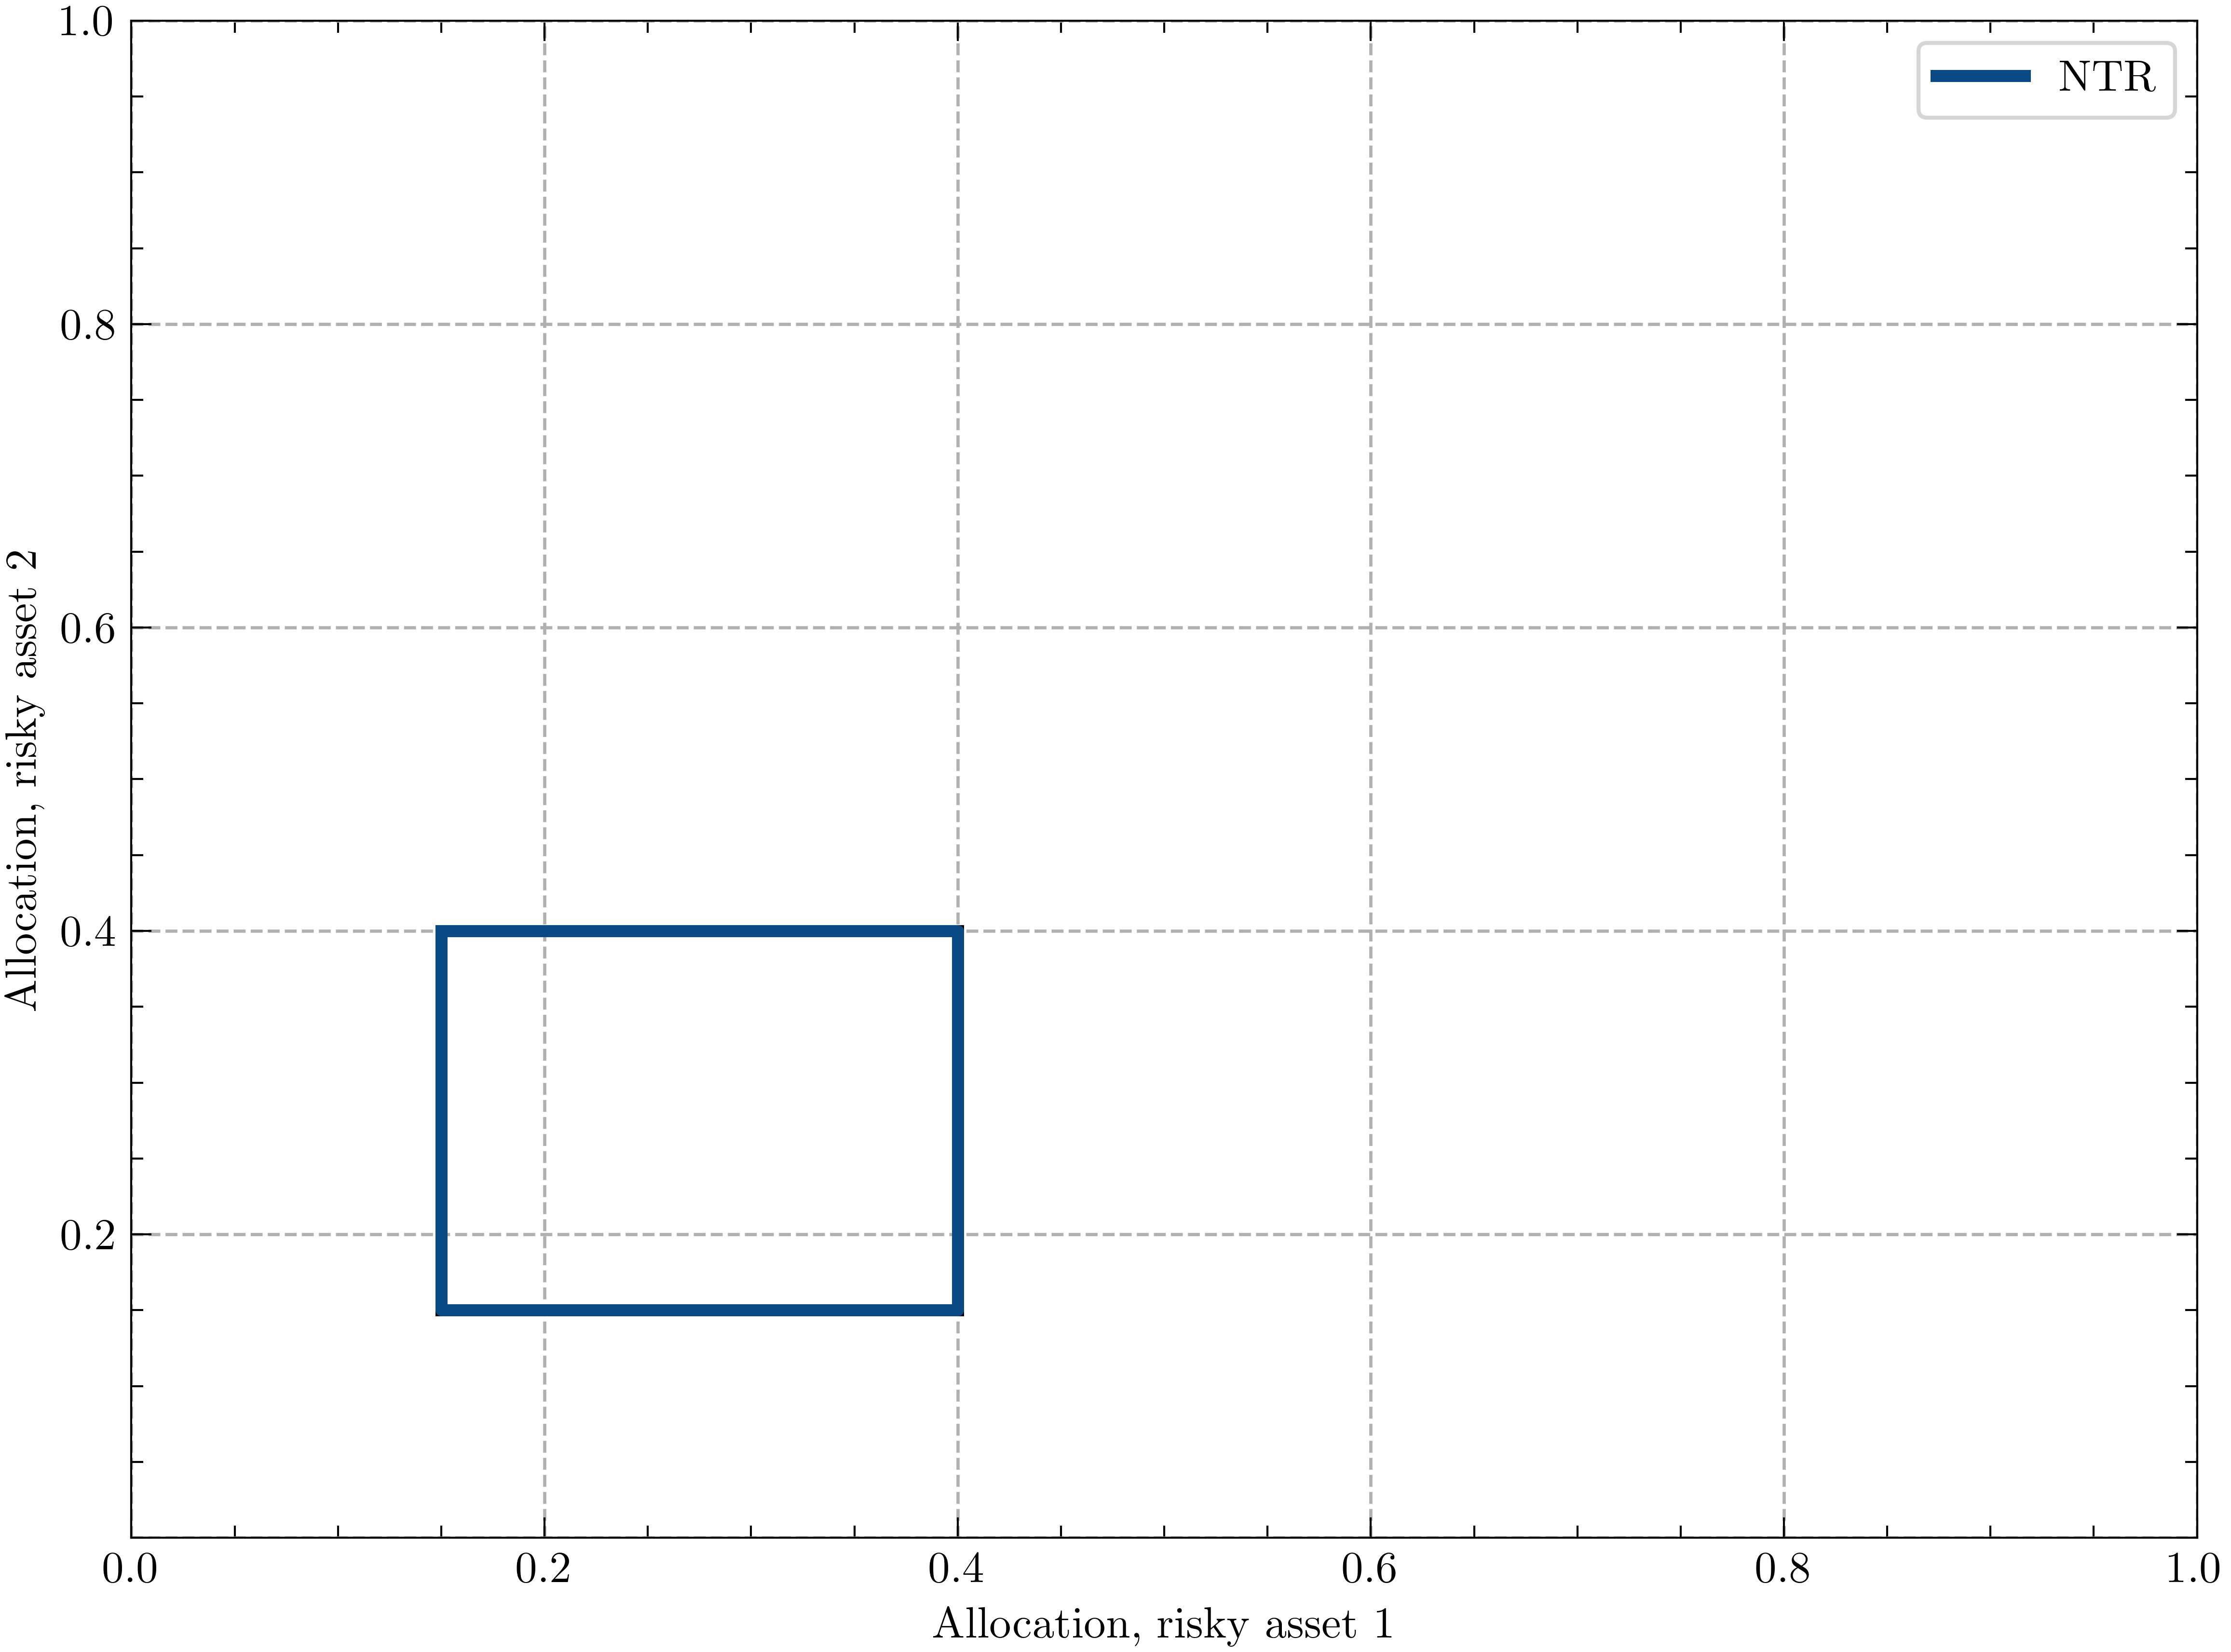
\includegraphics[scale=0.38]{Example_NTR.png}
  \end{center}
  % \floatfoot{\textbf{Note:}}
\end{figure}
The square shape of the \ac{NTR} occurs with proportional transaction costs
and independent (i.i.d) risky assets. However the NTR is not always a perfect square, for more on this see \autocite{Dybvig2020}.


\subsection{Base problem: Portfolio choice with proportional costs and consumption}\label{Subsection: Base_Problem}
Considering the class of problems constructed in the prior section,
we can now quickly introduce the basic problem formulation.
We consider an investor with CRRA utility function. She can invest in one risk free asset and $k$ risky assets.
Trading is subject to proportional transaction costs hence we have the following cost function (in cumulative terms):
\begin{equation} \label{eq: base_model_transaction-cost}
  \psi (\boldsymbol{\delta}^{+}_{i,t}, \boldsymbol{\delta}^{-}_{i,t} ) = \tau (\boldsymbol{\delta}^{+}_{i,t} + \boldsymbol{\delta}^{-}_{i,t}) 
\end{equation}
We do not assume that returns are dependent on stochastic parameters, but instead are drawn from a distribution with known parameters.
Hence we assume \( \theta_{t} = \theta \) for all $t$. That is that we assume a constant return on the risk free asset, hence $R_{f}(\theta_t) = R_{f}$,
and the risky assets follow a multivariate log-normal distribution, with some mean and covariance matrix.
We can now formulate the entire problem giventhe class structure from section \ref{Subsection: Dynamic-portfolio-choice}.
The terminal value function is given by equation \eqref{eq: class_terminal_value}. 
The system is subject to the constraints of equations \eqref{eq: No_Short_risky}, \eqref{eq: No_Short_bonds} and \eqref{eq: No_Geared_Risky},
as well as a simple constrain on consumption, $c_t \geq 0$.
We assume that the position in bond holdings is the residual wealth, and they therefore follow the process
in \eqref{eq: class_bond_holdings}. The Bellman equation is therefore:
\[  
  v_{t} (\mathbf{x}_{t}, \theta_t) = \max_{c_t , \boldsymbol{\delta}^{+}_{t}, \boldsymbol{\delta}^{-}_{t}  },  \{ u(c_t) 
  \Delta t + \beta \mathbb{E}_{t} \left[ 
    \pi_{t+\Delta t}^{1-\gamma}
    v_{t+\Delta t} (\mathbf{x}_{t+\Delta t }) 
    \right] \} , \quad t < T 
\]
With same terminal condition as before, where investments are sold and wealth is consumed.
\[
  v_T (\mathbf{x}_T) = u  (1 - \psi( \mathbf{0},\mathbf{x}_T))
\]

\subsection{Portfolio choice with fixed costs}
I now consider the model, where the investor faces fixed costs when rebalancing the portfolio, instead of proportional costs.
Fixed costs are common in practice, and can be seen as a fixed fee for trading, regardless of the traded amount.
I consider a slight modification to the classical purely fixed costs, and instead consider fixed costs as a percentage of the wealth.
I do this to be able to use the same model structure as in section \ref{Subsection: Base_Problem}, where variables are in fractions of wealth,
in order to drop wealth as a state variable.\\
This is seen previously in \autocite{morton1995optimal}, who note that such a fixed cost can be seen as a portfolio management fee.
In practice, when setting the level of the fixed cost, i make an implicit assumption on the wealth of the investor,
if i want to draw comparisons to common trading fees on the market, as the fixed cost in this scenario is purely fixed.
The cost function is then given by:
\begin{equation}
  \label{eq:Fixed_Cost_Function}
  \psi (\boldsymbol{\delta}^{+}_{t}, \boldsymbol{\delta}^{-}_{t} ) = \mathbf{1} \left(  \sum^{k}_{i=1} \delta^{+}_{i,t} + \delta^{-}_{i,t}  > 0 \right) \cdot \operatorname{fc}
\end{equation}
Where $\operatorname{fc}$ is the fixed cost, and $\mathbf{1}(\cdot)$ is the indicator function.
The fixed cost is only incurred if the investor rebalances the portfolio, and is independent of the traded amount.
The normaized bond holdings are therefore given by:
\begin{equation}\label{eq: fx_bond_holdings}
  b_{t} = 1 - \mathbf{1}^{\top} \cdot (\mathbf{x_t} - \boldsymbol{\delta}_t -) - \psi( \boldsymbol{\delta}^{+}_{t}, \boldsymbol{\delta}^{-}_{t} ) - c_t \Delta t
\end{equation}
The model otherwise remains the same as in section \ref{Subsection: Base_Problem}, with the same constraints and dynamics, while using the new cost function.
Note that in the terminal period, when all investments are sold, the fixed cost is incurred, unless the investor holds no risky assets.
Note that for the model to be well defined, the fixed cost must be less than the wealth of the investor, as the fixed cost is a percentage of the wealth.
Furthermore, the fixed cost function is not differentiable. Furthermore \autocite{Dybvig2020} notes that the fixed cost only problem,
is not a convex optimization problem, and is therefore not as easily solved as the proportional cost problem. I will deal with these issues individually
when implementing the model.
\subsection{Portfolio choice with fixed and proportional costs}
The last model i consider is a combination of the two previous models, where the investor faces both fixed and proportional costs.
This is a more realistic model, as it combines the two most common types of transaction costs an individual common investor 
face in the real world, with a fixed brokerage fee and a percentage of the traded amount stemming from bid ask spreads, taxes or commisions \autocite{Lesmond1999}.
The cost function is then given by:
\begin{equation}
  \label{eq:Fixed_Proportional_Cost_Function}
  \psi (\boldsymbol{\delta}^{+}_{t}, \boldsymbol{\delta}^{-}_{t} ) = \mathbf{1} \left(  \sum^{k}_{i=1} \delta^{+}_{i,t} + \delta^{-}_{i,t}  > 0 \right) \cdot \operatorname{fc} + \tau (\boldsymbol{\delta}^{+}_{t} + \boldsymbol{\delta}^{-}_{t})
\end{equation}
The normalized bond holdings are therefore given by:
\begin{equation}\label{eq: fx_bond_holdings}
  b_{t} = 1 - \mathbf{1}^{\top} \cdot (\mathbf{x_t} - \boldsymbol{\delta}_t -) - \psi( \boldsymbol{\delta}^{+}_{t}, \boldsymbol{\delta}^{-}_{t} ) - c_t \Delta t
\end{equation}
The model otherwise remains the same as in section \ref{Subsection: Base_Problem}, with the same constraints and dynamics, while using the new cost function.

\ifdefined\COMPILINGMAIN
% Main file is compiling this section, skip the end
\else
\printbibliography
\end{document}
\fi
\ifdefined\COMPILINGMAIN
% Main file is compiling this section, skip the preamble
\else
% Individual file compilation
\documentclass[11pt]{article}
% Geometry and page layout
\usepackage{geometry}
\geometry{verbose,tmargin=3.375cm,bmargin=2cm,lmargin=3.375cm,rmargin=3.375cm}

% Input encoding and font settings
\usepackage[utf8]{inputenc}

% other fonts
%Slightly more bold
% \usepackage{mlmodern}
% \usepackage[T1]{fontenc}

%Moder modern look
% \usepackage{libertine}
% \usepackage{libertinust1math}
% \usepackage[T1]{fontenc}

\usepackage{amsfonts, amsmath, amsthm, bbm, setspace}
\onehalfspacing
\usepackage{algorithm2e}
\usepackage{tcolorbox} % For the grey background
% Create a tcolorbox style for the algorithm
\tcbuselibrary{listingsutf8}
\tcbset{
    algobox/.style={
        colback=gray!3, % Background color
        colframe=black,  % Border color
        sharp corners,   % Square corners
        boxrule=0.5pt,   % Border thickness
        before skip=10pt, % Vertical spacing before box
        after skip=10pt,  % Vertical spacing after box
        width=\textwidth, % Box width
    }
}

% Adjust algorithm2e settings for a similar look
\SetKwInOut{Input}{Input}
\SetKwInOut{Result}{Result}
\SetKwFor{For}{for}{:}{end}

% Adjust settings for algorithm2e
\SetAlgoCaptionSeparator{.} % Separator for caption
\SetAlgoNlRelativeSize{-2}  % Adjust line number font size
\SetAlgoInsideSkip{2pt}    % Reduce space between lines
\SetAlCapSkip{0pt}         % Remove extra space after the caption
% Ensure captions are above algorithms
\SetAlgoCaptionLayout{center} % Center caption
% Adjust the style of the algorithm to remove bottom line
\RestyleAlgo{ruled}
\SetAlCapSkip{0.5em}       % Space after caption
\SetAlgoVlined              % Ensures no horizontal lines at the end

% Theorem and math environments
\newtheorem{assumption}{Assumption}
\newtheorem{lemma}{Lemma}
\newtheorem{theorem}{Theorem}

% New math commands
\newcommand{\npsym}{\mathrel{\ooalign{\raisebox{.6ex}{$>$}\cr\raisebox{-.6ex}{$<$}}}}

% Table formatting
\usepackage{booktabs, multirow, array, tabularx}
\newcolumntype{N}{>{\centering\arraybackslash}m{.85in}}

% Caption settings
\usepackage{caption}
\captionsetup{format=plain, font=footnotesize, labelfont=bf,width=3.5in}
\setlength{\abovecaptionskip}{3pt plus 3pt minus 3pt}

% Figures and floats setup
\usepackage{graphicx, adjustbox,subcaption}
\usepackage{floatrow}
\floatsetup[figure]{capposition=top}
\floatsetup[table]{capposition=top}
\renewcommand\thefigure{\thesection.\arabic{figure}}
% Path to figures
\graphicspath{{../Figures/}}
\usepackage{tikz} % TikZ for creating figures
% URLs and references and colors
\usepackage[dvipsnames]{xcolor}
\usepackage[hyphens]{url}
\usepackage{hyperref}
\hypersetup{
    colorlinks=true,
    citecolor=[HTML]{901A1E}, %KU red
    linkcolor=[HTML]{901A1E}, %KU red    
    filecolor=blue, 
    urlcolor=[HTML]{901A1E}, %KU red
    hyperindex=true,
    hyperfigures=true,
    hyperfootnotes=true,
}

% Biblatex settings for references
\usepackage[style=authoryear, dashed=false, backend=bibtex]{biblatex}
\addbibresource{../Ref.bib}

\renewbibmacro*{volume+number+eid}{%
  \printfield{volume}%
  \setunit*{\addcomma\space}%
  \printfield{number}%
  \setunit{\addcomma\space}%
  \printfield{eid}
}
\DeclareFieldFormat[article]{volume}{\bibstring{volume}~#1}
\DeclareFieldFormat[article]{number}{\bibstring{number}~#1}
\DefineBibliographyStrings{english}{volume = {Vol.}, number = {No.}}

% Author name formatting
\DeclareNameAlias{author}{last-first}
\renewcommand*{\finalnamedelim}{\addspace and\space}
\renewcommand*{\multinamedelim}{\addcomma\space}

% Footnotes and appendix setup
\usepackage[hang,flushmargin]{footmisc}
\usepackage[toc,page]{appendix}
\renewcommand\appendixtocname{Appendices}
\renewcommand\appendixpagename{Appendices}

%# Assumptions like theorems and corrolaries
% {
%   \theoremstyle{plain}
%   \newtheorem{assumption}{Assumption}
% }
% Title setup
\usepackage{titlepic}
\usepackage{titlesec}
\titleformat{\section}{\normalfont\Large\bfseries}{\thesection}{1em}{}[{\titlerule[0.1pt]}]
% no text above figures!!!!
\usepackage{placeins}

% Abbreviations (acronym package)
\usepackage{acro}
\acsetup{list/name = Abbreviations}
\DeclareAcronym{PML}{short=PML, long= Probabilistic Machine Learning}
\DeclareAcronym{NTR}{short=NTR, long=No-Trade Region}
\DeclareAcronym{MC}{short=MC, long=Monte Carlo}
\DeclareAcronym{QMC}{short=QMC, long=Quasi-Monte Carlo}
\DeclareAcronym{RQMC}{short=RQMC, long=Randomized Quasi-Monte Carlo}
\DeclareAcronym{LDS}{short = LDS, long = Low-Discrepancy Sequences}
\DeclareAcronym{LLN}{short = LLN, long = Law of Large Numbers}
\DeclareAcronym{GPR}{short = GPR, long = Gaussian process regression}
\DeclareAcronym{GP}{short = GP, long = Gaussian process}
\DeclareAcronym{ARD}{short = ARD, long = Automatic Relevance Detection}
\DeclareAcronym{LOVE}{short = LOVE, long = LanczOS Variance Estimates}
\DeclareAcronym{SKIP}{short = SKIP, long = Structured Kernel Interpolation for Products}
\DeclareAcronym{SGD}{short = SGD, long = Stochastic Gradient Descent}
\DeclareAcronym{DP}{short = DP, long = Dynamic Programming}
\DeclareAcronym{MPT}{short=MPT, long=Modern Portfolio Theory}


% Conditional macro for compiling individual files
\ifdefined\COMPILINGMAIN
% Define settings when compiling the main document
\else
% Define minimal preamble for individual file compilation
\usepackage{geometry}
\geometry{verbose,tmargin=3.375cm,bmargin=2cm,lmargin=3.375cm,rmargin=3.375cm}
\fi

\AtBeginDocument{%
    \renewcommand{\contentsname}{Table of Contents}
    \renewcommand{\abstractname}{Abstract}
}
\setlength\parindent{11pt}
% Define the macro for compiling the main file
%\def\COMPILINGMAIN{}  % Include the main preamble
\begin{document}
\fi

\section{Dynamic Portfolio choice models} \label{Section: Portfolio-choice-models}
This section covers the different portfolio choice models.
First the basic model is presented. This is followed by the most straightforward extensions,
and finally models with novel extensions are introduced.

\subsection{The general class of dynamic portfolio choice with transaction costs and intertemporal consumption} \label{Subsection: Dynamic-portfolio-choice} 
Considering the components presented in Section \ref{Section: Economic-theory},
the class of dynamic portfolio optimization problems, given one risk free asset and $k$ risky assets, can be formulated 
by the following Bellman equation, \textcite{Bellman1958}\footnote{This is consolidated model of the base model, and with consumption model, of \textcite{CaiJuddXu2020},
however the cost function is generalized and correlation of returns is included.}:
\begin{equation} \label{eq: class_bellman_non_normalized}
  V_{t} (W_t , \mathbf{x}_{t}, \theta_t) = \max_{c_t , \boldsymbol{\delta}^{+}_{t}, \boldsymbol{\delta}^{-}_{t}  } \{ u(c_t W_t ) 
  \Delta t + \beta \mathbb{E}_{t} \left[ 
    V_{t+\Delta t} (W_{t+\Delta t } \mathbf{x}_{t+\Delta t }, \theta_{t + \Delta t }  ) 
    \right] \}, \quad t < T 
\end{equation}
Given some initial level of wealth $W_0$ and portfolio allocation $\mathbf{x}_0$. \( \theta_t \) is a vector of stochastic variables, which
the gross one period risk free return, and risky return depends on, i.e \( \mathbf{R}(\theta_t) \) and \( R_f (\theta_t) \).
These could cover the drift $\mu $, volatiliy $\sigma^{2}$, correlation of the risky assets $\Sigma$, and the risk free return $r$ or only some of these, dependent on the model.
Notice that future wealth and allocations are stochastic, as they depend on the future realization of $\theta_t$.\\
Notice that consumption and reallocation are decision variables, whereas bond holding are not (Explicitly).
This is because bond holdings can be determined as the residual wealth, after consumption and reallocation decisions are made:
\begin{equation}\label{eq: class_bond_holdings_non_normalized}
  b_{t} W_t = \left( 1 - \mathbf{1}^{\top} \cdot \mathbf{x_t}  \right) W_t - \mathbf{1}^{\top} \cdot \boldsymbol{\delta}_t W_t 
  - \psi (\boldsymbol{\delta}^{+}_{t}, \boldsymbol{\delta}^{-}_t , W_t)
  - c_t W_t
\end{equation}
Where $\psi(\cdot )$ is the transaction cost function, and $\mathbf{1}$ is a vector of ones.\\
The dynamics of the state variables follow \textcite{Schober2022} and are given by:
\begin{align}
  W_{t+\Delta t} &= b_t W_t R_f (\theta_t) +  ( [ \mathbf{x_t} + \boldsymbol{\delta}_t ] W_t )^{\top} \cdot \mathbf{R}(\theta_t) \\
  \mathbf{x}_{t+\Delta t} &=  \frac{( (\mathbf{x}_t + \boldsymbol{\delta}_t ) W_t ) \odot \mathbf{R}_t (\theta_t )}{ W_{t+\Delta t} }
\end{align}
Where $\odot$ is the elementwise product (Hadamand product). The terminal value function is
given by\footnote{Stemming from the infinite sum of discounted utility of interest payments.}:
\begin{equation} \label{eq: class_terminal_value_non_normalized}
  V_T (W_T , \mathbf{x}_T , \theta_T ) = u ( ( W_T - \psi ( \mathbf{x}_T W_T )) \cdot (1-R_f (\theta_T)) )\cdot \Delta t \cdot (1-\beta)^{-1}
\end{equation}
Which implies that the investor transfers all wealth to the bank account at the terminal period,
and consumes out of the interest
returns\footnote{This formulation stems from \textcite{CaiJuddXu2013} and assumes that the investor lives forever.
\textcite{Scheidegger2023} assumes that the investor consumes everything at the terminal period.}.
Finally we note that the optimization problem is subject to the following constraints:
\begin{align}
  \boldsymbol{\delta}_t W_t &\geq - \mathbf{x}_t W_t \\
  b_t W_t &\geq 0 \\
  \mathbf{1}^{\top} \mathbf{x}_t &\leq 1
\end{align}
The first constraint ensures that the investor does not short sell risky assets, 
The second constraint is also a no shorting constraint
and the third is a no-borrowing constraint. Hence This formulation does not consider leveraged investments.\\
Furhtermore we can note that the rebalancing decision (in each direction), is only feasible in the space:
\begin{align}
  \delta^{+}_{i,t} &\in [0 , 1-x_{i,t}]  \label{eq: delta+_space} \\
  \delta^{-}_{i,t} &\in [0 , x_{i,t}] \label{eq: delta-_space}
\end{align}
This is a direct formulation of the constraints, already captured in the equations above.\\
The problem can be simplified by normalizing wrt. wealth, and removing wealth as a state variable, since
wealth is seperable from the rest of the state space $\mathbf{x}_t , \theta_t$ as noted by \textcite{CaiJuddXu2013}.\\
This is because portfolio optimality is independent of wealth for CRRA utility function. 
The Bellman equation is then:
\begin{equation} \label{eq: class_bellman}
  v_{t} (\mathbf{x}_{t}, \theta_t) = \max_{c_t , \boldsymbol{\delta}^{+}_{t}, \boldsymbol{\delta}^{-}_{t} } \{ u(c_t) 
  \Delta t + \beta \mathbb{E}_{t} \left[ 
    \pi_{t+\Delta t}^{1-\gamma}
    v_{t+\Delta t} (\mathbf{x}_{t+\Delta t }, \theta_{t + \Delta t }  ) 
    \right] \} , \quad t < T 
\end{equation}
The normalized bond holdings are then:
\begin{equation}\label{eq: class_bond_holdings}
  b_{t} = 1 - \mathbf{1}^{\top} \cdot (\mathbf{x_t} - \boldsymbol{\delta}_t - \psi( \boldsymbol{\delta}^{+}_{t}, \boldsymbol{\delta}^{-}_{t}  )) - c_t \Delta t
\end{equation}
We see that these are still the residual of the wealth after the rebalancing and consumption decision.
Where we formulate the transaction cost function $\psi(\cdot)$ in terms of the buying and selling components,
and using changes to allocations proportional to wealth, instead of the prior formulations, where wealth was a direct input.
The dynamics are then:
\begin{align}
  \pi_{t+\Delta t} &= b_t R_f (\theta_t)  + (\mathbf{x}_t + \boldsymbol{\delta}_t)^{\top} \cdot \mathbf{R}(\theta_t) \\
  \mathbf{x}_{t+\Delta t} &=  \frac{(\mathbf{x}_t + \boldsymbol{\delta}_t) \odot \mathbf{R}_t (\theta_t )}{ \pi_{t+\Delta t} } \\
  W_{t+\Delta t} &= \pi_{t+\Delta t} W_t
\end{align}
Where we now formulate the problem with regard to the proportional wealth change $\pi_{t+\Delta t} = \frac{W_{t+\Delta t}}{W_t}$.
The terminal value function is:
\begin{equation} \label{eq: class_terminal_value}
  v_T (\mathbf{x}_T , \theta_T ) = u ( (1 - \psi(\mathbf{x}_T)) \cdot (1-R_f (\theta_T)) )\cdot \Delta t \cdot (1-\beta)^{-1} 
\end{equation}
The constrains are likewise normalized:
\begin{align}
  \boldsymbol{\delta}_t &\geq - \mathbf{x}_t \label{eq: No_Short_risky} \\
  b_t &\geq 0 \label{eq: No_Short_bonds}\\
  \mathbf{1}^{\top} \mathbf{x}_t &\leq 1 \label{eq: No_Geared_Risky}
\end{align}
This class of dynamic portfolio choice problems covers any formulation of the problem,
where the transaction cost specification is differentiable, and the utility function allows for seperability of wealth and remaining state variables.
Later formulations will be based on this class structure, covering the necessary Bellman equaiton, state dynamics, preferences and transaction costs functions as well as the constraints
and any extensions not yet presented.
\subsection{Base problem: Portfolio with proportional costs and consumption}\label{Subsection: Base_Problem}
Considering the class of problems constructed in the prior section,
we can now quickly introduce the basic problem formulation.
We consider an investor with CRRA utility function. She can invest in one risk free asset and $k$ risky assets.
Trading is subject to proportional transaction costs hence we have the following cost function (in cumulative terms):
\begin{equation} \label{eq: base_model_transaction-cost}
  \psi (\boldsymbol{\delta}^{+}_{i,t}, \boldsymbol{\delta}^{-}_{i,t} ) = \tau (\boldsymbol{\delta}^{+}_{i,t} + \boldsymbol{\delta}^{-}_{i,t}) 
\end{equation}
We do not assume that returns are dependent on stochastic parameters, but instead are drawn from a distribution with known parameters.
Hence we assume \( \theta_{t} = \theta \) for all $t$. That is that we assume a constant return on the risk free asset, hence $R_{f}(\theta_t) = R_{f}$,
and the risky assets follow a multivariate log-normal distribution, with some mean and covariance matrix.
We can now formulate the entire problem giventhe class structure from section \ref{Subsection: Dynamic-portfolio-choice}.
The terminal value function is given by equation \eqref{eq: class_terminal_value}. 
The system is subject to the constraints of equations \eqref{eq: No_Short_risky}, \eqref{eq: No_Short_bonds} and \eqref{eq: No_Geared_Risky},
as well as a simple constrain on consumption, $c_t \geq 0$.
We assume that the position in bond holdings is the residual wealth, and they therefore follow the process
in \eqref{eq: class_bond_holdings}. The Bellman equation is therefore:
\[  
  v_{t} (\mathbf{x}_{t}, \theta_t) = \max_{c_t , \boldsymbol{\delta}^{+}_{t}, \boldsymbol{\delta}^{-}_{t}  },  \{ u(c_t) 
  \Delta t + \beta \mathbb{E}_{t} \left[ 
    \pi_{t+\Delta t}^{1-\gamma}
    v_{t+\Delta t} (\mathbf{x}_{t+\Delta t }) 
    \right] \} , \quad t < T 
\]
With same terminal condition as before, where wealth is transfered to the bond account at the terminal period, 
and consumption is financed by the interest returns.
\[
  v_T (\mathbf{x}_T) = u ( (1 - \psi( \mathbf{0},\mathbf{x}_T)) \cdot (1-R_f) )\cdot \Delta t \cdot (1-\beta)^{-1} 
\]

\subsection{Portfolio with fixed and proportional costs}
\subsection{Portfolio with asset specific costs}

\ifdefined\COMPILINGMAIN
% Main file is compiling this section, skip the end
\else
\printbibliography
\end{document}
\fi
\ifdefined\COMPILINGMAIN
% Main file is compiling this section, skip the preamble
\else
% Individual file compilation
\documentclass[11pt]{article}
% Geometry and page layout
\usepackage{geometry}
\geometry{verbose,tmargin=3.375cm,bmargin=2cm,lmargin=3.375cm,rmargin=3.375cm}

% Input encoding and font settings
\usepackage[utf8]{inputenc}

% other fonts
%Slightly more bold
% \usepackage{mlmodern}
% \usepackage[T1]{fontenc}

%Moder modern look
% \usepackage{libertine}
% \usepackage{libertinust1math}
% \usepackage[T1]{fontenc}

\usepackage{amsfonts, amsmath, amsthm, bbm, setspace}
\onehalfspacing
\usepackage{algorithm2e}
\usepackage{tcolorbox} % For the grey background
% Create a tcolorbox style for the algorithm
\tcbuselibrary{listingsutf8}
\tcbset{
    algobox/.style={
        colback=gray!3, % Background color
        colframe=black,  % Border color
        sharp corners,   % Square corners
        boxrule=0.5pt,   % Border thickness
        before skip=10pt, % Vertical spacing before box
        after skip=10pt,  % Vertical spacing after box
        width=\textwidth, % Box width
    }
}

% Adjust algorithm2e settings for a similar look
\SetKwInOut{Input}{Input}
\SetKwInOut{Result}{Result}
\SetKwFor{For}{for}{:}{end}

% Adjust settings for algorithm2e
\SetAlgoCaptionSeparator{.} % Separator for caption
\SetAlgoNlRelativeSize{-2}  % Adjust line number font size
\SetAlgoInsideSkip{2pt}    % Reduce space between lines
\SetAlCapSkip{0pt}         % Remove extra space after the caption
% Ensure captions are above algorithms
\SetAlgoCaptionLayout{center} % Center caption
% Adjust the style of the algorithm to remove bottom line
\RestyleAlgo{ruled}
\SetAlCapSkip{0.5em}       % Space after caption
\SetAlgoVlined              % Ensures no horizontal lines at the end

% Theorem and math environments
\newtheorem{assumption}{Assumption}
\newtheorem{lemma}{Lemma}
\newtheorem{theorem}{Theorem}

% New math commands
\newcommand{\npsym}{\mathrel{\ooalign{\raisebox{.6ex}{$>$}\cr\raisebox{-.6ex}{$<$}}}}

% Table formatting
\usepackage{booktabs, multirow, array, tabularx}
\newcolumntype{N}{>{\centering\arraybackslash}m{.85in}}

% Caption settings
\usepackage{caption}
\captionsetup{format=plain, font=footnotesize, labelfont=bf,width=3.5in}
\setlength{\abovecaptionskip}{3pt plus 3pt minus 3pt}

% Figures and floats setup
\usepackage{graphicx, adjustbox,subcaption}
\usepackage{floatrow}
\floatsetup[figure]{capposition=top}
\floatsetup[table]{capposition=top}
\renewcommand\thefigure{\thesection.\arabic{figure}}
% Path to figures
\graphicspath{{../Figures/}}
\usepackage{tikz} % TikZ for creating figures
% URLs and references and colors
\usepackage[dvipsnames]{xcolor}
\usepackage[hyphens]{url}
\usepackage{hyperref}
\hypersetup{
    colorlinks=true,
    citecolor=[HTML]{901A1E}, %KU red
    linkcolor=[HTML]{901A1E}, %KU red    
    filecolor=blue, 
    urlcolor=[HTML]{901A1E}, %KU red
    hyperindex=true,
    hyperfigures=true,
    hyperfootnotes=true,
}

% Biblatex settings for references
\usepackage[style=authoryear, dashed=false, backend=bibtex]{biblatex}
\addbibresource{../Ref.bib}

\renewbibmacro*{volume+number+eid}{%
  \printfield{volume}%
  \setunit*{\addcomma\space}%
  \printfield{number}%
  \setunit{\addcomma\space}%
  \printfield{eid}
}
\DeclareFieldFormat[article]{volume}{\bibstring{volume}~#1}
\DeclareFieldFormat[article]{number}{\bibstring{number}~#1}
\DefineBibliographyStrings{english}{volume = {Vol.}, number = {No.}}

% Author name formatting
\DeclareNameAlias{author}{last-first}
\renewcommand*{\finalnamedelim}{\addspace and\space}
\renewcommand*{\multinamedelim}{\addcomma\space}

% Footnotes and appendix setup
\usepackage[hang,flushmargin]{footmisc}
\usepackage[toc,page]{appendix}
\renewcommand\appendixtocname{Appendices}
\renewcommand\appendixpagename{Appendices}

%# Assumptions like theorems and corrolaries
% {
%   \theoremstyle{plain}
%   \newtheorem{assumption}{Assumption}
% }
% Title setup
\usepackage{titlepic}
\usepackage{titlesec}
\titleformat{\section}{\normalfont\Large\bfseries}{\thesection}{1em}{}[{\titlerule[0.1pt]}]
% no text above figures!!!!
\usepackage{placeins}

% Abbreviations (acronym package)
\usepackage{acro}
\acsetup{list/name = Abbreviations}
\DeclareAcronym{PML}{short=PML, long= Probabilistic Machine Learning}
\DeclareAcronym{NTR}{short=NTR, long=No-Trade Region}
\DeclareAcronym{MC}{short=MC, long=Monte Carlo}
\DeclareAcronym{QMC}{short=QMC, long=Quasi-Monte Carlo}
\DeclareAcronym{RQMC}{short=RQMC, long=Randomized Quasi-Monte Carlo}
\DeclareAcronym{LDS}{short = LDS, long = Low-Discrepancy Sequences}
\DeclareAcronym{LLN}{short = LLN, long = Law of Large Numbers}
\DeclareAcronym{GPR}{short = GPR, long = Gaussian process regression}
\DeclareAcronym{GP}{short = GP, long = Gaussian process}
\DeclareAcronym{ARD}{short = ARD, long = Automatic Relevance Detection}
\DeclareAcronym{LOVE}{short = LOVE, long = LanczOS Variance Estimates}
\DeclareAcronym{SKIP}{short = SKIP, long = Structured Kernel Interpolation for Products}
\DeclareAcronym{SGD}{short = SGD, long = Stochastic Gradient Descent}
\DeclareAcronym{DP}{short = DP, long = Dynamic Programming}
\DeclareAcronym{MPT}{short=MPT, long=Modern Portfolio Theory}


% Conditional macro for compiling individual files
\ifdefined\COMPILINGMAIN
% Define settings when compiling the main document
\else
% Define minimal preamble for individual file compilation
\usepackage{geometry}
\geometry{verbose,tmargin=3.375cm,bmargin=2cm,lmargin=3.375cm,rmargin=3.375cm}
\fi

\AtBeginDocument{%
    \renewcommand{\contentsname}{Table of Contents}
    \renewcommand{\abstractname}{Abstract}
}
\setlength\parindent{11pt}
% Define the macro for compiling the main file
%\def\COMPILINGMAIN{}  % Include the main preamble
\begin{document}
\fi

\section{Numerical implementation details} \label{Section: Implmentation-details}
This section covers detail regarding the solution algorithm and numerical implementation.
Each method is presented in a separate subsection, and the final solution algorithm is presented in the last subsection,
which combines each of the methods. These span points sampling, numerical integration techniques, function approximation methods
and solution techniques specific to this class of problemns.
\subsection{Numerical integration} \label{Subsection: NumericalIntegration}
Consider the basic problem with proportional transaction costs, basic risky assets and a risk-free asset and no stochastic parameters.
We need to evaluate the expectation of the value function:
$\mathbb{E} \left[ v_{t+\Delta t} (\mathbf{x}_{t+\Delta t }  ) \right]$.
In order to compue this expectation, we need to evaluate the integral:
\begin{equation}
  \mathbb{E}_{t} \left[ \pi_{t+1}^{1-\gamma} v_{t+1} (x_{t+1}) \right] = \int \pi_{t+1}^{1-\gamma} v_{t+1} (x_{t+1}) f(R_{t+1}), d R_{t+1}
\end{equation}
where $f(R_{t+1})$ is the probability density function of the risky asset returns. If we look at the case of stochastic parameters, 
would need to evaluate the conditional expectation with regard to these aswell, given some distributional assumption on the parameters.
The integral can be computed using Monte-carlo methods
or by using quadrature rules.
\subsubsection{Gauss-Hermite quadrature} \label{Subsection: Gauss-Hermite}
Gaussian quadrature is a numerical integration method based on approximation and interpolation theory.
Gaussian quadrature can be used to approximate integrals using the following form, \textcite{Judd1998Book}:
\begin{equation}
  \int_{a}^{b} f(x) w(x) dx \approx \sum_{i=1}^{n} \omega_{i} f(x_{i}),
\end{equation}
Where $\omega_i$ are quadrature weights, $x_i$ are quadrature nodes and $w(x)$ is a weighting function.
This approximation is exact when $f(x)$ is a polynomial of degree $2n-1$ or less.
Then we can approximate the integral using $n$ points $x_i$ and $n$ weights $\omega_i$.
There are many different Gaussian quadrature schemes, with differering intervals $[a,b]$ and weighting functions $w(x)$.
We consider the use of a Gauss-Hermite quadrature rule, for a comprehensive review on Gaussian quadrature rules, see \textcite{Judd1998Book}.
Gauss-Hermite quadrature is used to approximate integrals of the form:
\begin{equation}
  \int_{-\infty}^{\infty} f(x) e^{-x^{2}} dx \approx \sum_{i=1}^{n} \omega_{i} f(x_{i}) + \frac{n! \sqrt{\pi}}{2^{n}} 
  \cdot \frac{f^{(2n) }(\zeta )}{(2n)!},
\end{equation}
Where $\zeta \in (-\infty , \infty)$.
If a random variable $X$ is normally distributed, i.e  $X \sim \mathcal{N}(\mu , \sigma^{2})$,
then we can compute the expectation, $\mathbb{E}[f(X)]$, which is given by:
\begin{equation}
  \mathbb{E} [f(X)] =  \frac{1}{\sqrt{2\pi \sigma^{2}} } \int_{-\infty}^{\infty} f(x)  e^{-\frac{(x-\mu)^{2}}{2\sigma^{2}}} dx 
\end{equation}
Using a change of variables $y = \frac{x-\mu}{\sqrt{2}\sigma}$, then we can rewrite the expectation on the form of the Gauss-Hermite quadrature rule:
\begin{align}
  \mathbb{E} [f(X)] &=  \frac{1}{\sqrt{2\pi \sigma^{2}} } \int_{-\infty}^{\infty} f( \sqrt{2} \sigma y + \mu)  e^{-y^{2}} \sqrt{2} \sigma dy \\
  &= \frac{1}{\sqrt{\pi}} \int_{-\infty}^{\infty} e^{-y^{2}} f( \sqrt{2} \sigma y + \mu) dy \\
  &\approx \frac{1}{\sqrt{\pi}} \sum_{i=1}^{n} \omega_{i} f( \sqrt{2} \sigma x_{i} + \mu)
\end{align}
Where $\omega_i$ are the quadrature weights, $x_i$ are the quadrature nodes over the interval $(-\infty , \infty)$.\\
When $X$ is log-normal, i.e $\log X \sim \mathcal{N}(\mu , \sigma^{2})$, then we can use a variable change once again:
$X = e^{Y}$ and $Y \sim \mathcal{N}(\mu , \sigma^{2})$. Then we can rewrite the expectation as:
\begin{equation}
  \mathbb{E} [ f(X) ] = \mathbb{E} [ f(e^{Y}) ] \approx \pi^{-\frac{1}{2}} \sum{n}_{i=1} \omega_i f \left( e^{ \sqrt{2} \sigma x_{i} + \mu } \right)
\end{equation}

If we want to extend this framework to multiple dimensions we can use product rules as noted by \textcite{CaiJuddXu2013}.
Consider $Y$ which is multivariate normal, i.e $Y \sim \mathcal{N}(\boldsymbol{\mu} , \Sigma)$,
where $\mu$ is the drift vector and $\Sigma$ is the covariance matrix.
Let $L$ be a lower-triangular matrix such that $LL^{\top} = \Sigma$ (Cholesky factorisation).
Then we have that:
\begin{align}
  \mathbb{E}\{f(Y)\} & = \left( (2\pi)^d \det(\Sigma) \right)^{-\frac{1}{2}} \int_{\mathbb{R}^d} f(y) \, e^{-\frac{1}{2}(y - \mu)^{\top} \Sigma^{-1} (y - \mu)} \, dy \\
  & = \left( (2\pi)^d \det(L)^2 \right)^{-\frac{1}{2}} \int_{\mathbb{R}^d} f\left(\sqrt{2} L y + \mu\right) \, e^{-\frac{1}{2} y^{\top} y} \, dy \\
  & \approx \pi^{-\frac{d}{2}} \sum_{i_1=1}^n \cdots \sum_{i_d=1}^n \omega_{i_1} \cdots \omega_{i_d} \, f
  \bigg(\sqrt{2} L_{1,1} y_{i_1} + \mu_1, \;
  \notag \\
  & \quad \sqrt{2} (L_{2,1} y_{i_1} + L_{2,2} y_{i_2}) + \mu_2, \;
  \ldots, \;
  \sqrt{2} \big(\sum_{j=1}^d L_{d,j} y_{i_j}\big) + \mu_d
  \bigg) 
  \end{align}
Where $d$ refers to the number of dimensions, $n$ is the number of quadrature points, $\omega_i$ are the quadrature weights and $y_i$ are the quadrature nodes.
$L_{i,j}$ is the $i$th row and $j$th column of the Cholesky factorisation matrix $L$. $\det$ is the matrix determinant.
We note that the use of product rules suffers from the curse of dimensionality, 
as the complexity scales exponentionally with the number of dimensions. This is because the quadrature points with the product rule,
normally use a tensor product grid, which is constructed using the Cartesian product of the quadrature points in each dimension.
We can use sparse grid methods to partially tackle this. One common method  is the Smolyak method, \textcite{smolyak1963}.
Smolyaks sparse grid method approximates multidimensional integrals, over dimesion $d$
while limiting the amount of points used. The method is composed of the following:
\begin{enumerate}
  \item \textbf{Univariate Quadrature Rules}: Each dimension of the integration domain is assigned a univariate quadrature rule, which provides both nodes (quadrature points) and weights for numerical integration in that dimension. The accuracy of each rule is determined by its \textit{level}, denoted by \( i_d \) for each dimension \( d \). The level determines the number of quadrature points in that dimension, which improves the accuracy of the quadrature rule. 
  
  \item \textbf{Approximation Level (\( \mu \))}: The accuracy of the Smolyak sparse grid is controlled by the \textit{approximation level} \( \mu \). This parameter sets a limit on the sum of levels across all dimensions, controlling the total number of grid points. Higher values of \( \mu \) result in more accurate approximations but increase computational complexity.

  \item \textbf{Multi-Index and Combination of Levels}: In a \( d \)-dimensional integral, the Smolyak method uses a \textit{multi-index} \( i = (i_1, i_2, \dots, i_d) \) to represent the level of the quadrature rule in each dimension. The multi-index specifies a unique combination of quadrature levels for each dimension, where \( i_d \) denotes the level for dimension \( d \). To construct a sparse grid, Smolyak’s method restricts the sum of these levels using the following condition:
  \[
  d \leq i_1 + i_2 + \dots + i_d \leq d +  \mu
  \]
  This constraint on the sum of levels, reduces the number of tensor products. We denote the sum of multi indicies: $\lvert i \rvert = i_1 + i_2 + \dots i_d$.

  \item \textbf{Tensor Product of Univariate Rules}: The Smolyak grid is formed by taking the \textit{tensor product} of univariate quadrature rules that satisfy the multi-index constraint. Each univariate quadrature rule, represented by \( Q_{i_d} \) at level \( i_d \) in dimension \( d \), is combined across dimensions according to the set of multi-indices \( i \). This combination is given by:
  \[
  A(\mu, d) = \sum_{d \leq |i| \leq d + \mu} (-1)^{\mu + d - |i|} \binom{d - 1}{\mu + d - 1 - |i|} \bigotimes_{d=1}^d Q_{i_d}
  \]
  where:
  \begin{itemize}
      \item \( Q_{i_d} \) is the univariate quadrature rule at level \( i_d \) in dimension \( d \),
      \item \( \bigotimes \) denotes the tensor product, and
      \item \( \binom{d - 1}{\mu + d - 1 - |i|} \) is a combinatorial coefficient that assigns weights to each tensor product, for accurate integration up to the specified approximation level \( \mu \).
  \end{itemize} 
\end{enumerate}
By resticting the multi indicies \( i \) with the approximation level \( \mu \), the Smolyak method reduces 
the number of points needed for numerical integration in higher dimensions.
Tensor grid methods grows exponentially with the number of dimensions \( d \), the Smolyak grid grows polynomially, \textcite{judd2014smolyak},
hence it directly combats the curse of dimensionality. For more on this see \textcite{smolyak1963}, \textcite{judd2014smolyak} and
\textcite{horneff2016efficient}. 

\subsubsection{Monte Carlo integration (MC)} \label{Subsection: MC}
Monte Carlo integration is a numerical integration method based on \textit{sampling}, as opposed to
quadrature rules which are based on interpolation. \\
The convergence of Monte Carlo integration is generally slower
than some quadrature methods; however, its convergence rate is independent of
the dimensionality of the integral, making it well-suited for high-dimensional problems.
Monte Carlo integration breaks the curse of dimensionality.
\ac{MC} integration is based on random sampling\footnote{Strictly speaking the samples are not random, but pseudo-random, meaning that deterministic samples are used, which appear random. For more in this see \textcite{Judd1998Book} or  \textcite{Glasserman2004MC}}
over the domain of the integral, and then computing the sample average of the function to be integrated.
Assume we wish to approximate the $d$-dimensional integral:
\begin{equation} \label{eq: MC-integral}
  I = \int_{\Omega} f(\mathbf{x}) g(\mathbf{x}) d\mathbf{x} = \mathbb{E}[f(\mathbf{x})],
\end{equation}
where \( g(\mathbf{x}) \) is the probability density function of the random variable \( \mathbf{x} \) over its support \( \Omega \), we approximate \( I \) as:
\begin{equation} \label{eq: MC-integralapproximation}
  Q_N = \frac{1}{N} \sum_{i=1}^{N} f(\mathbf{X}_i),
\end{equation}
where \( \mathbf{X}_i \) are independent samples drawn from \( g(\mathbf{x}) \).
The procedure is then:
\begin{enumerate}
  \item Sample \( N \) points \( \mathbf{x}_1, \ldots, \mathbf{x}_N \) from \( g(\mathbf{x}) \).
  \item Approximate the expectation \( \mathbb{E}[f(\mathbf{x})] \) by the sample average:
\end{enumerate}
\[
I \approx Q_{N} = \frac{1}{N} \sum_{i=1}^{N} f(\mathbf{x}_{i}).
\]
The Law of Large Numbers ensures that the sample average converges to the mean as \( N \to \infty \):
\[
\lim_{{N \to \infty}} Q_{N} = \mathbb{E}[f(\mathbf{x})] = I.
\]
And by the Central Limit Theorem, we have:
\[
\sqrt{N} \left( Q_N - I \right) \xrightarrow{d} N\left(0, \sigma^2 \right),
\]
where \( \sigma^2 = \operatorname{Var}[f(\mathbf{x})] \) does not depend on \( N \) or \( d \). 
The standard error of \( Q_N \) is:
\[
\sigma_{Q_N} = \frac{\sigma}{\sqrt{N}}.
\]
The convergence rate of \( 1/\sqrt{N} \) is independent of the dimension. 
\subsubsection{Quasi-Monte Carlo integration (QMC)} \label{Subsubsection: QMC}
Quasi-Monte Carlo integration substitutes the 'random' samples in Monte Carlo integration 
with specific deterministic sequences such as equidistributred sequences, \ac{LDS} or Lattice point rules etc.
We will focus on the use of low discrepancy sequences. For a comprehesive review of sequences and rules see \textcite{Judd1998Book}.\\
\ac{LDS} are deterministic sequences which cover the domain of the integral more evenly than random samples. 
Discrepancy is in this case a measure of deviation from perfect uniformity over the domain of the integral.
Thus to go from MC in \eqref{eq: MC-integralapproximation} to QMC, we replace the random samples $\mathbf{X}_i$ with \ac{LDS} samples.
We note that the sampling of the QMC is now dependent on the dimensionality of the integral, as opposed to MC,
as the LDS samples have to be drawn with respect to the dimensionality of the integral.

We consider two different types of \ac{LDS} sequences, the Halton sequence and the Sobol sequence.
Both sequences are popular \ac{LDS} sequences,
which are used in \ac{QMC} applications, \autocite{Glasserman2004MC}.

The convergence rate of \ac{QMC} is:
\begin{equation} \label{eq: QMC-convergence}
  \frac{\left( \log N \right)^{d}}{N}
\end{equation}
Hence QMC is generally faster than MC, e.g $\frac{\left( \log N \right)^{d}}{N} < \frac{1}{\sqrt{N}}$ for large $N$ and small $d$.
We note that as dimensionality $d$ increases, the quality of the Halton sequence decreases, as the dimensions become more correlated, \textcite{Glasserman2004MC}.
Specifically the Halton seuqnce will produce diagonal points when projected onto a 2D plane.
This is displayed in figure \ref{fig: Sampling_comparison_MC_D1D2}. 
We therefore prefer the Sobol sequence when the dimensionality is sufficiently high,
and as not to complicate matters, also use the Sobol sequence in lower dimensions, when \ac{QMC} schemes are used.
Figures below shows Random samples, Halton samples and Sobol samples in 2d.
Second figure shows the same in 18 dimensions. Halton shows that dimension 17 and 18 are correlated.
\begin{figure}[h!]
  \begin{center}
  \caption{Comparison of sample generation for Monte Carlo and Quasi-Monte Carlo} 
  \label{fig: Sampling_comparison_MC_D1D2}
  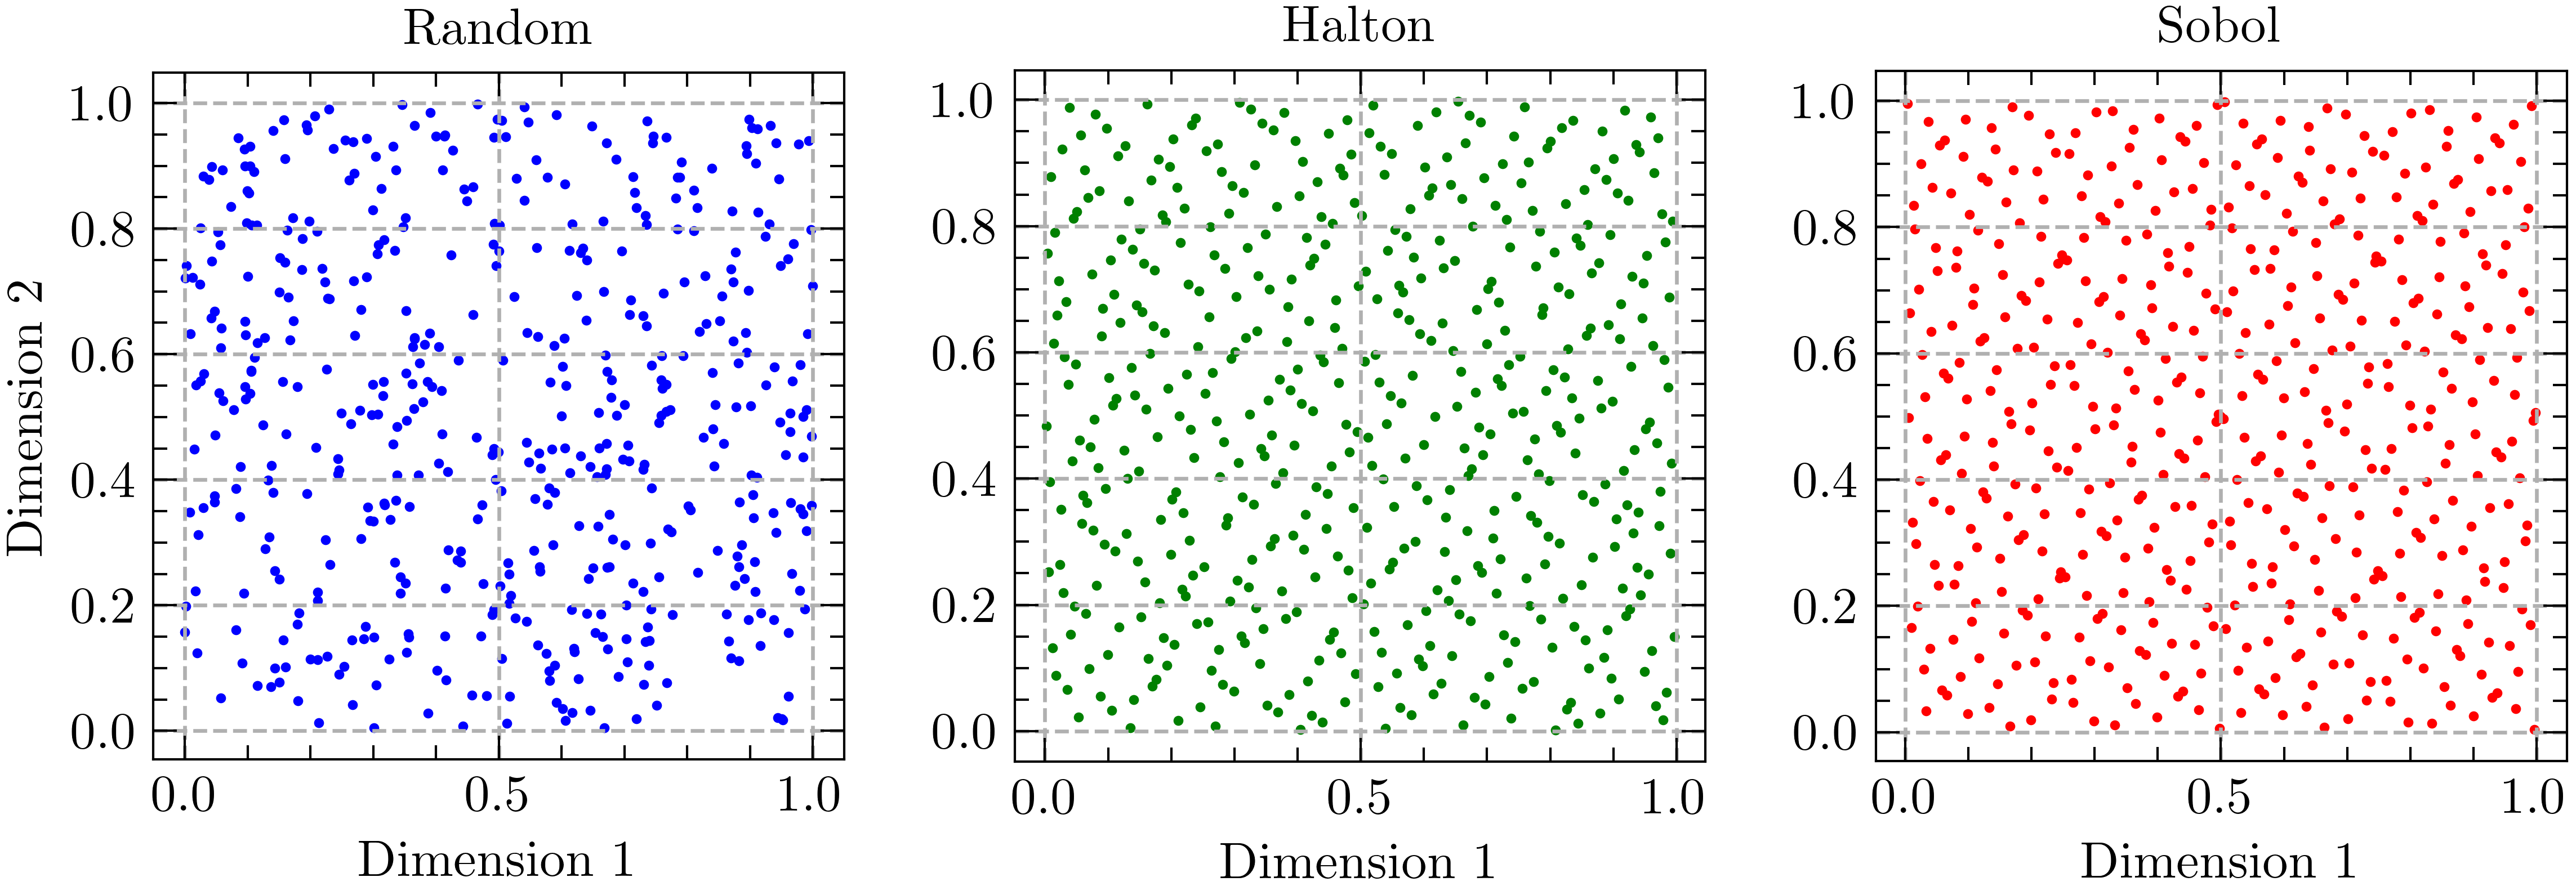
\includegraphics[width=\textwidth]{sampling_comparison_d1_d2.png}
  \end{center}
  \floatfoot{\textbf{Note:} 
  Each sequence was generated using $N = 500$ samples and $d = 2$ dimensions.}
\end{figure}

\begin{figure}[h!]
  \begin{center}
  \caption{Comparison of sample generation for Monte Carlo and Quasi-Monte Carlo with increased dimensionality} 
  \label{fig: Sampling_comparison_MC_D17D18}
  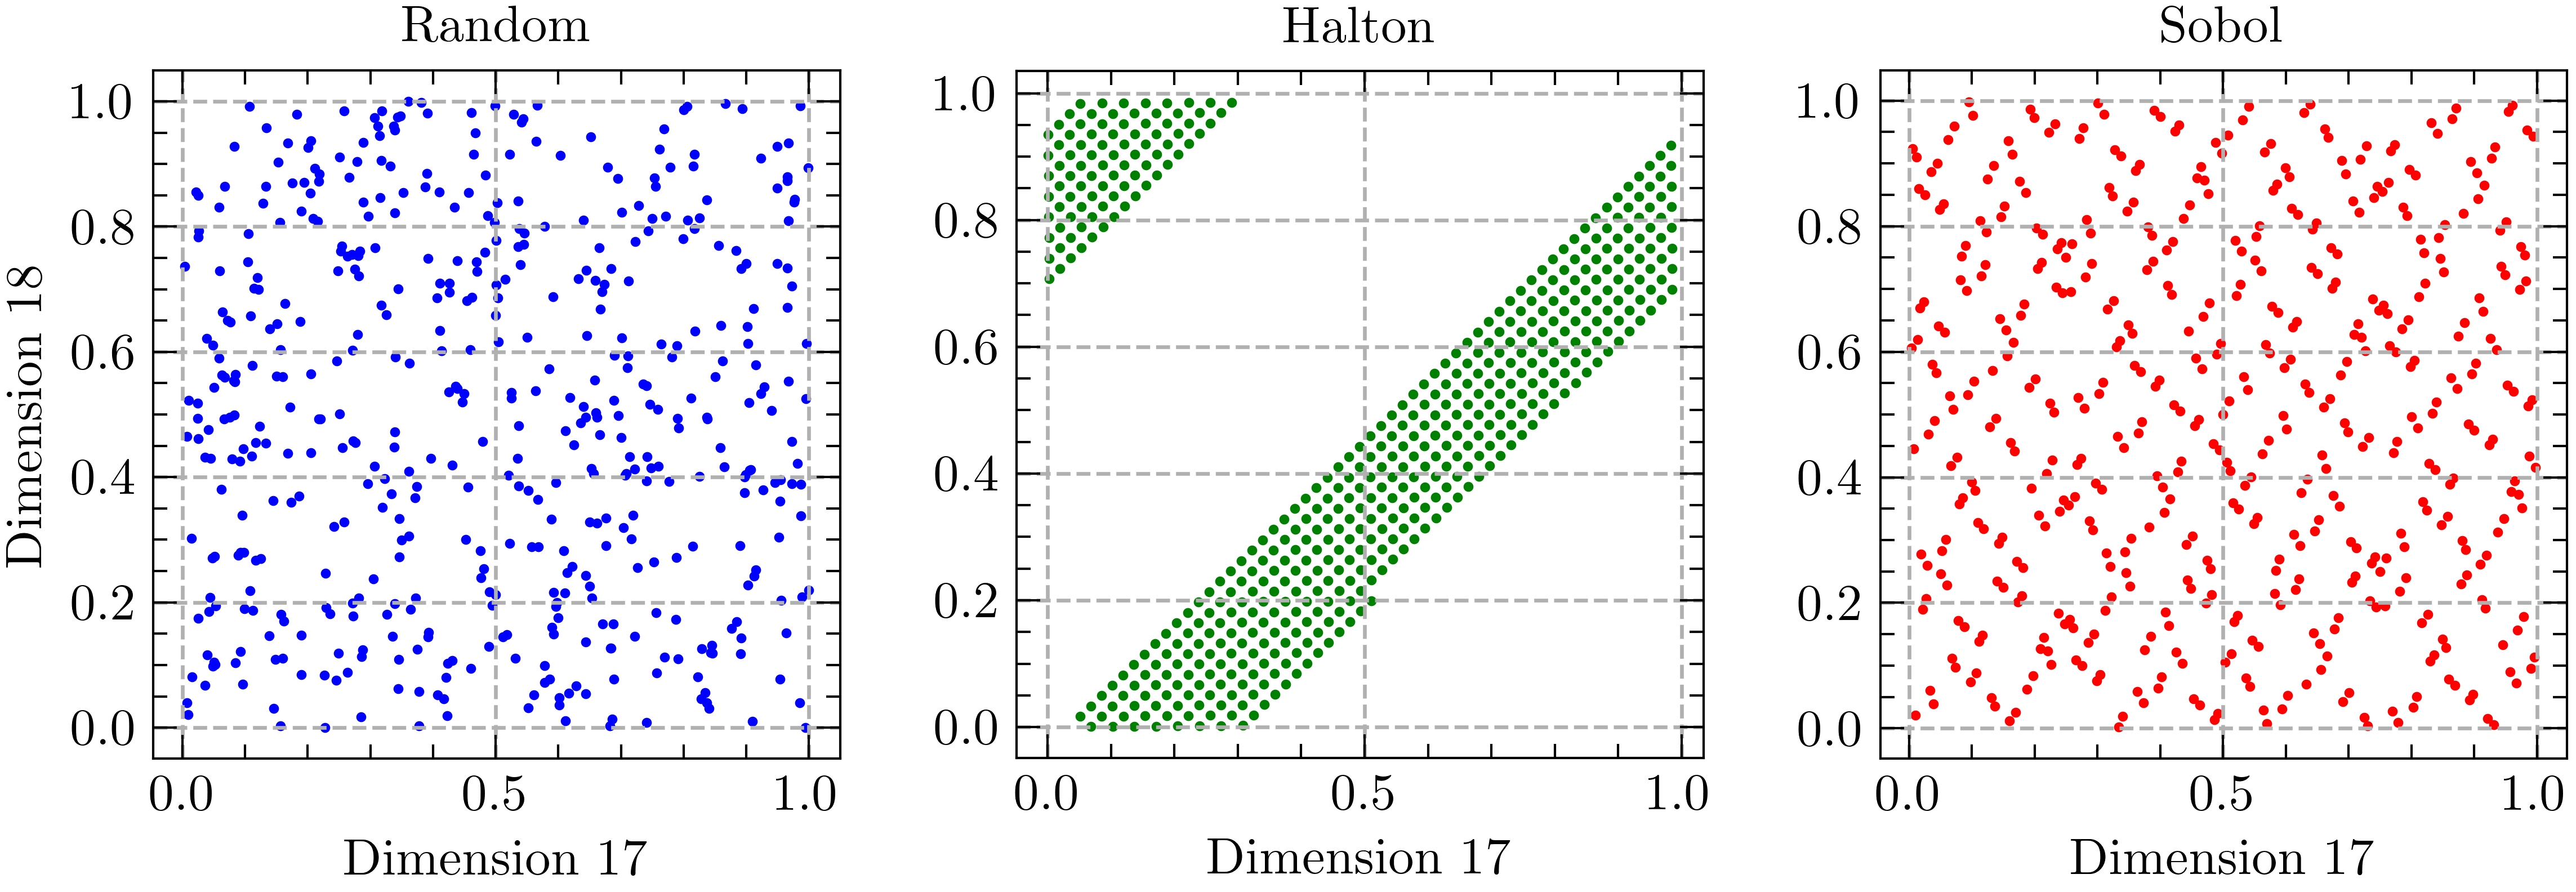
\includegraphics[width=\textwidth]{sampling_comparison_d17_d18.png}
  \end{center}
  \floatfoot{\textbf{Note:} 
  Each sequence was generated using $N = 500$ samples and $d = 18$ dimensions.}
\end{figure}
QMC is generally found to be more efficient than MC, as noted by \textcite{Glasserman2004MC}, \textcite{Judd1998Book},
and notably Glasserman find that dimensionality has to be quite large before the Monte Carlo method is favorable to the quasi Monte Carlo method.
Furthermore Glasserman find that while we generally might assume that $N$ must by increase a lot when $d$ is increased, this is not
always the case in classic financial applications, as the integrals employed in these examples can often
be approximated by integrals of much lower dimension. QMC therefore performs better than to be expected.

However we note that \ac{QMC} lacks a straightforward variance estimator,
a feature recovered through \textit{randomized QMC}, which will be discussed in the next section.

\subsubsection{Randomized Quasi-Monte carlo integration (RQMC)} \label{Subsection: RQMC}
Randomized quasi-Monte Carlo integration (RQMC) is a combination of \ac{QMC} and \ac{MC} integration.
We consider the the QMC integral, i.e the equaiton of \eqref{eq: MC-integralapproximation}, using an \ac{LDS} sequence.
The point of \ac{RQMC} is then to introduce randomness to the sequence: $P_{n} = \{ x_1 , \ldots , x_n \}$.
We will cover the most simple case, \textit{Random shift} and \textit{Scrambling} methods, however for a comprehensive review of randomization methods see \textcite{Glasserman2004MC}.
The most simple method of randomizing $P_n$ is to add a \textit{random shift} to each point in the sequence, using
random numbers drawn from a uniform distribution of the same dimensionality as the sequence, wrapped to the interval of $P_n$.
Hence if $x_{i} \in [0,1)^{d}$ then we add a random shift $u_{i} \operatorname{mod} 1$, where
$\operatorname{mod} 1$ keeps the shift within the interval $[0,1)$. 
A major disadvantage of the random shift is that is changes the discrepancy properties of the sequence,
and hence the quality of the sequence is lost.\\
Scrambled nets is a method of randomization which can be applied to \ac{LDS} sequences specifically.
Scrambling works by applying a sequence of random permutations to the 
digits in the base-b representation of each coordinate in the \ac{LDS}.
Each digit is permuted based on the values of the digits that came before it. 
This structure retains the low-discrepancy properties 
while introducing a controlled level of randomness, 
which enables the calculation of variance for RQMC estimates.
In multi-dimensional settings, this scrambling is applied independently to each coordinate of the sequence, allowing us to estimate variance across the entire space.
Scrambling the Sobol sequence has been found to be particularily effective in financial applications,
as noted by \textcite{Scramble2023}. QMC is generally more efficient than MC, and RQMC increases the rate of converence of QMC
and allows for the estimation of variance.  
\subsection{Value function approximation}
This section covers the necessary function approximation methods used in the solution algorithm.
We will cover the use of \ac{GPR} and Baysian optimization, in order to maximize the value function of the dynamic portfolio allocation problem. 


\subsubsection{Gaussian process regressions (GPR)} \label{Subsubsection: GPR}
A \ac{GP} is a probabilistic model that defines a distribution over functions used to make predictions based on available data. 
It is specified by two functions: the mean function and the covariance function, also called the kernel. 
The mean function, \( m(\mathbf{x}) \), represents the expected value of the function at a given input \( \mathbf{x} \), 
and the covariance function, \( k(\mathbf{x}, \mathbf{x}') \), 
captures the covariance between function values at different input points \( \mathbf{x} \) and \( \mathbf{x}' \).
In a \ac{GP}, any finite set of input points \( \mathbf{X} = (\mathbf{x}_1, \dots, \mathbf{x}_N) \) within the domain \( \mathbb{R}^d \) 
results in the function values \( \mathbf{f} = (f(\mathbf{x}_1), \dots, f(\mathbf{x}_N)) \) having a joint multivariate Gaussian distribution.
This property enables a GP to provide a prior distribution over functions based on the defined mean and covariance.

We use \ac{GPR} to estimate the value function in the dynamic portfolio allocation problem,
when we are not at the terminal period, i.e., \( t < T \), following \textcite{Scheidegger2023}.
The \ac{GP} is formulated by the previously mentioned mean and covariance functions:
\begin{equation} \label{eq: GP-definition}
  f(\mathbf{x}) \sim \mathcal{GP}(m(\mathbf{x}), k(\mathbf{x}, \mathbf{x}')),
\end{equation}
The covariance kernel function \( k(\mathbf{x}, \mathbf{x}') \) can be any Mercer kernel, i.e., positive definite \autocite{MurphyBook2023}.
Common kernel choices include the Radial Basis Function (RBF) kernel, the Matern kernel, and the Exponential kernel.
We employ a Matern kernel, which, depending on the parameter \( \nu \), 
can be a generalization of the RBF kernel or the Exponential kernel. This choice follows \textcite{Scheidegger2023}.
The Matern kernel is given by:
\begin{equation} \label{eq: Matern-kernel}
  k_{\text{Matern}}(\mathbf{x} , \mathbf{x}') = \frac{2^{1-\nu}}{\Gamma(\nu)}  \left( \frac{\sqrt{2 \nu} \| \mathbf{x} - \mathbf{x}' \|_{2}}{\ell} \right) K_{\nu} \left( \frac{\sqrt{2 \nu} \| \mathbf{x} - \mathbf{x}' \|_{2}}{\ell} \right),
\end{equation}
where \( \| \cdot \|_{2} \) is the Euclidean norm, \( \Gamma \) is the gamma function, and \( K_{\nu} \) is the modified Bessel function.
The length scale \( \ell \) and smoothness parameter \( \nu \) are both positive. As \( \nu \to \infty \), the Matern kernel converges to the RBF kernel \autocite{Gonzalvez2019}.
Functions from this class are \( k \)-times differentiable when \( \nu > k \).
When \( \nu = 1/2 \), the Matern kernel corresponds to the Ornstein-Uhlenbeck process \autocite{MurphyBook2023},
which is commonly used in financial applications, such as models of interest rates \autocite{Glasserman2004MC}. 

Consider a training dataset \( \{ \mathbf{X}, \mathbf{y} \} \)
with \( N \) states \( \mathbf{x}_{i} \) and observed values \( \mathbf{y} \). 
We assume that the observations \( \mathbf{y} \) are generated by an unknown function \( f \), such that
\[
y_i = f(\mathbf{x}_i) + \varepsilon_{i}, \quad \varepsilon_{i} \sim \mathcal{N}(0, \sigma^{2}_{\varepsilon}),
\]
where \( \sigma^{2}_{\varepsilon} \) represents the observational noise\footnote{The noise assumption implies that the GP model does not interpolate the data but rather fits a smooth function. 
This results in computational costs of \( O(N) \) for the mean prediction and \( O(N^2) \) for the variance prediction. For more details, see \autocite{MurphyBook2023}.}.
The goal is to train a \ac{GP} on this dataset and then use it to predict the value function at a new state \( \mathbf{x}_{*} \),
yielding a new predicted output \( f_{*} \).

The training observations \( \mathbf{y} \) and the predicted noise-free function \( f_{*} \) 
have a joint Gaussian distribution:
\begin{equation}\label{eq: GP-distribution}
  \begin{bmatrix}
    \mathbf{y} \\
    \mathbf{f}_{*}
  \end{bmatrix}
  \sim 
  \mathcal{N} \left( \mathbf{0},
                \begin{bmatrix}
                  k(\mathbf{X}, \mathbf{X}) + \sigma^{2}_{\varepsilon} \mathbf{I} & k(\mathbf{X}, \mathbf{x}_{*}) \\
                  k(\mathbf{x}_{*}, \mathbf{X}) & k(\mathbf{x}_{*}, \mathbf{x}_{*})
                \end{bmatrix}
              \right)
\end{equation}
Here i have assumed a zero mean function\footnote{Zero mean ... XXXX}, and the kernel function is the Matern kernel.
The posterior distribution of the predicted value function \( f_{*} \) given the training data is then a multivariate normal \autocite{MurphyBook2023},
with mean:
\begin{equation} \label{eq: GP-pred-mean}
  \tilde{\mu}(\mathbf{x}) = k(\mathbf{x}_{*}, \mathbf{X}) [k(\mathbf{X}, \mathbf{X}) + \sigma^{2}_{\varepsilon} \mathbf{I}]^{-1} \mathbf{y},
\end{equation}
And covariance:
\begin{equation} \label{eq: GP-pred-covariance}
 \tilde{k} (\mathbf{x}_* , \mathbf{x}_{*}^{'}) = 
 k (\mathbf{x}_* , \mathbf{x}_{*}^{'}) - 
 k (\mathbf{x}_* , \mathbf{X}) 
  [k (\mathbf{X} , \mathbf{X}) + \sigma^{2}_{\varepsilon} \mathbf{I}]^{-1}
  k (\mathbf{X} , \mathbf{x}_{*}^{'})
\end{equation}
Therefore in order to predict the value function at a new state $\mathbf{x}_{*}$, we need to compute the mean and covariance.
This step is computationally burdensome as we have to compute the four covariance matrices in the joint distribution \eqref{eq: GP-distribution}.
Afterwards we can compute predictions using the mean function \eqref{eq: GP-pred-mean} and the covariance function \eqref{eq: GP-pred-covariance}
can be used to compute error bands on our predictions. 

As noted, training and predicting with a \ac{GP} is computationally expensive. I will therefore introduce
the methods employed to reduce the computational burden of the \ac{GP}.

We use automatic relevance detection (ARD) which is a modification to the Matern kernel to use
a length scale for each dimension, $\ell_{i}$. Dimensions with low impact has a high length scale, and are effectively ignored.
Note that this is not the same as Lasso, as these coefficients are not set to $0$.
We use \ac{SKIP} to reduce the computational burden of computen the matrices in the joint distribution \eqref{eq: GP-distribution}.

\textbf{Use LancZos Variance Estimate (Love) and SKIP to reduce computational burden.}\\
Here is the documentation in my package 
\url{https://docs.gpytorch.ai/en/stable/examples/02_Scalable_Exact_GPs/index.html} 

And here is a paper on the subject \url{https://arxiv.org/pdf/1803.06058}.
\subsection{Approximating the No trade region} \label{Subsection: Approximating_NTR}
Since i now have introduced methods to approximate the next-period value function $v_{t+1}$, and methods for evaluating the expectation $\mathbb{E}[\cdot]$
over known distributions, we can now approximate the \ac{NTR} using a \ac{DP} scheme. In order to do this some assummptions regarding the unknown NTR are formed,
these are drawn directly from \autocite{Scheidegger2023}
\begin{assumption}\label{assumption: NTR-convex}
  The NTR is a $D$-dimensional convex polytope.
\end{assumption}
A polytope is a generalization of a polyhedron (polytope in 2D), which is a geometric object with flat sides and straight edges.
  The convex polytope is a polytope which bounds a convex set, and can therefore be defined by a convex hull. Hence, any linear combination of points in the \ac{NTR} or on the boundary of the \ac{NTR} is also in the \ac{NTR}.
  In other words, the \ac{NTR} is a closed convex set. \textbf{Wikipedia reference her?}.
\begin{assumption}\label{assumption: NTR-vertices}
  The NTR has $2^{D}$ vertices.
\end{assumption}
This assumption is regarding the shape of the \ac{NTR}. Note that if the actual \ac{NTR} has less than $2^{D}$ vertices, the approximation will be close to the actual shape, as the approximated vertices will be on top of each other.
However if the \ac{NTR} as more then $2^{D}$ vertices, then the approximation will be a simplification of the actual shape. 
The existing litterature finds that the \ac{NTR} is a $D$-dimensional parallelogram, this is formally shown with uncorrelated assets by \autocite{liu2002}, and with correlated assets the same is found by \autocite{CaiJuddXu2013,Dybvig2020}.
Hence i believe this sampling scheme to be sufficient, for the case of proportional transaction costs.

\autocite{Dybvig2020} find that the \ac{NTR} is a circle or ellipse when there are only fixed costs, and when there are asset specifc costs the \ac{NTR} is a hexagon in the 2D case, as one vertice is added per asset.
This would suggest other sampling schemes for these cases. For the circular case i would need to sample evenly around the circle (sphere / hypersphere), this problem is well known in mathematics and computer graphics and many methods for this exists,
among others lattice point methods. For more on this see for example \autocite{UNSWsphere} or \autocite{delbono2024}.
For the hexagon case, i could add more midpoints between the vertices of the existing sampling scheme. 

With these two assumptions in place, a strategy for approximating the \ac{NTR} can be formed with few initial points.
Given assumption \ref{assumption: NTR-vertices} we can approximate the \ac{NTR} by using $2^{D}$ points, which are the vertices of the \ac{NTR},
and by assumption \ref{assumption: NTR-convex} we can approximate the \ac{NTR} by using the convex hull of these points, i.e connecting the vertices by straight lines to form the outer hull.

I can leverage the following intution from \autocite{Scheidegger2023}, and from \ref{fig: NTR_Example}: For any point outside the \ac{NTR},
the optimal policy is to trade towards the boundary of the \ac{NTR}. Since each point on the boundary of the NTR is optimal, the optimal trading route minimizes the
distance, and hence the optimal trading route is a straight line to the boundary of the \ac{NTR}. If the points ahre chosen correctly, the optimal trading route will be to a vertex of the \ac{NTR}.
This is seen in the figure below:\\
\begin{figure}[!ht]
  \centering
  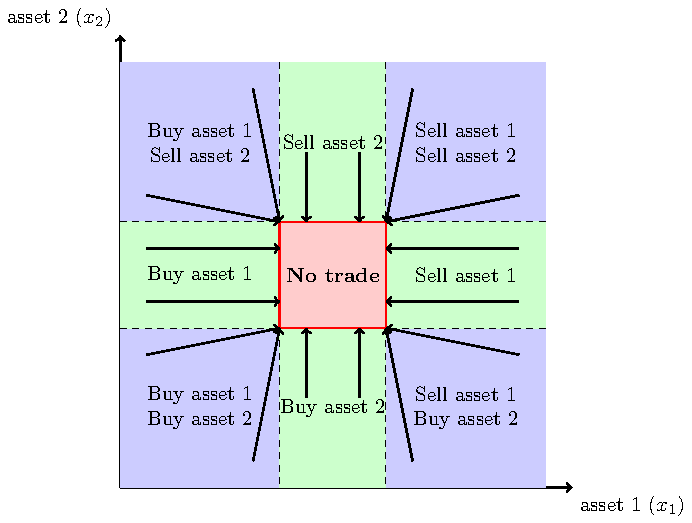
\includegraphics[width=0.5\textwidth]{../Sections/tikzfigure.pdf} % Path to your PDF file
  \caption{Illustration of the no-trade region (NTR) and the optimal policies outside this.}
  \label{fig:no_trade_region_schematic}
  % add float foot
  \floatfoot{This is a schematic NTR. Blue regions are regions where optimal policy $\boldsymbol{\delta}$ is to adjust both asset allocations.
  Green regions are regions where the optimal policy is to hold in one asset and adjust the other. This figure is a recreation of Figure 1. in \textcite{Scheidegger2023}.}
\end{figure}
If one considers the example in figure \ref{fig:no_trade_region_schematic}, i can effectively approximate the \ac{NTR},
by sampling a point in each of the blue regions, and then solving the optimization problem to find the vertices.
When the \ac{NTR} is unknown, sampling from the blue regions seem difficult at a first glance.
However, i can sample the vertices of each simplex that covers the feasible space, and the midpoints between these.
This sampling scheme leads to the following points in the $2$-dimensional case:
\[
  \begin{bmatrix}
    0 & 0 \\
    1 & 0 \\
    0 & 1 \\
    0.5 & 0.5 
  \end{bmatrix}
\]
Extensions of this sampling scheme to higher dimensions is trivial.
This should effectively cover the feasible space, and allow for approximating the \ac{NTR}. Note that this sampling scheme only covers \ac{NTR}
with no borrowing, and no short-selling as noted in \autocite{Scheidegger2023}. If borrowing and short-selling were introduced, we would have to set some bounds on the borrowing and short-selling,
and then sample from these bounds. Effectively creating a square (cube / hypercube), around the feasible space, and then sample the vertices of this space.

Having approximated the \ac{NTR}, we can now use this in the solution algorithm. There are two main ways which the \ac{NTR} approximation can be leveraged in order to
lessen the computational burden of the solution algorithm. these will be covered below.
\subsubsection{Strategic point sampling} \label{subsubsection: Sample}
After having approximated the \ac{NTR} i need to efficiently approximate the value function in the time step related to the \ac{NTR}. 
This is done by sampling points over the entire feasible space, and then solving for the optimal trade route for each point.
In order to ensure that the approximation of the value function is of high quality, and that this value function can effectively be used for any point in the state space,
we need to ensure that the points are sampled in a strategic manner. This means i need points of a few different types:
I need points inside the NTR, and around the \ac{NTR} in any direction, and various distances to the \ac{NTR}.
This leads to three types of points i need to sample: \textit{Points inside the \ac{NTR}}, \textit{points near the kinks of the \ac{NTR}} and \textit{points in the general state space, outside the \ac{NTR}}.
An easily implemntable solution is to use a naive grid sampling method, such as uniform draws over the feasible state space, or to use a grid-method which evenly covers the feasible state space. 
However, a simple naive grid method for sampling points over the state-space has a few drawbacks which i need to tackle.

First of all, a naive grid method, such as uniform draws, will not cover the \ac{NTR} efficiently, especially for small \ac{NTR}s.
I would need a large amount of grid points to be sure that there are multiple points inside the NTR.
A pure random grid would likewise need a large amount of points, in order to cover the \ac{NTR} efficiently, especially in each direction around the NTR.
Both of these methods, and a schematic \ac{NTR} are shown in appendix \ref{section: Appendix-sample}.\\
I therefore instead follow the method of \autocite{Scheidegger2023}, and sample points in a strategic manner.
This scheme consists of the three point types mentioned earlier, with a sampling method for each of these points.
Having approximated the \ac{NTR}, i can effectivly sample point in this manner:
\begin{enumerate}
  \item Sample points outside the \ac{NTR} in the general state space using a uniform grid. I then remove all points inside the \ac{NTR}, and sample random grid points until i have enough points.
  \item Sample points inside the \ac{NTR}. For this i consider random draws, as the placement inside the NTR is not of high importance. I just need enough to approximate the value function.
  \item Sample points around the \ac{NTR} kinks. For this i consider each \ac{NTR} vertice. I then interpolate between adjacent vertices slightly, and extend these outward with random noise draws. 
\end{enumerate}
The resulting points are plotted in figure \ref{fig: Designed_sampling_strategy}, and a zoom in on the \ac{NTR} kinks are shown in figure \ref{fig: Designed_sampling_strategy-zoom}.
\autocite{Scheidegger2023} find that especially increased sampling around the kinks, leads to a better approximation of the value function,
and $N>100$ points leads to sufficient approximations, as most of the approximation error is due to the kinks of the \ac{NTR}.
This choice of sampling scheme furthermore reduces the strain by curse of dimensionality, as grid sampling schemes would increase the number of points exponentially with the number of dimensions.
Note that while this scheme still increases the number of points needed with the dimensionality, the oversampling of grid points especially reduce the number of points needed in higher dimensions.

\begin{figure}[!ht]
  \centering
    \begin{subfigure}[t]{0.48\textwidth}
        \centering
        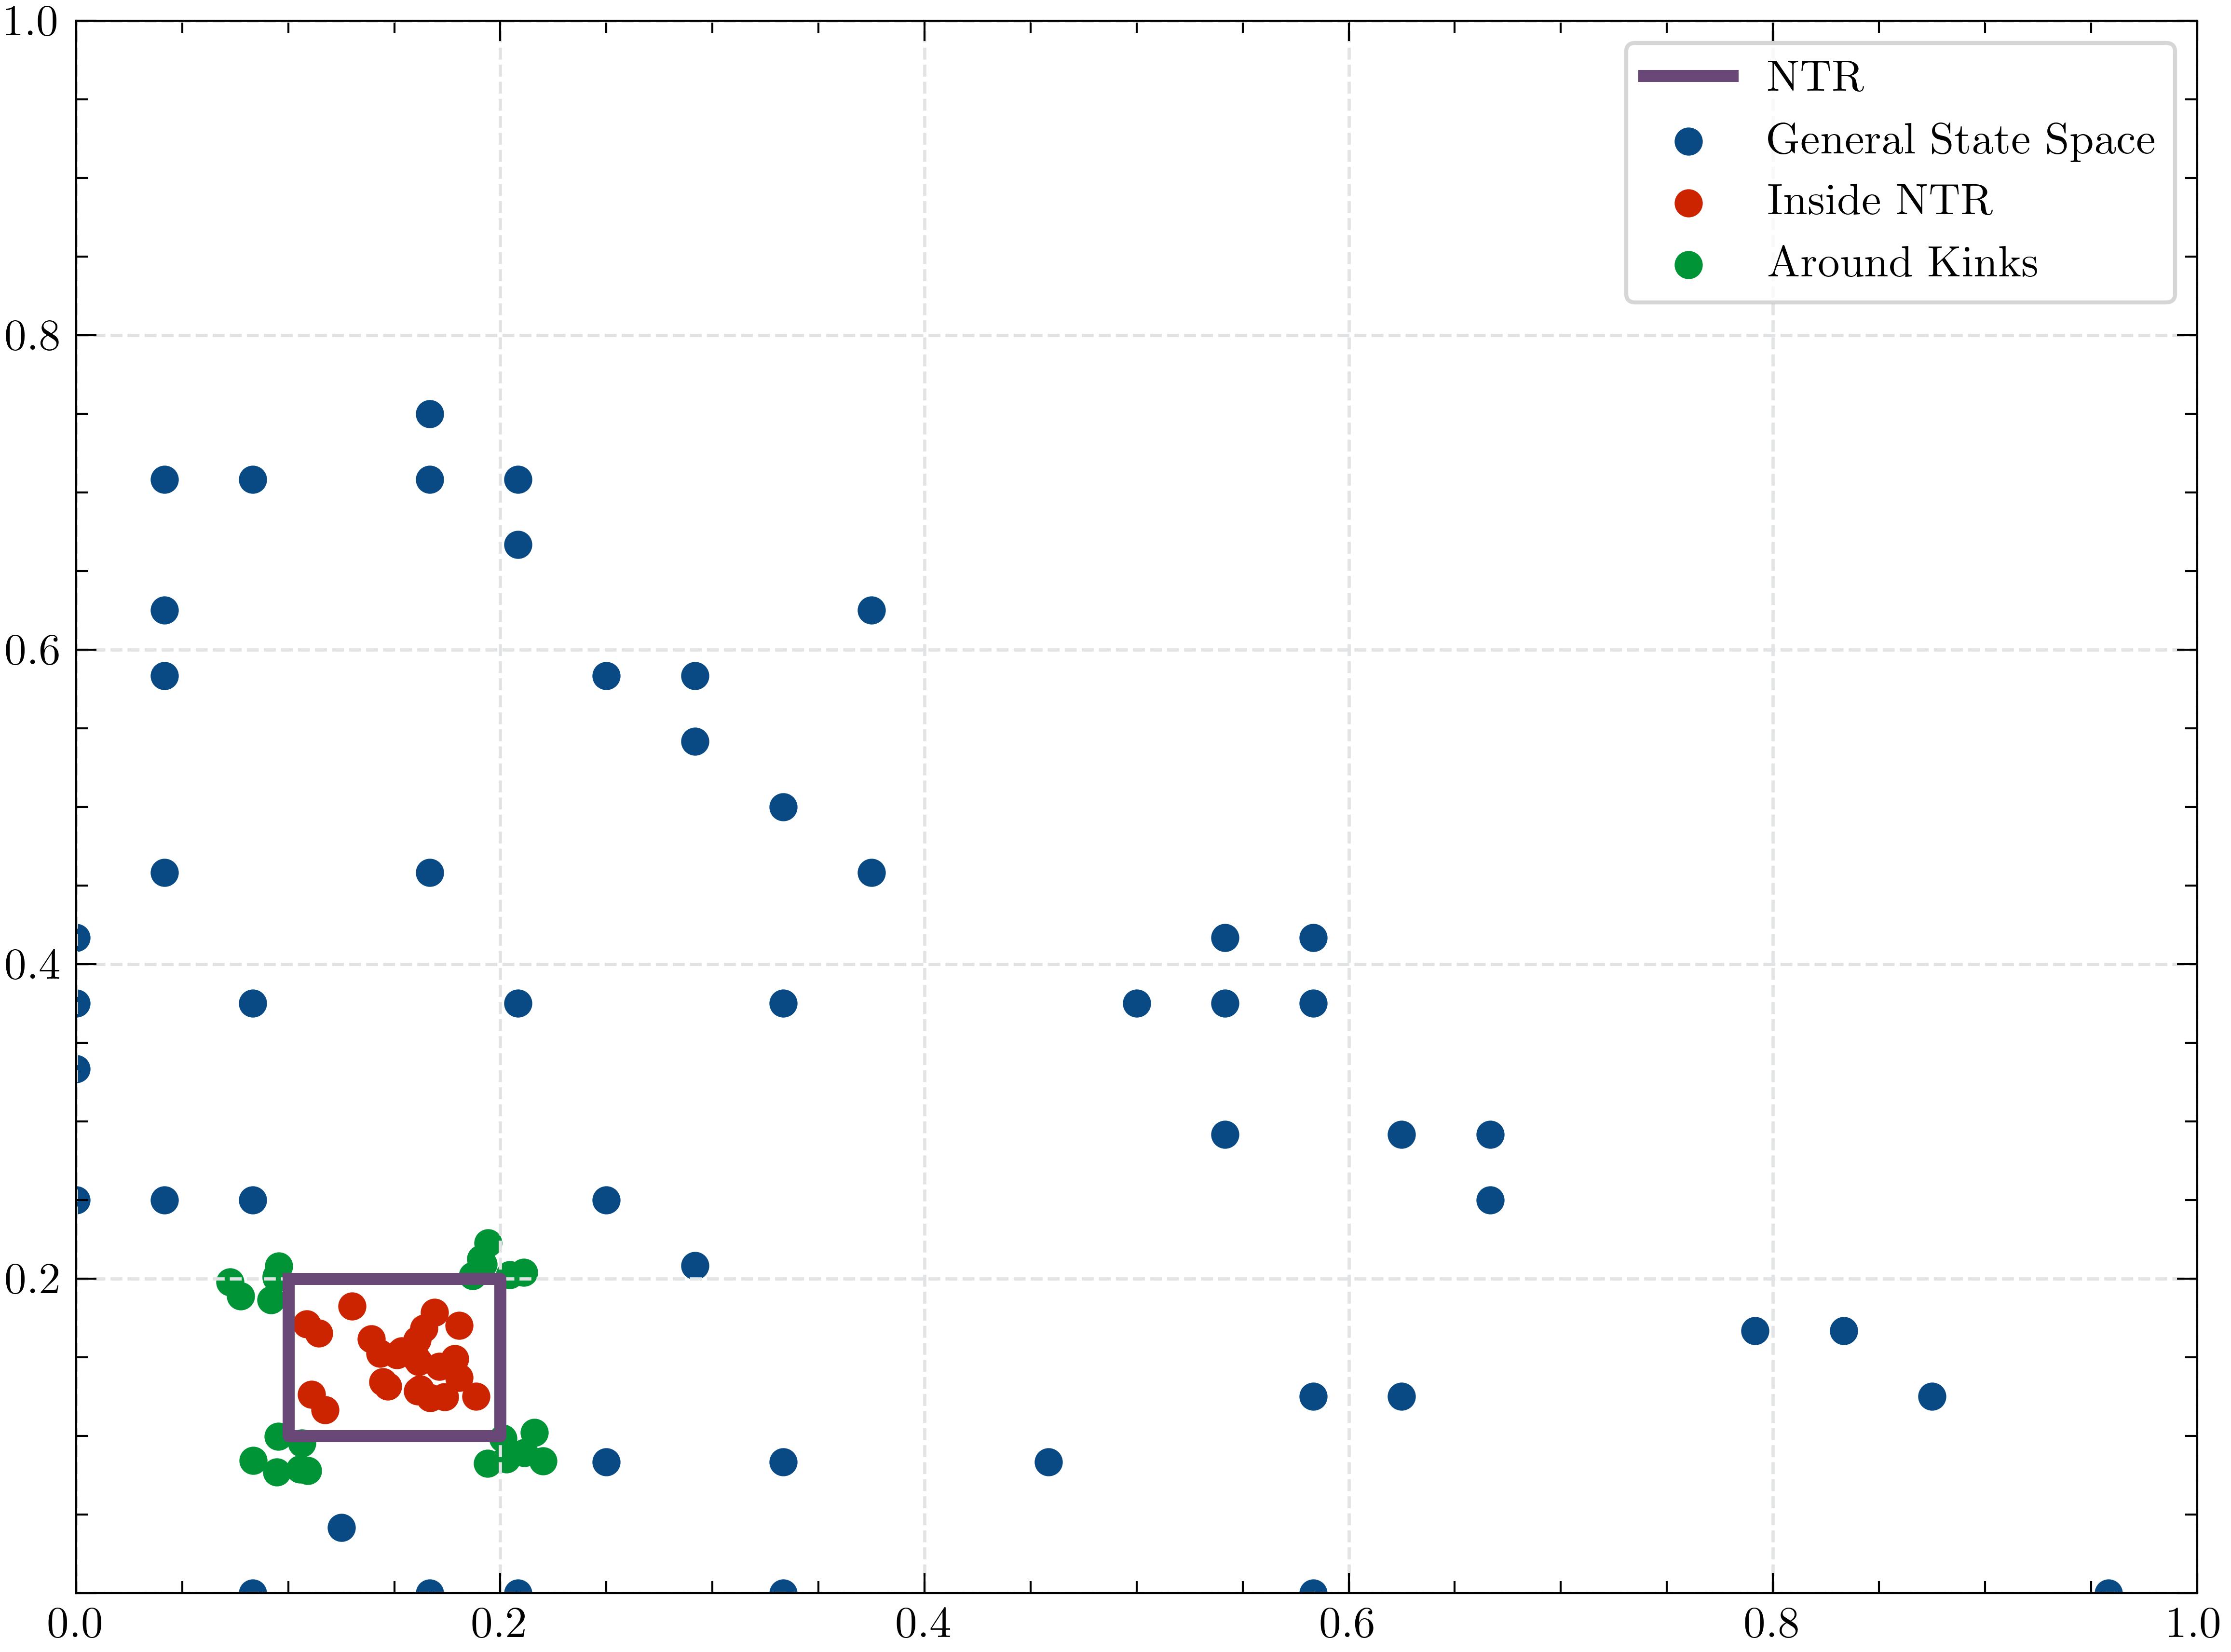
\includegraphics[scale = 0.3]{designed_sampling_strategy.png}
        \caption{The sampling strategy for the 2-dimensional case}
        \label{fig: Designed_sampling_strategy}
    \end{subfigure}%
    \hfill
    \begin{subfigure}[t]{0.48\textwidth}
        \centering
        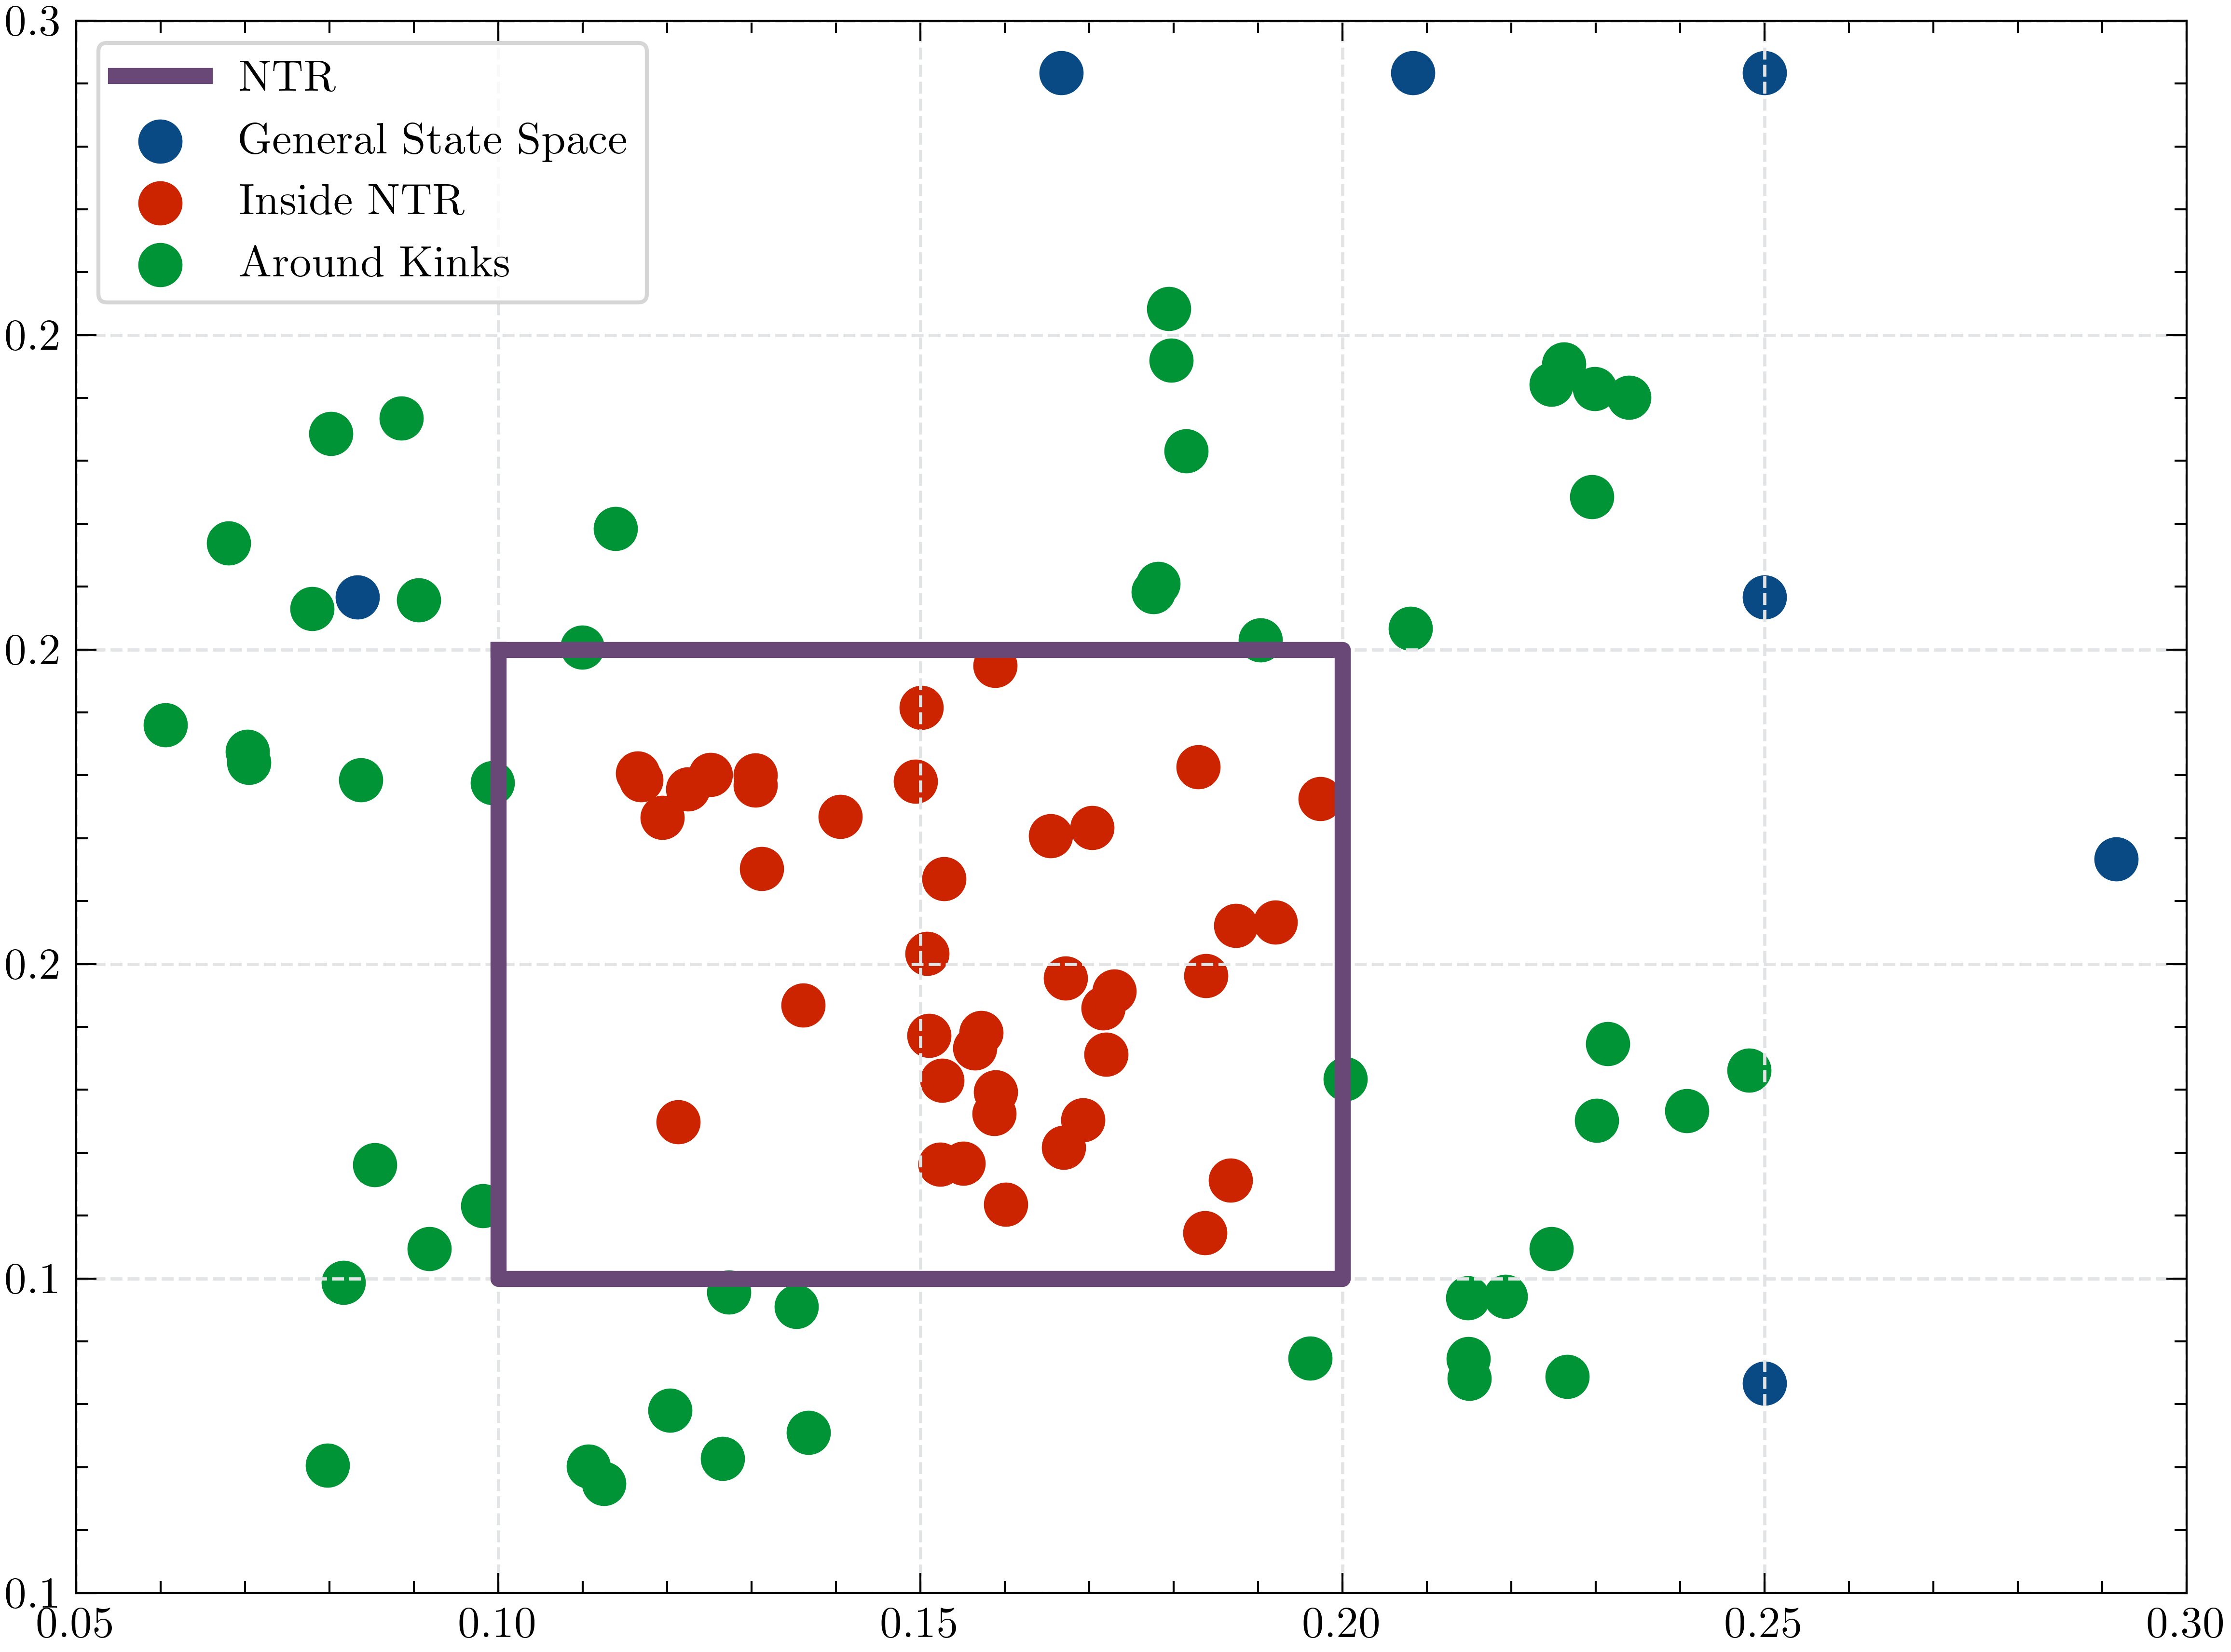
\includegraphics[scale = 0.3]{zoomed_designed_sampling_strategy.png}
        \caption{A zoom in on the \ac{NTR} for the sampling strategy}
        \label{fig: Designed_sampling_strategy-zoom}
    \end{subfigure}

% Overall caption
\caption{The designed sampling strategy for state space coverage.}
\floatfoot{\textbf{Note:} Sample consists of $N=200$ points, with $122$ points in the general state space ($55$\%), $40$ points inside the NTR ($20$\%) and $48$ points around the NTR kinks ($25$\%).}
\end{figure}

\subsubsection{Utilising the NTR approximation for $\boldsymbol{\delta}$ bounds} \label{Subsubsection: NTR-deltabounds}
Having constructed an efficient sampling strategy, i can further leverage the \ac{NTR} approximation to find bounds on the optimal policy $\boldsymbol{\delta}$,
for the optimization step for each of these points. For this consider the schematic \ac{NTR} in figure \ref{fig:no_trade_region_schematic}.
At each point outside the NTR, the optimal policy is to trade towards the boundary of the NTR. This can either mean trading towards a vertice of the \ac{NTR} or one of the faces.
For the blue regions, trading towards a vertice is optimal, and this means that the optimal policy is to reallocate in both risky assets.

In this case, we can set bounds on the optimal policy $\boldsymbol{\delta}$, by considering the euclidian distance to the \ac{NTR}.
Hence if i know beforehand, that for asset $1$ we need to sell (lower-right blue region), then i can set bounds on $\delta_{1}^{+}$ to $0$ and effectively remove this from the optimization problem.
I can likewise do this the other way around for the asset $2$, which i need to buy more of, and set bounds on $\delta_{2}^{+}$ to $0$.

For the green regions in the figure, the optimal policy is to trade towards a face of the \ac{NTR}, and this means that the optimal policy is to reallocate in one risky asset and hold the other.
I can therefore set bounds on the optimal policy $\boldsymbol{\delta}_{i}$ to $0$ for the asset which is to be held, and only consider reallocation in the second asset.

This method of setting bounds on the optimal policy $\boldsymbol{\delta}$ is a way to reduce the computational burden of the optimization problem, and to ensure that the optimization problem is well defined.
Furthermore, by knowing that the optimal policy reduces the euclidian distance to the \ac{NTR}, i can effectively remove policies which would suggest buying and selling the $i$th asset. 
\subsubsection{Multiple Gaussian Process Regressions} \label{Subsubsection: NTR-GPR}
The final ingredient in the algorithm is the use of multiple \ac{GPR}s.
Since i now can effectively sample points, and have information on their placement relative to the \ac{NTR},
i can leverage this, and estimate two seperate value functions, one inside the \ac{NTR} and one outside the \ac{NTR}.
This strategy effectively deals with the kinks of the \ac{NTR}, as this otherwise would pose a problem for any smooth function approximations.
I construct one \ac{GP} for the points inside the \ac{NTR}, and one for the points outside the \ac{NTR}, and when i then evaluate the value function at a point $v_{t+1}(\mathbf{x}_{t+1})$,
i select the appropriate \ac{GP} to evaluate the value function.

This is done after having optimized over the $N$ points from the sampling strategy, i construct two datasets:
\begin{align}
  \mathbf{X}_{t,\text{inside}} &= \{ \mathbf{x}_{t,i} , \hat{v}_{t,i} \mid \mathbf{x}_{t,i} \in \hat{\boldsymbol{\Omega}}_{t} \}\\
  \mathbf{X}_{t,\text{outside}} &= \{ \mathbf{x}_{t,i} , \hat{v}_{t,i} \mid \mathbf{x}_{t,i} \notin \hat{\boldsymbol{\Omega}}_{t} \}
\end{align}
Then each \ac{GP} is fit over the dataset, which consists of asset allocations and the corresponding value function output.
In the next period, $t-1$ (since we iterate backwards), i can then evalute the next period value functtion $v_{t+1}(\mathbf{x_{t+1}})$,
by selecting the appropriate \ac{GP}, and using the predictive mean from \eqref{eq: GP-pred-mean}:
\begin{equation} \label{eq: valuefunctin_gp_mean}
  \tilde{\mu}(\mathbf{x}_{t+1}) = k(\mathbf{x}_{t+1}, \mathbf{X}_{t+1}) [k(\mathbf{X}_{t+1}, \mathbf{X}_{t+1}) + \sigma^{2}_{\varepsilon} \mathbf{I}]^{-1} \hat{\mathbf{v}}_{t+1},
\end{equation}
\subsection{Final solution algorithms} \label{Subsection: Algorithm}
Now that each component regarding the solution algorithm has been covered, i can now presents the solution algorithms for the dynamic portfolio allocation problem, in pseudo code.
Starting at the second to last period, which is the last period where the investment decision is not trivial, the algorithm is as follows:
Sample $2^{D}$ points to approximate the \ac{NTR}. Then Approximate the \ac{NTR} by solving the optimization problem for these points.

Sample $N$ points in a strategic manner, as described in \ref{Subsubsubsection: Sample}. For each $x_{i,t} \in X_{t}$ with $\{ X_t \}^{N}_{i=1}$, solve the optimization problem to find the optimal policy $\boldsymbol{\delta}_{i}$.

Construct the datasets $\mathbf{X}_{t,\text{inside}}$ and $\mathbf{X}_{t,\text{outside}}$ and fit two \ac{GPR}s to the datasets $\mathbf{X}_{t,\text{inside}}$ and $\mathbf{X}_{t,\text{outside}}$.
The code can be split into two parts, algorithim (A) and algorithm (B). Algorithm A covers approximatin the NTR and algorithm B covers the entire \ac{DP} scheme.
These are drawn from the framework which has been covered, above, created by \autocite{Scheidegger2023}.

\begin{tcolorbox}[algobox]
\scriptsize{
\RestyleAlgo{algoruled}
\begin{algorithm}[H]
  \caption{Approximate the $t$-th period NTR in the discrete-time finite-horizon portfolio choice model with proportional transaction costs.}
  \Input{$t+1$ period's value function approximation $V_{t+1}$.}
  \Result{Set of approximated NTR vertices: $\{\hat{\boldsymbol{\omega}}_{i,t}\}_{i=1}^N$; Approximated NTR: $\hat{\boldsymbol{\Omega}}_t$.}
  Sample the set of $N = 2^D$ points $\tilde{\mathbf{X}}_t = \{\tilde{\mathbf{x}}_{t,i}\}_{i=1}^N$ using section strategy from Section \ref{Subsection: Approximating_NTR}.\\
  \For{$\tilde{\mathbf{x}}_{i,t} \in \tilde{\mathbf{X}}_t$}{
      Obtain policy $\hat{\boldsymbol{\delta}}_{i,t}$ for $\tilde{\mathbf{x}}_{i,t}$ by solving the optimization problem using $V_{t+1}$ as the next period's value function. (Terminal value function in $t=T-1$) \\
      Compute the approximate NTR vertices $\hat{\boldsymbol{\omega}}_{i,t} = \tilde{\mathbf{x}}_{i,t} + \hat{\boldsymbol{\delta}}_{i,t}$. \\
  }
  Compute the NTR approximation: $\hat{\boldsymbol{\Omega}}_t = \{\lambda \hat{\boldsymbol{\omega}}_t \mid \lambda \in (0,1)^N, \, \sum_{i=1}^N \lambda_i = 1\}$.
\end{algorithm}
}
\end{tcolorbox}


\begin{tcolorbox}[algobox]
\scriptsize{
\RestyleAlgo{algoruled}
\begin{algorithm}[H]
  \caption{Complete Dynamic programming scheme with Gaussian process regressions and the NTR approximation.}
  \Input{Terminal value function $v_T$; time horizon $T$; sample size $N$.}
  \Result{Set of GP approximations of the value functions $\{v_{t-1}\}_{t=0}^{T-1}$; set of approximated NTRs $\{\hat{\boldsymbol{\Omega}}_t\}_{t=0}^{T-1}$, obtained policies $ \{ \{\boldsymbol{\delta}\}^{N+2^{d}}_{i=1} \}_{0}^{T-1}$.}
  
  \BlankLine
  Set $\mathcal{V}_T = v_T$. \\
  \For{$t \in [T, \dots, 1]$}{
      Approximate NTR $\hat{\boldsymbol{\Omega}}_{t-1}$ (Alg.~1) using $\mathcal{V}_T$ as the next period's value function. \\
      Sample $N$ points $\mathbf{X}_{t-1} = \{\mathbf{x}_{t-1,i}\}_{i=1}^N$ using the constructed sampling scheme. \\
      \For{$\mathbf{x}_{i,t-1} \in \mathbf{X}_{t-1}$}{
          Obtain value $\hat{v}_{i,t-1}$ and policy $\{\hat{\delta}_{i,t-1}, \hat{c}_{i,t-1}\}$ for $\mathbf{x}_{i,t-1}$ by solving the optimization problem using $\mathcal{V}_t$ as the next period’s value function. \\
      }
      Define the training sets:
      \begin{align*}
      \mathcal{D}_{\text{in},t-1} &= \{ (\mathbf{x}_{i,t-1}, \hat{v}_{i,t-1}) \mid \mathbf{x}_{i,t-1} \in \hat{\boldsymbol{\Omega}}_{t-1} \}, \\
      \mathcal{D}_{\text{out},t-1} &= \{ (\mathbf{x}_{i,t-1}, \hat{v}_{i,t-1}) \mid \mathbf{x}_{i,t-1} \notin \hat{\boldsymbol{\Omega}}_{t-1} \}.
      \end{align*}
      Given $\mathcal{D}_{\text{in},t-1}$ and $\mathcal{D}_{\text{out},t-1}$, approximate $v_{t-1}$ for inside and outside of the NTR $\{G_{\text{in},t-1}, G_{\text{out},t-1}\}$ (using the respective datasets) with GPs. \\
      Set $v_{t-1} = \{G_{\text{in},t-1}, G_{\text{out},t-1}\}$.
  }
  \end{algorithm}
}
\end{tcolorbox}

\subsection{Computational stack and implementation} \label{Subsection: Computational_stack}
The solution algorithm is implemented in Python, and takes advantage of a simple but powerfull computational stack. following \autocite{Scheidegger2023}.
The economic identities and dynamic where written using the \texttt{PyTorch} package, which is a machine learning library implemented in Python.
This package has an auto-differentiation feature, which allows for easily implmentable gradients for the constrainted optimization scheme.
Furthermore this package is also directly linked with the \texttt{GPyTorch} package, which is a Gaussian process library implemented using PyTorch.
The \ac{GPR}s were implemented using the \texttt{GPyTorch} package, which is a Gaussian process library implemented using PyTorch.
This package has multiple speedups for \ac{GPR}s, such as the LancZos Variance Estimate (LOVE) and the SKIP method, which reduces the computational burden of the \ac{GPR}s.
Furthermore the predictive mean can be computed using black-box matrix-matrix multiplication, which is a speedup for the predictive mean computation,
skipping cholesky decompositions for large matrices.\\
The constrained optimizer i use is the \texttt{Cyipopt} package, which is a Python wrapper for the \texttt{Ipopt} package, which is a non-linear optimization package.
This package is used to solve the optimization problem for each point in the state space, and is used to find the optimal policy $\boldsymbol{\delta}$ for each point.\\
The gaussian quadrature grid-points where implemented with the \texttt{Tasmanian} package, which is a sparse grid package.
This was taken from \autocite{Schober2022}, who used this package to implement sparse adaptive grids.\\
Finally i implemented parallelization at two points in the code. Whenever we run the optimization scheme for a point in the state space, we can run these in parallel,
as they are independent operations, as long as i do this within the same timepoint $t$.

\subsubsection{Optimization details} \label{Subsubsection: optimization_details}
When solving the optimization problem, i use a tolerance of $10^{-7}$, and $1000$ iterations.
When approximating the \ac{NTR}, i solve for each point $8$ times, and select the optimal solution among these.
Furthermore i multiply the starting point with a decaying factor, in the number of starts,
in order to add small variance at each iteration. This is because non-linear optimization problems can be
sensitive to the initial starting points.

The initial starting point is chosen within the feasible space at random, when there is no approximated \ac{NTR}.
The random draws are chosen to be feasible given the constraints of the problem.
When i later have approximated the \ac{NTR}, i use the shortest distance towards the \ac{NTR} as initial guess,
and multiply with a decaying factor over the number of starts. For these points i solve the optimization problem $3$ times.
This is because when i can leverage the knowledge of the \ac{NTR}, the optimization problem is easier.

For points inside the \ac{NTR} i likewise guess no trading, knowing this to be optimal a-priori.
Small jitter is added to this when using multiple solutions.



\ifdefined\COMPILINGMAIN
% Main file is compiling this section, skip the end
\else
% \printbibliography
\end{document}
\fi

\newpage

\begingroup 
  \hypersetup{linkcolor=black}

  \hypersetup{
    colorlinks=true,
    citecolor=black,
    linkcolor=black,
    filecolor=black, 
    urlcolor=black}
  \printbibliography
\endgroup

\newpage

\ifdefined\COMPILINGMAIN
% Main file is compiling this section, skip the preamble
\else
% Individual file compilation
\documentclass[11pt]{article}
% Geometry and page layout
\usepackage{geometry}
\geometry{verbose,tmargin=3.375cm,bmargin=2cm,lmargin=3.375cm,rmargin=3.375cm}

% Input encoding and font settings
\usepackage[utf8]{inputenc}

% other fonts
%Slightly more bold
% \usepackage{mlmodern}
% \usepackage[T1]{fontenc}

%Moder modern look
% \usepackage{libertine}
% \usepackage{libertinust1math}
% \usepackage[T1]{fontenc}

\usepackage{amsfonts, amsmath, amsthm, bbm, setspace}
\onehalfspacing
\usepackage{algorithm2e}
\usepackage{tcolorbox} % For the grey background
% Create a tcolorbox style for the algorithm
\tcbuselibrary{listingsutf8}
\tcbset{
    algobox/.style={
        colback=gray!3, % Background color
        colframe=black,  % Border color
        sharp corners,   % Square corners
        boxrule=0.5pt,   % Border thickness
        before skip=10pt, % Vertical spacing before box
        after skip=10pt,  % Vertical spacing after box
        width=\textwidth, % Box width
    }
}

% Adjust algorithm2e settings for a similar look
\SetKwInOut{Input}{Input}
\SetKwInOut{Result}{Result}
\SetKwFor{For}{for}{:}{end}

% Adjust settings for algorithm2e
\SetAlgoCaptionSeparator{.} % Separator for caption
\SetAlgoNlRelativeSize{-2}  % Adjust line number font size
\SetAlgoInsideSkip{2pt}    % Reduce space between lines
\SetAlCapSkip{0pt}         % Remove extra space after the caption
% Ensure captions are above algorithms
\SetAlgoCaptionLayout{center} % Center caption
% Adjust the style of the algorithm to remove bottom line
\RestyleAlgo{ruled}
\SetAlCapSkip{0.5em}       % Space after caption
\SetAlgoVlined              % Ensures no horizontal lines at the end

% Theorem and math environments
\newtheorem{assumption}{Assumption}
\newtheorem{lemma}{Lemma}
\newtheorem{theorem}{Theorem}

% New math commands
\newcommand{\npsym}{\mathrel{\ooalign{\raisebox{.6ex}{$>$}\cr\raisebox{-.6ex}{$<$}}}}

% Table formatting
\usepackage{booktabs, multirow, array, tabularx}
\newcolumntype{N}{>{\centering\arraybackslash}m{.85in}}

% Caption settings
\usepackage{caption}
\captionsetup{format=plain, font=footnotesize, labelfont=bf,width=3.5in}
\setlength{\abovecaptionskip}{3pt plus 3pt minus 3pt}

% Figures and floats setup
\usepackage{graphicx, adjustbox,subcaption}
\usepackage{floatrow}
\floatsetup[figure]{capposition=top}
\floatsetup[table]{capposition=top}
\renewcommand\thefigure{\thesection.\arabic{figure}}
% Path to figures
\graphicspath{{../Figures/}}
\usepackage{tikz} % TikZ for creating figures
% URLs and references and colors
\usepackage[dvipsnames]{xcolor}
\usepackage[hyphens]{url}
\usepackage{hyperref}
\hypersetup{
    colorlinks=true,
    citecolor=[HTML]{901A1E}, %KU red
    linkcolor=[HTML]{901A1E}, %KU red    
    filecolor=blue, 
    urlcolor=[HTML]{901A1E}, %KU red
    hyperindex=true,
    hyperfigures=true,
    hyperfootnotes=true,
}

% Biblatex settings for references
\usepackage[style=authoryear, dashed=false, backend=bibtex]{biblatex}
\addbibresource{../Ref.bib}

\renewbibmacro*{volume+number+eid}{%
  \printfield{volume}%
  \setunit*{\addcomma\space}%
  \printfield{number}%
  \setunit{\addcomma\space}%
  \printfield{eid}
}
\DeclareFieldFormat[article]{volume}{\bibstring{volume}~#1}
\DeclareFieldFormat[article]{number}{\bibstring{number}~#1}
\DefineBibliographyStrings{english}{volume = {Vol.}, number = {No.}}

% Author name formatting
\DeclareNameAlias{author}{last-first}
\renewcommand*{\finalnamedelim}{\addspace and\space}
\renewcommand*{\multinamedelim}{\addcomma\space}

% Footnotes and appendix setup
\usepackage[hang,flushmargin]{footmisc}
\usepackage[toc,page]{appendix}
\renewcommand\appendixtocname{Appendices}
\renewcommand\appendixpagename{Appendices}

%# Assumptions like theorems and corrolaries
% {
%   \theoremstyle{plain}
%   \newtheorem{assumption}{Assumption}
% }
% Title setup
\usepackage{titlepic}
\usepackage{titlesec}
\titleformat{\section}{\normalfont\Large\bfseries}{\thesection}{1em}{}[{\titlerule[0.1pt]}]
% no text above figures!!!!
\usepackage{placeins}

% Abbreviations (acronym package)
\usepackage{acro}
\acsetup{list/name = Abbreviations}
\DeclareAcronym{PML}{short=PML, long= Probabilistic Machine Learning}
\DeclareAcronym{NTR}{short=NTR, long=No-Trade Region}
\DeclareAcronym{MC}{short=MC, long=Monte Carlo}
\DeclareAcronym{QMC}{short=QMC, long=Quasi-Monte Carlo}
\DeclareAcronym{RQMC}{short=RQMC, long=Randomized Quasi-Monte Carlo}
\DeclareAcronym{LDS}{short = LDS, long = Low-Discrepancy Sequences}
\DeclareAcronym{LLN}{short = LLN, long = Law of Large Numbers}
\DeclareAcronym{GPR}{short = GPR, long = Gaussian process regression}
\DeclareAcronym{GP}{short = GP, long = Gaussian process}
\DeclareAcronym{ARD}{short = ARD, long = Automatic Relevance Detection}
\DeclareAcronym{LOVE}{short = LOVE, long = LanczOS Variance Estimates}
\DeclareAcronym{SKIP}{short = SKIP, long = Structured Kernel Interpolation for Products}
\DeclareAcronym{SGD}{short = SGD, long = Stochastic Gradient Descent}
\DeclareAcronym{DP}{short = DP, long = Dynamic Programming}
\DeclareAcronym{MPT}{short=MPT, long=Modern Portfolio Theory}


% Conditional macro for compiling individual files
\ifdefined\COMPILINGMAIN
% Define settings when compiling the main document
\else
% Define minimal preamble for individual file compilation
\usepackage{geometry}
\geometry{verbose,tmargin=3.375cm,bmargin=2cm,lmargin=3.375cm,rmargin=3.375cm}
\fi

\AtBeginDocument{%
    \renewcommand{\contentsname}{Table of Contents}
    \renewcommand{\abstractname}{Abstract}
}
\setlength\parindent{11pt}
% Define the macro for compiling the main file
%\def\COMPILINGMAIN{}  % Include the main preamble
\begin{document}
\fi

\begin{appendices}
\numberwithin{equation}{section}
\numberwithin{figure}{section}
\addtocontents{toc}{\protect\setcounter{tocdepth}{0}}


\section{Other sampling strategies}\label{section: Appendix-sample}
\begin{figure}[h!]
  \begin{center}
  \caption{Uniform grid sampling strategy} 
  \label{fig: uniform_grid}
  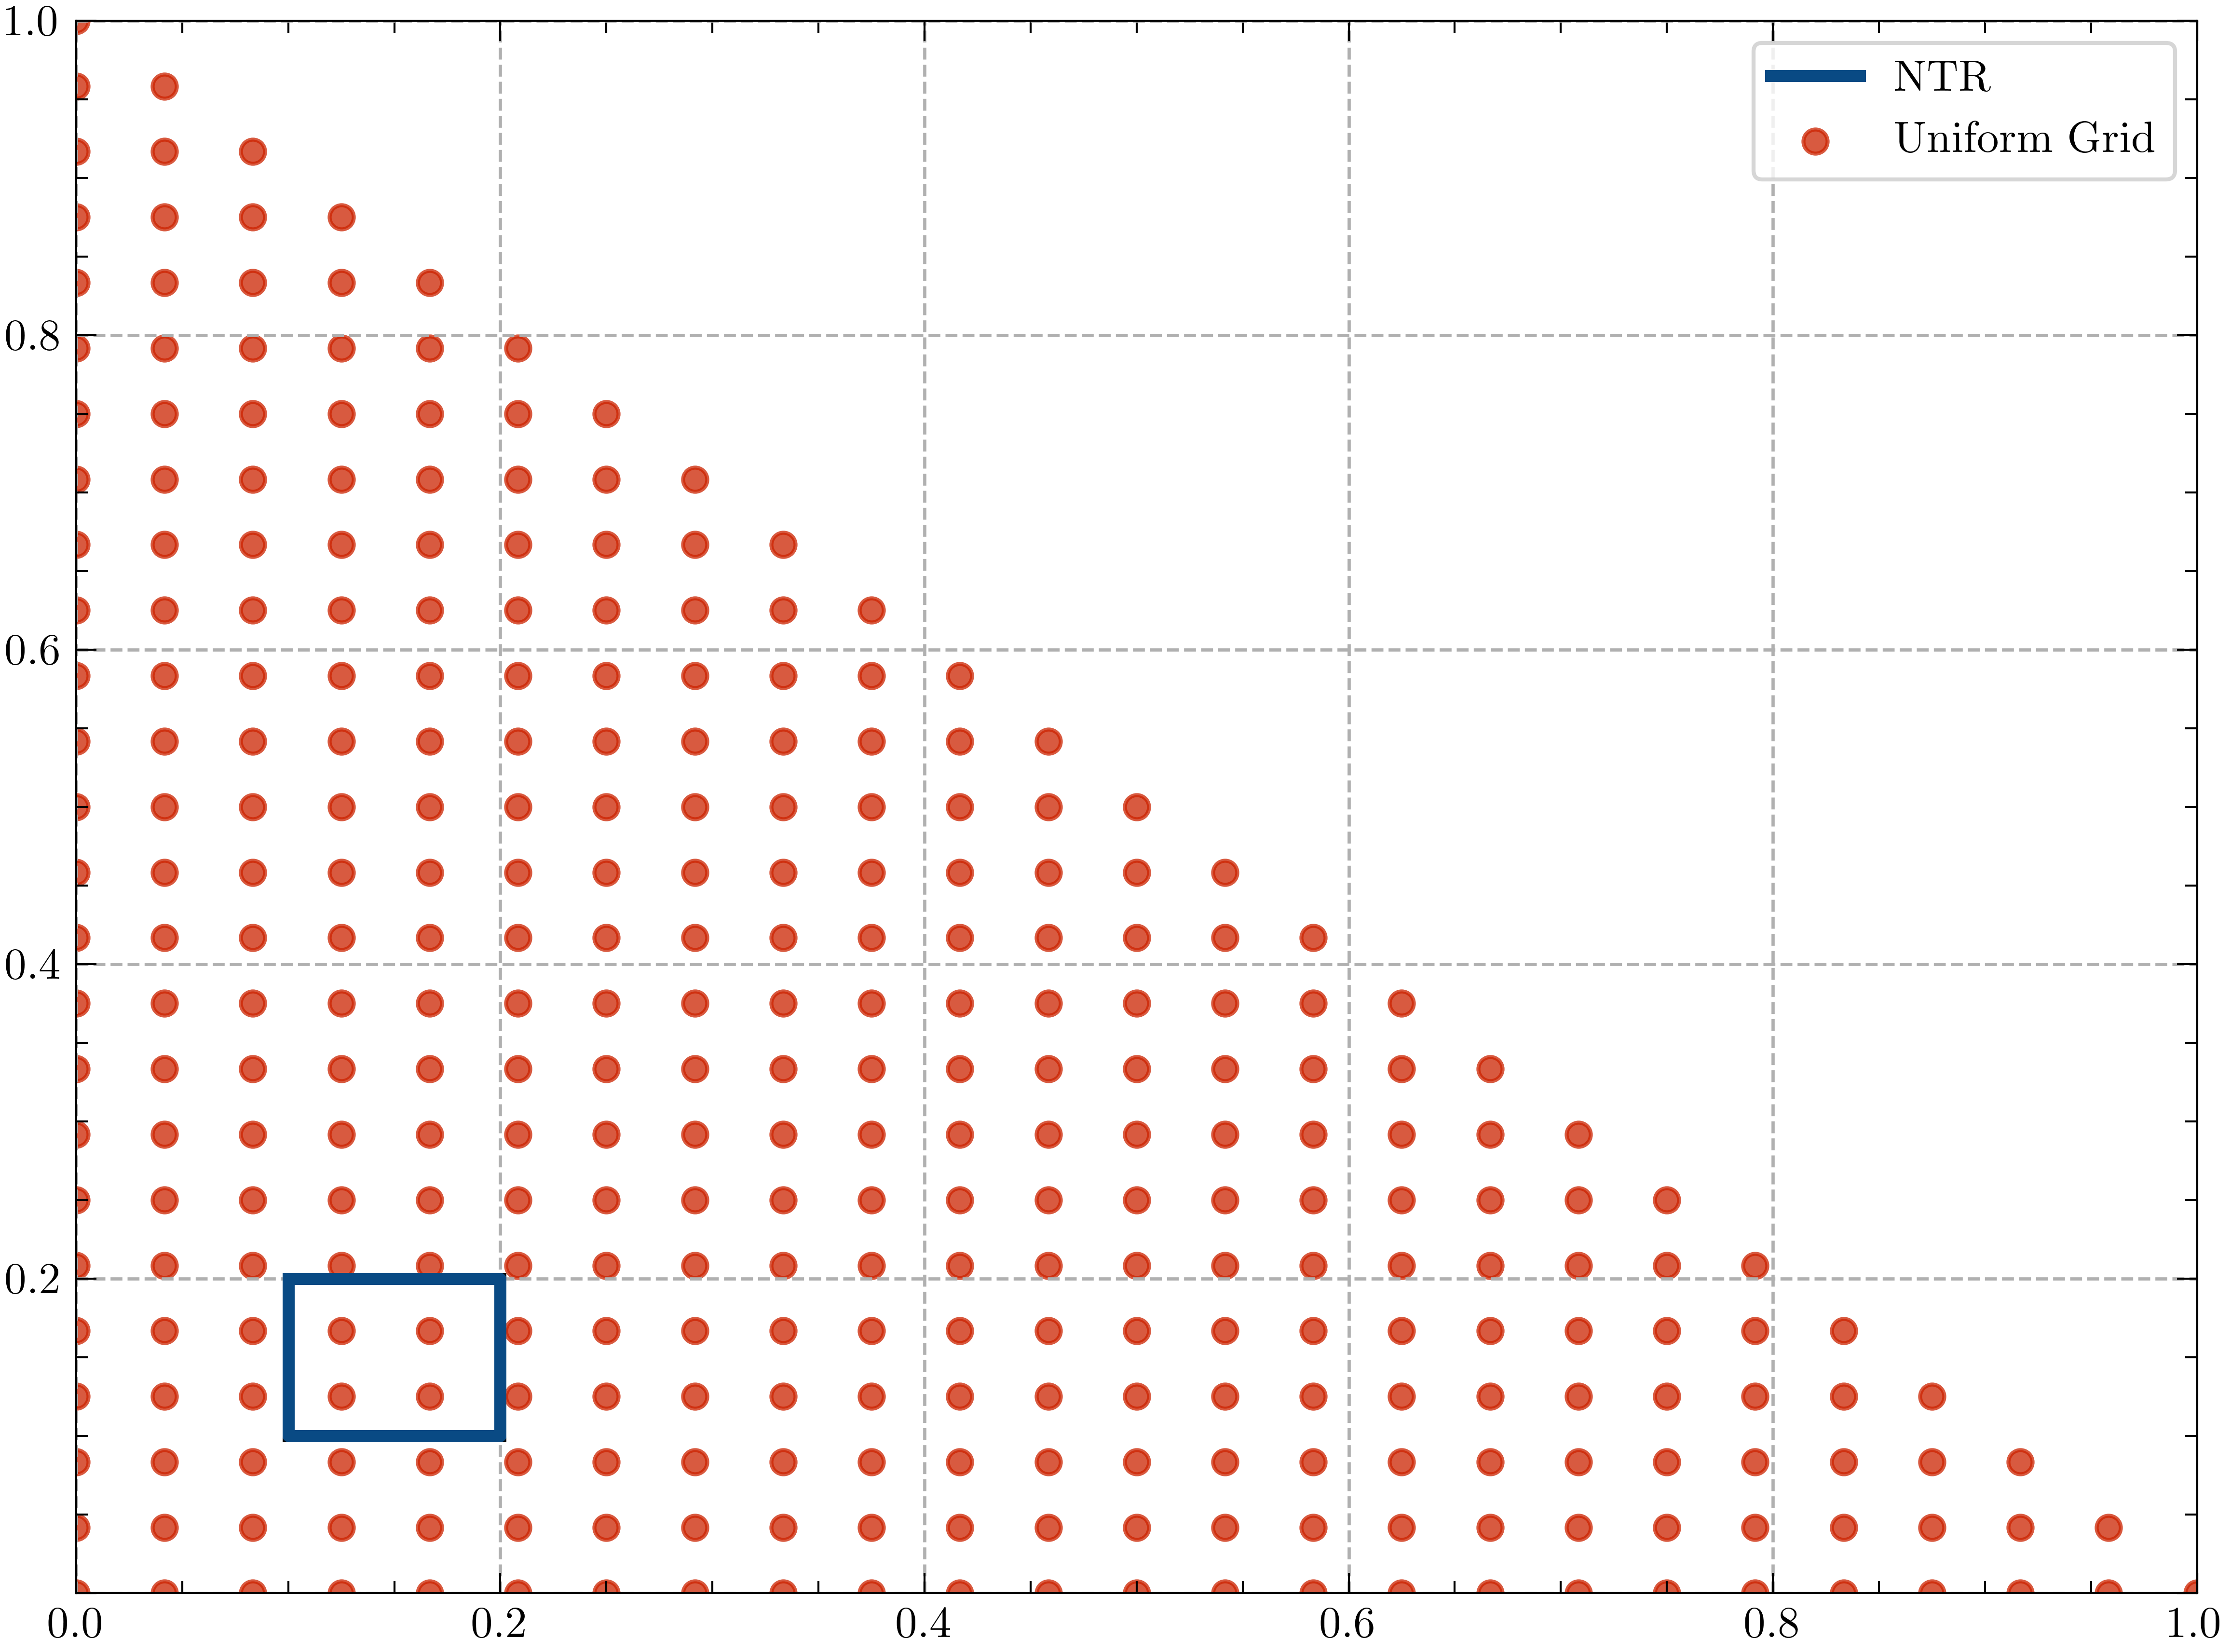
\includegraphics[scale=0.34]{uniform_grid.png}
  \end{center}
  \floatfoot{\textbf{Note:} Sample consists of $N=200$ points.}
  \end{figure}

  \begin{figure}[h!]
    \begin{center}
    \caption{Naive random sampling strategy} 
    \label{fig: random_sample}
    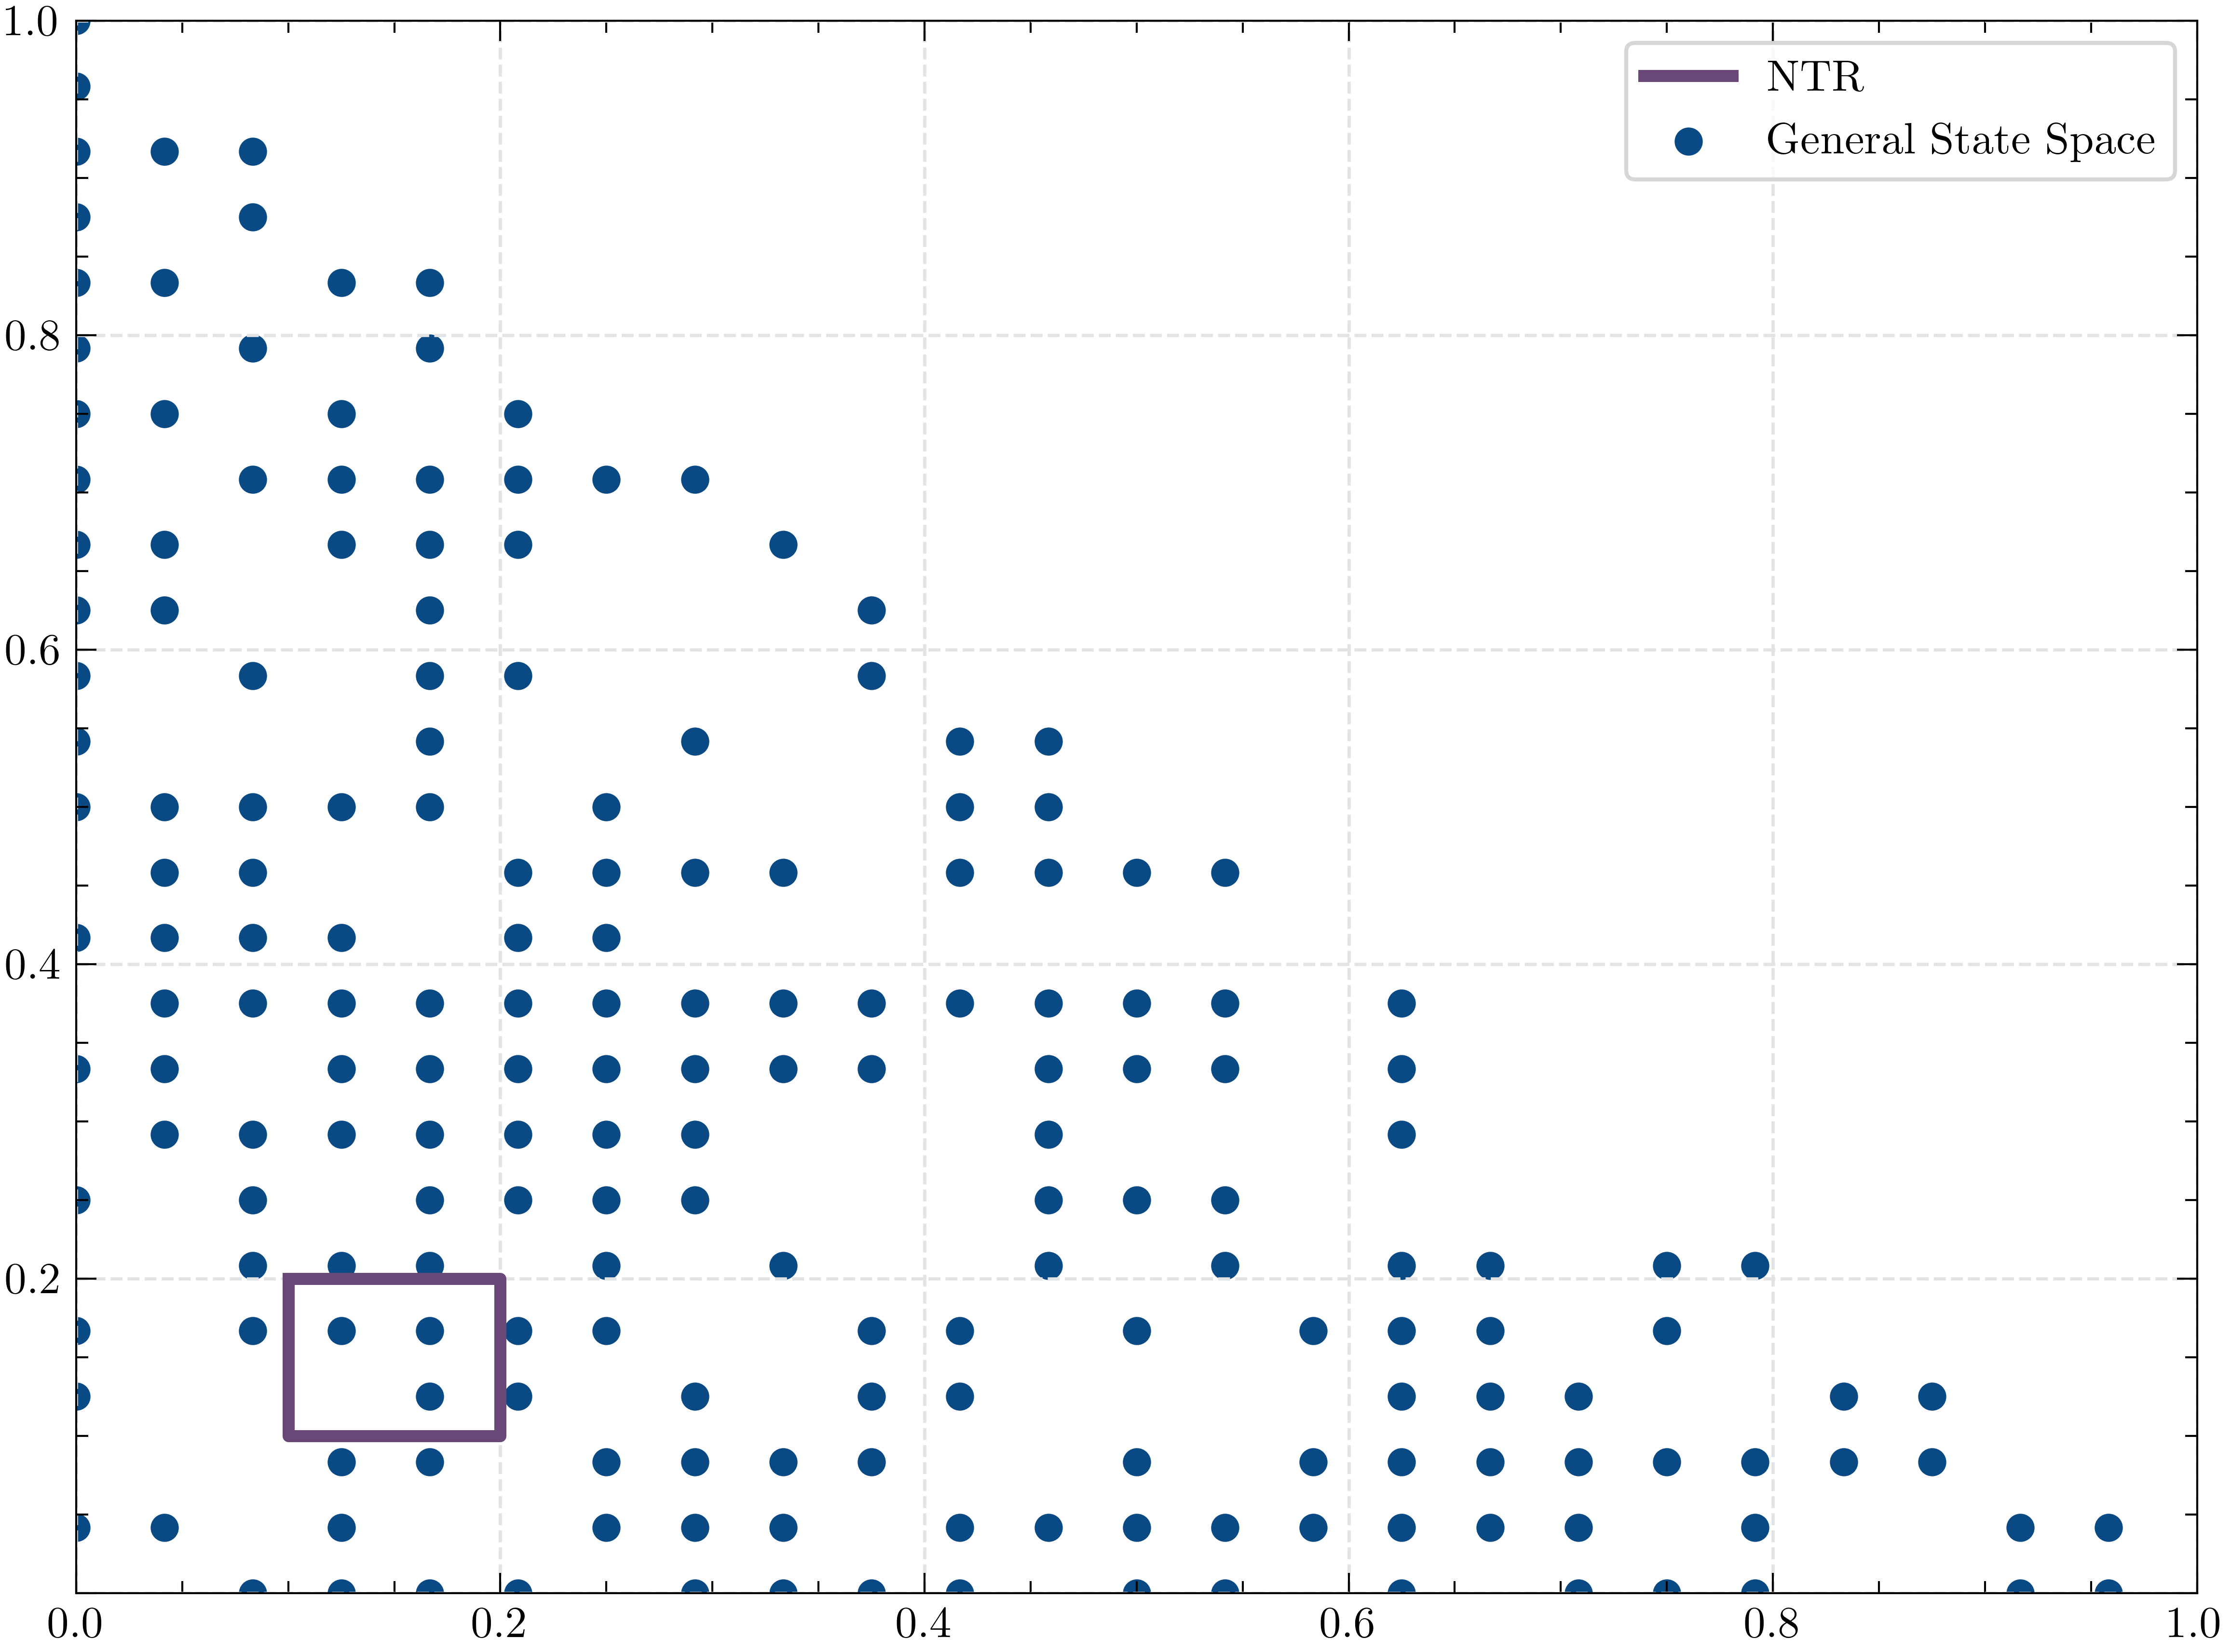
\includegraphics[scale=0.34]{naive_sampling_strategy.png}
    \end{center}
    \floatfoot{\textbf{Note:} Sample consists of $N=200$ points.}
    \end{figure}

\section{Extended asset space parameters}\label{section: Extended asset universe}

\[
\mu = 
\begin{bmatrix}
0.0572 \\
0.0638 \\
0.07 \\
0.0764 \\
0.0828 \\
0.06 \\
0.07 \\
\end{bmatrix}
\]

\[
\Sigma = 
\begin{bmatrix}
0.0256 & 0.00576 & 0.00288 & 0.00176 & 0.00096 & 0.002 & -0.001 \\
0.00576 & 0.0324 & 0.00904 & 0.01069 & 0.01296 & 0 & -0.002 \\
0.00288 & 0.00904 & 0.04 & 0.0132 & 0.0168 & 0 & -0.0015 \\
0.00176 & 0.01069 & 0.0132 & 0.0484 & 0.02112 & 0 & -0.001 \\
0.00096 & 0.01296 & 0.0168 & 0.02112 & 0.0576 & 0 & -0.0005 \\
0.002 & 0 & 0 & 0 & 0 & 0.02 & 0 \\
-0.001 & -0.002 & -0.0015 & -0.001 & -0.0005 & 0 & 0.025 \\
\end{bmatrix}
\]

\[
% \text{}
\operatorname{Corr} =
\begin{bmatrix}
1 & 0.2 & 0.09 & 0.05 & 0.025 & 0.0884 & -0.0395 \\
0.2 & 1 & 0.2512 & 0.27 & 0.3 & 0 & -0.0703 \\
0.09 & 0.2512 & 1 & 0.3 & 0.35 & 0 & -0.0474 \\
0.05 & 0.27 & 0.3 & 1 & 0.4 & 0 & -0.0287 \\
0.025 & 0.3 & 0.35 & 0.4 & 1 & 0 & -0.0132 \\
0.0884 & 0 & 0 & 0 & 0 & 1 & 0 \\
-0.0395 & -0.0703 & -0.0474 & -0.0287 & -0.0132 & 0 & 1 \\
\end{bmatrix}
\]

\section{Fitting the $3$D fixed cost NTRs}\label{section: Fitting_Ellipse_Appendix}
\begin{figure}[!ht]
  \centering
  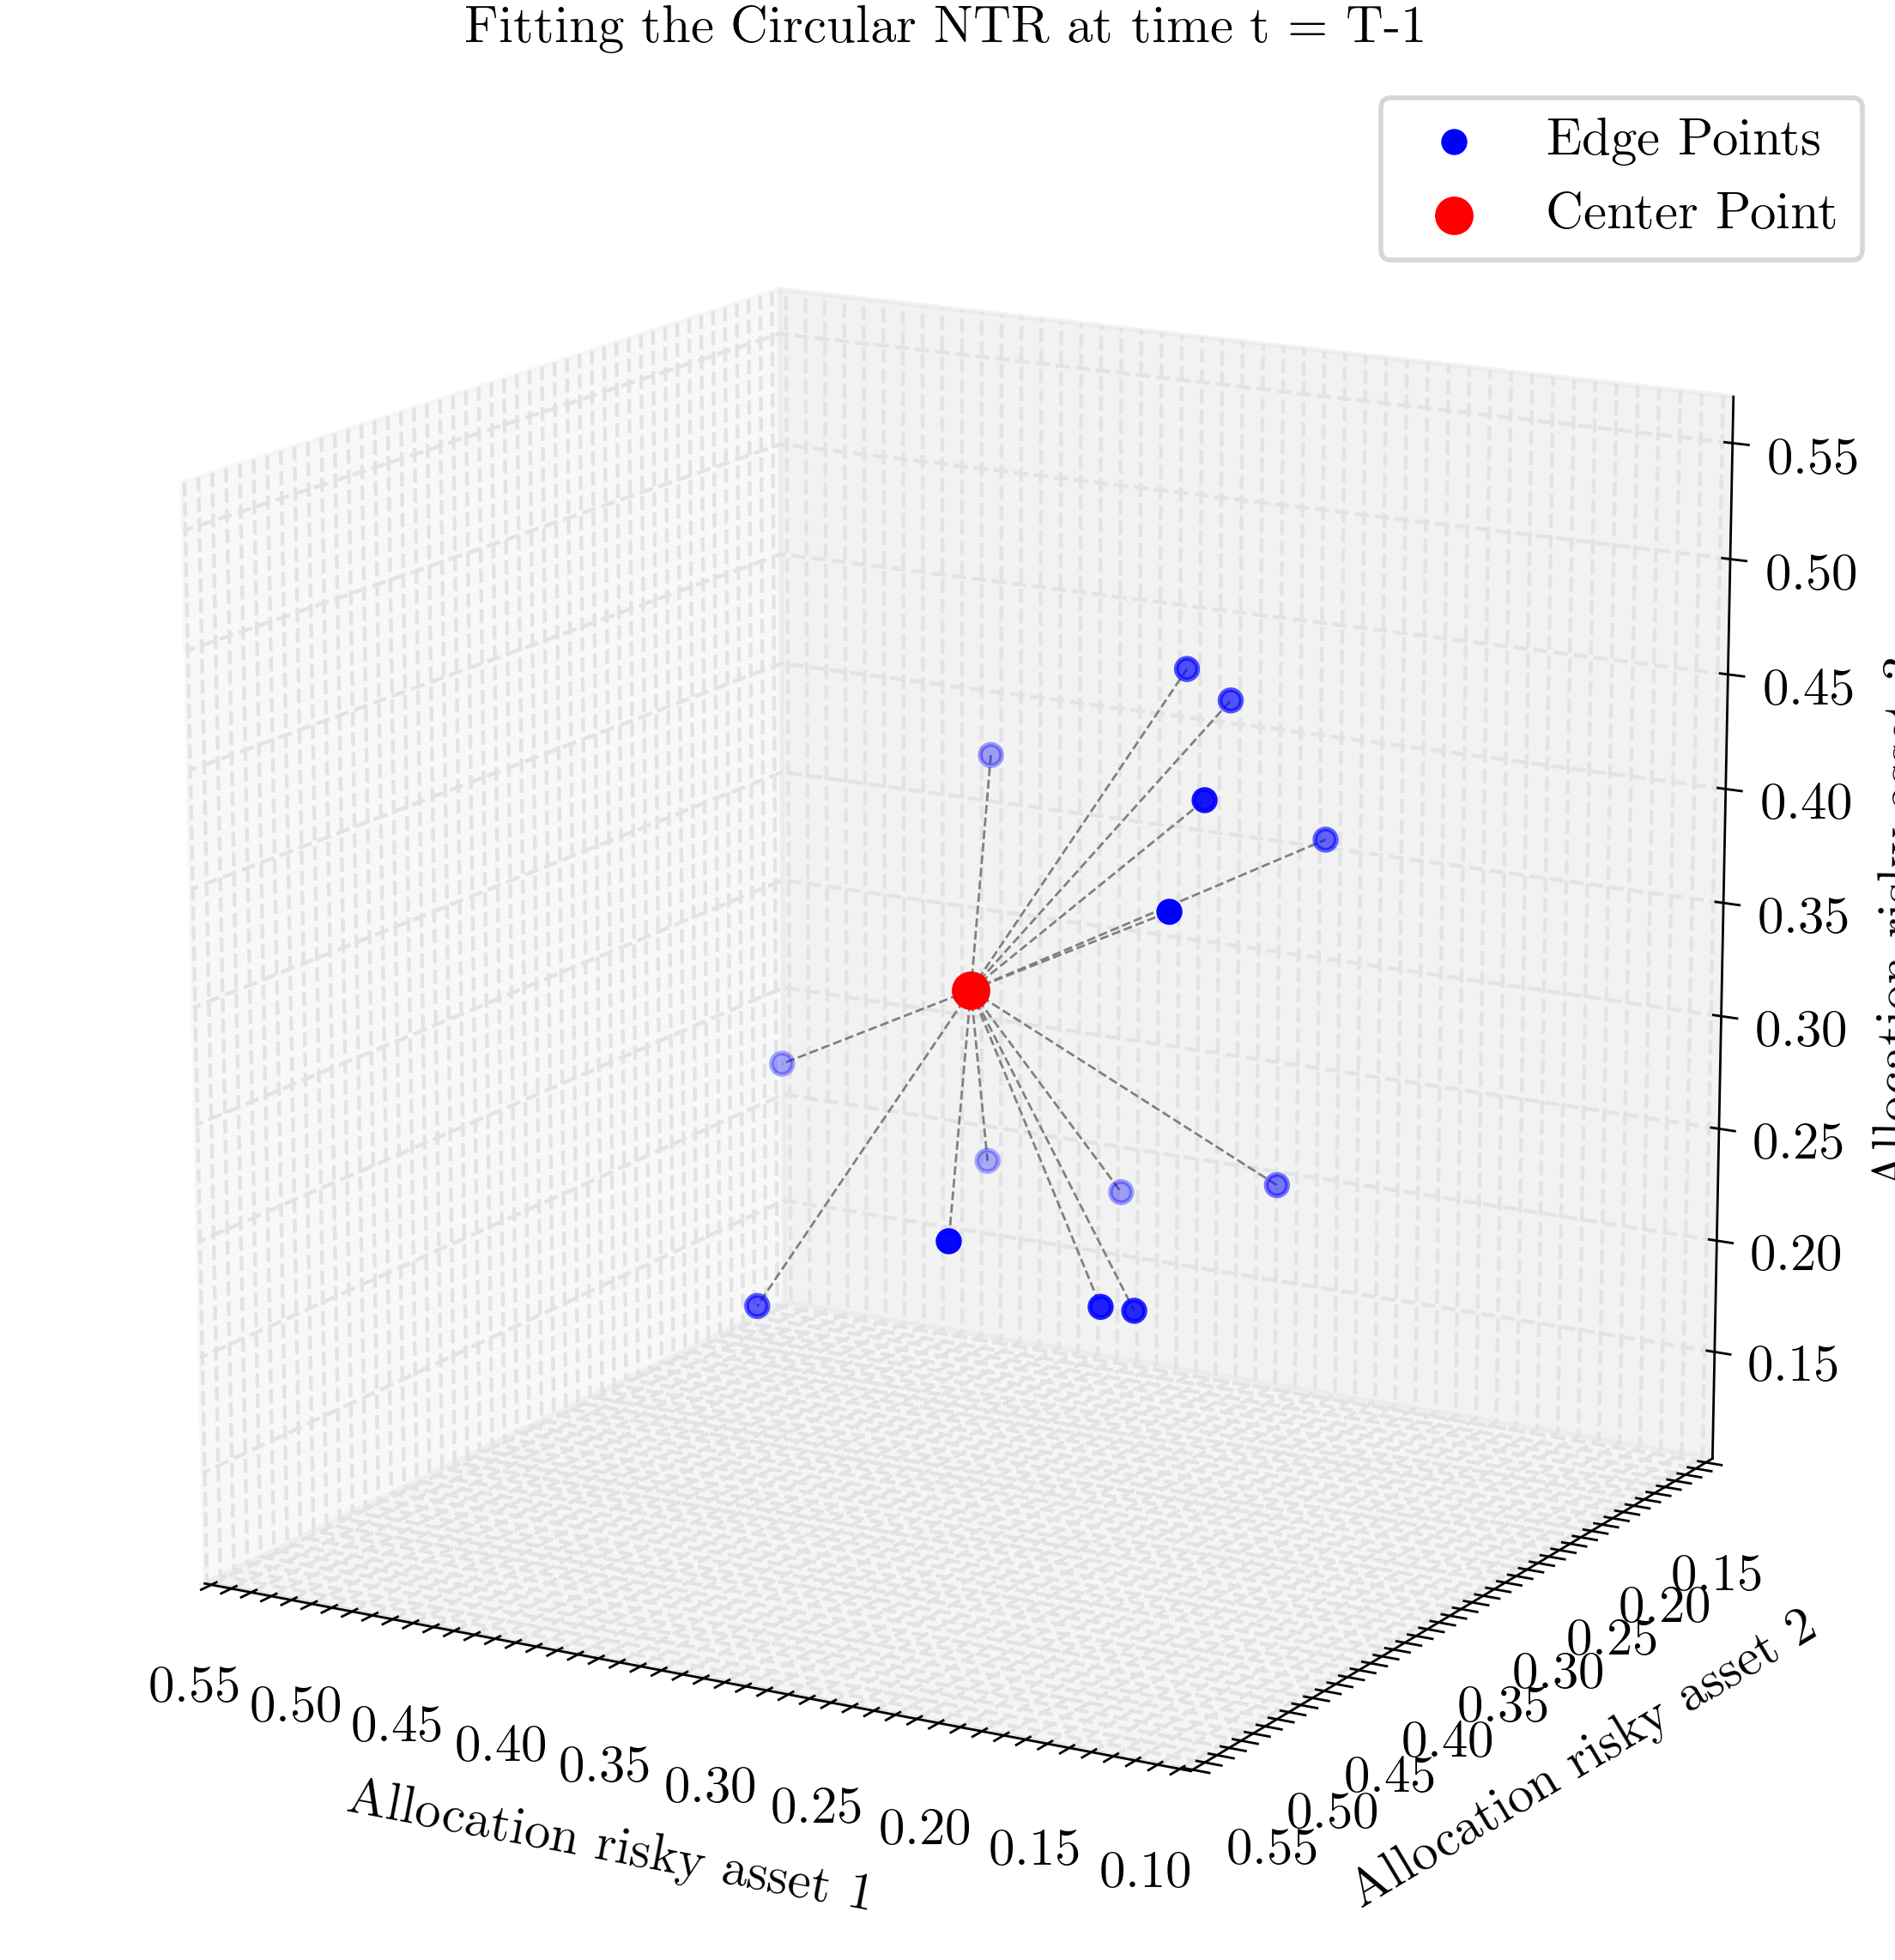
\includegraphics[scale = 0.38]{Fitting_Circular_NTR_iid_3_d.png}
  \caption{Fitting shceme for the $3$D sphere NTR}
  \label{fig: Sphere_Fitting_Appendix}
  \floatfoot{Fitting the sphere NTR with $3$D data uses $14$ points, more than necessary, to ensure a good fit}
\end{figure}

\end{appendices}
\ifdefined\COMPILINGMAIN
% Main file is compiling this section, skip the end
\else
% \printbibliography
\end{document}
\fi

\end{document}
